%%%%%%%%%%%%%%%%%%%%%%%%%%%%%%%%%%%%%%%%%%%%%%%%%%%
%% LaTeX book template                           %%
%% Author:  Amber Jain (http://amberj.devio.us/) %%
%% License: ISC license                          %%
%%%%%%%%%%%%%%%%%%%%%%%%%%%%%%%%%%%%%%%%%%%%%%%%%%%
\documentclass[12pt,french,twoside,openright]{book}

%\documentclass[a4paper,11pt]{book}
\usepackage[T1]{fontenc}
\usepackage[utf8]{inputenc}
\usepackage{lmodern}
%%%%%%%%%%%%%%%%%%%%%%%%%%%%%%%%%%%%%%%%%%%%%%%%%%%%%%%%%
% Source: http://en.wikibooks.org/wiki/LaTeX/Hyperlinks %
%%%%%%%%%%%%%%%%%%%%%%%%%%%%%%%%%%%%%%%%%%%%%%%%%%%%%%%%%
\usepackage{hyperref}
\usepackage{graphicx}
\usepackage[francais]{babel}
\usepackage{pdfpages}
\usepackage{amsmath}
\usepackage{amssymb}
\usepackage{a4}
\usepackage{indentfirst}
\usepackage{fancyhdr}
\usepackage{varioref}
\usepackage{makeidx}

%\usepackage{apacite}
%\usepackage[longnamesfirst,nonamebreak]{natbib}

\usepackage[usenames,dvipsnames]{color}


%%%%%%%%%%%%%%%%%%%%%%%%%%%%%%%%%%%%%%%%%%%%%%%%%%%%%%%%%%%%%%%%%%%%%%%%%%%%%%
%%%%%%%%%%%%%%%%%%%%%%%%%%%%%%%%%%%%%%%%%%%%%%%%%%%%%%%%%%%%%%%%%%%%%%%%%%%%%%

\pagestyle{fancy}

\addtolength{\headwidth}{\marginparsep}
\addtolength{\headwidth}{\marginparwidth}
\renewcommand{\chaptermark}[1]{\markboth{#1}{}}
\renewcommand{\sectionmark}[1]{\markright{\thesection\ #1}}
\fancyhf{}
\fancyhead[LE,RO]{\bfseries\thepage}
\fancyhead[LO]{\bfseries\rightmark}
\fancyhead[RE]{\bfseries\leftmark}
\fancypagestyle{plain}{
\fancyhead{} % get rid of headers
\renewcommand{\headrulewidth}{0pt} % and the line
}


%% Apalike hyphenation %%%
%\let\oldbibitem=\bibitem
%\renewcommand{\bibitem}[2][]{\oldbibitem[#1]{#2}\newline}

%%% Margins %%%
\voffset -1.04cm
\textheight 25cm
\hoffset -1in
\evensidemargin 2.5cm
\oddsidemargin 2.5cm
\textwidth 16cm

%%%%%%%%%%%%%%%%%%%%%%%%%%%%%%%%%%%%%%%%%%%%%%%%%%%%%%%%%%%%%%%%%%%%%%%%%%%%%%
%%%%%%%%%%%%%%%%%%%%%%%%%%%%%%%%%%%%%%%%%%%%%%%%%%%%%%%%%%%%%%%%%%%%%%%%%%%%%%

%\textwidth16cm
%\textheight23cm
%\oddsidemargin0,5cm
%\evensidemargin0,5cm
\topmargin-1cm
%\parskip0,5cm
%\parindent0cm



%%%%%%%%%%%%%%%%%%%%%%%%%%%%%%%%%%%%%%%%%%%%%%%%%%%%%%%%%%%%%%%%%%%%%%%%%%%%%%%%
% 'dedication' environment: To add a dedication paragraph at the start of book %
% Source: http://www.tug.org/pipermail/texhax/2010-June/015184.html            %
%%%%%%%%%%%%%%%%%%%%%%%%%%%%%%%%%%%%%%%%%%%%%%%%%%%%%%%%%%%%%%%%%%%%%%%%%%%%%%%%
\newenvironment{dedication}
{
   \cleardoublepage
   \thispagestyle{empty}
   \vspace*{\stretch{1}}
   \hfill\begin{minipage}[t]{0.66\textwidth}
   \raggedright
}
{
   \end{minipage}
   \vspace*{\stretch{3}}
   \clearpage
}

%%%%%%%%%%%%%%%%%%%%%%%%%%%%%%%%%%%%%%%%%%%%%%%%
% Chapter quote at the start of chapter        %
% Source: http://tex.stackexchange.com/a/53380 %
%%%%%%%%%%%%%%%%%%%%%%%%%%%%%%%%%%%%%%%%%%%%%%%%
\makeatletter
\renewcommand{\@chapapp}{}% Not necessary...
\newenvironment{chapquote}[2][2em]
  {\setlength{\@tempdima}{#1}%
   \def\chapquote@author{#2}%
   \parshape 1 \@tempdima \dimexpr\textwidth-2\@tempdima\relax%
   \itshape}
  {\par\normalfont\hfill--\ \chapquote@author\hspace*{\@tempdima}\par\bigskip}
\makeatother


% Babel ``Sommaire'' à la place de ``table des matières''
\renewcommand{\contentsname}{Sommaire}


%%%%%%%%%%%%%%%%%%%%%%%%%%%%%%%%%%%%%%%%%%%%%%%%%%%
% First page of book which contains 'stuff' like: %
%  - Book title, subtitle                         %
%  - Book author name                             %
%%%%%%%%%%%%%%%%%%%%%%%%%%%%%%%%%%%%%%%%%%%%%%%%%%%

% Book's title and subtitle
\title{\Huge \textbf{Apprentissage dans les architectures cognitives}   \\ \huge contributions pour l'informatique et les neurosciences}
% Author
\author{\textsc{Emmanuel Daucé}}%\thanks{\url{www.example.com}}}


\begin{document}

\frontmatter
\maketitle

%%%%%%%%%%%%%%%%%%%%%%%%%%%%%%%%%%%%%%%%%%%%%%%%%%%%%%%%%%%%%%%
% Add a dedication paragraph to dedicate your book to someone %
%%%%%%%%%%%%%%%%%%%%%%%%%%%%%%%%%%%%%%%%%%%%%%%%%%%%%%%%%%%%%%%
\begin{dedication}
Dedicated to Calvin and Hobbes.
\end{dedication}

%%%%%%%%%%%%%%%%%%%%%%%%%%%%%%%%%%%%%%%%%%%%%%%%%%%%%%%%%%%%%%%%%%%%%%%%
% Auto-generated table of contents, list of figures and list of tables %
%%%%%%%%%%%%%%%%%%%%%%%%%%%%%%%%%%%%%%%%%%%%%%%%%%%%%%%%%%%%%%%%%%%%%%%%
\tableofcontents
\listoffigures
\listoftables

\mainmatter

\section*{Remerciements}
\begin{itemize}
\item A special word of thanks goes to Professor Don Knuth\footnote{\url{http://www-cs-faculty.stanford.edu/~uno/}} (for \TeX{}) and Leslie Lamport\footnote{\url{http://www.lamport.org/}} (for \LaTeX{}).
\item I'll also like to thank Gummi\footnote{\url{http://gummi.midnightcoding.org/}} developers and LaTeXila\footnote{\url{http://projects.gnome.org/latexila/}} development team for their awesome \LaTeX{} editors.
\item I'm deeply indebted my parents, colleagues and friends for their support and encouragement.
\end{itemize}
\mbox{}\\
%\mbox{}\\
\noindent Amber Jain \\
\noindent \url{http://amberj.devio.us/}

%%%%%%%%%%%%%%%%
% NEW CHAPTER! %
%%%%%%%%%%%%%%%%


%%%%%%%%%%%%%%%%%%%%%%%%%%%%%%%%%%%%%%%%%%%%%%%%%%%%%%%%%%%%%%%%%%%%%%%%%%%%%%%%%%%%%%%%%%%%%%%%%%%%%%%%%%%%%%%%%%%
%%%%%%%%%%%%%%%%%%%%%%%%%%%%%%%%%%%%%%%%%%%%%%%%%%%%%%%%%%%%%%%%%%%%%%%%%%%%%%%%%%%%%%%%%%%%%%%%%%%%%%%%%%%%%%%%%%%
%%%%%%%%%%%%%%%%%%%%%%%%%%%%%%%%%%%%%%%%%%%%%%%%%%%%%%%%%%%%%%%%%%%%%%%%%%%%%%%%%%%%%%%%%%%%%%%%%%%%%%%%%%%%%%%%%%%
%%%%%%%%%%%%%%%%%%%%%%%%%%%%%%%%%%%%%%%%%%%%%%%%%%%%%%%%%%%%%%%%%%%%%%%%%%%%%%%%%%%%%%%%%%%%%%%%%%%%%%%%%%%%%%%%%%%
%%%%%%%%%%%%%%%%%%%%%%%%%%%%%%%%%%%%%%%%%%%%%%%%%%%%%%%%%%%%%%%%%%%%%%%%%%%%%%%%%%%%%%%%%%%%%%%%%%%%%%%%%%%%%%%%%%%
%%%%%%%%%%%%%%%%%%%%%%%%%%%%%%%%%%%%%%%%%%%%%%%%%%%%%%%%%%%%%%%%%%%%%%%%%%%%%%%%%%%%%%%%%%%%%%%%%%%%%%%%%%%%%%%%%%%


\chapter{Introduction}


%%%%%%%%%%%%%%%%%%%%%%%%%%%%%%%%%%%%%%%%%%%%%%%%%%%%%%%%%%%%%%%%%%%%%%%%%%%%%%%%%%%%%%%%%%%%%%%%%%%%%%%%%%%%%%%%%%%
%%%%%%%%%%%%%%%%%%%%%%%%%%%%%%%%%%%%%%%%%%%%%%%%%%%%%%%%%%%%%%%%%%%%%%%%%%%%%%%%%%%%%%%%%%%%%%%%%%%%%%%%%%%%%%%%%%%
%%%%%%%%%%%%%%%%%%%%%%%%%%%%%%%%%%%%%%%%%%%%%%%%%%%%%%%%%%%%%%%%%%%%%%%%%%%%%%%%%%%%%%%%%%%%%%%%%%%%%%%%%%%%%%%%%%%
%%%%%%%%%%%%%%%%%%%%%%%%%%%%%%%%%%%%%%%%%%%%%%%%%%%%%%%%%%%%%%%%%%%%%%%%%%%%%%%%%%%%%%%%%%%%%%%%%%%%%%%%%%%%%%%%%%%
%%%%%%%%%%%%%%%%%%%%%%%%%%%%%%%%%%%%%%%%%%%%%%%%%%%%%%%%%%%%%%%%%%%%%%%%%%%%%%%%%%%%%%%%%%%%%%%%%%%%%%%%%%%%%%%%%%%
%%%%%%%%%%%%%%%%%%%%%%%%%%%%%%%%%%%%%%%%%%%%%%%%%%%%%%%%%%%%%%%%%%%%%%%%%%%%%%%%%%%%%%%%%%%%%%%%%%%%%%%%%%%%%%%%%%%



\begin{chapquote}{Author's name, \textit{Source of this quote}}
``This is a quote and I don't know who said this.''
\end{chapquote}

% le modèle de Hopfield
% Qu'est-ce que le chaos?

% Qu'est-ce qu'un système apprenant

{\color{Violet}

% Architectures de contrôle. Point de vue de la robotique. Automates embarqués. 

{\bf Quelle est la question?}


% Philo
Créer du neuf à partir de rien.
Qu'est-ce que la nouveauté?
D'où vient l'information?

Potentialité et émergence. Notion d'historique. Constructivisme.
% Importance de l'activité intrinsèque
% Activité centrale fluctuante, émergence, historique
% couplage sans fonction (corps sans organe)
% triptique : corps- société- organe (à différents niveaux) - organisme = société des organes
% analogie economique : composants - emploi - produit (composé)

% Ce que j'ai fait, quelles sont mes questions?

Les enjeux :

- Substrat apprenant (universel). 

- Aller au delà des modèles actuels de l'apprentissage (essentiellement behavioristes) en reprenant toute la structure conceptuelle de l'apprentissage. 


Aux sources de la subjectivité.

Dans ce rapport : orientation mecanises cognitifs $\rightarrow$ architectures logicielles.

D'un côté, le point de vue des sciences cognitives :
Agent incarné. Corps. Extension (du corps, du territoire) limitée. Ressources (computationnelles) limitées. 
Déplacement du corps et emploi du corps visant le retour à l'équilibre (dominé par des variables de type contrôle des apports énergétiques. 
Vient ensuite recherche d'abri, recherche de partenaires, etc...). 
Autonomie.

De l'autre, du point de vue du machine learning : extraterritorialité des données (peu de limite spatiale, ou absence d'extension spatiale). 
Ressources computationnelles distribuées (non localisées). Hétéronomie. L'accès aux ressources n'est pas un enjeu (dépend d'un agent extérieur).

Question : atteint-on une limite des rapprochements entre sciences cognitives et machine learning. Quels concepts sont-ils utiles pour construire des machines intelligentes. 
A-t-on besoin du hasard pour apprendre à gérer des actuateurs complexes (puisque les limites naturelles type code génétique n'existent pas).   

La plupart des besoins naturels sont non pertinents pour les machines (apports énergétiques, abri, partenaire).

Le tryptique {\bf Orientation-déplacement-emploi} est inopérant dans le cadre ML.


Une architecture cognitive est alors une proposition de réalisation logicielle de ce cahier des charges (un logiciel capable de raisonner, se souvenir et faire des choix).
On distingue classiquement 3 approches pour la réalisation de telles architectures. 
\begin{enumerate}
 \item approche logico-mécanique (CALCUL)
 \item approche informationnelle / régulationnelle / décisionnelle (DECISION)
 \item approche  / pattern matching (APPRENTISSAGE)
\end{enumerate}

Historique :
\begin{itemize}
\item Les architectures de contrôle. Cybernetique.  Asservissement lineaire. Wiener.
\item Filtre de Kalman - Modele en miroir. Notion de bruit (d’etat et de mesure). Le bruit est l’expression la plus simple de l’autonomie d’un systeme.
\item Gibson / affordance (employabilité/actionnabilité). 
\item synergetique
\item les RN et l’apprentissage de la commande: régression (predicteur = classifieur ou regresseur) 
\item le RL (acteur/critique)
\item Robotique developpementale : Brooks / la subsumption.
\item l’espace de la tâche / des actuateurs et l’approche “point fixe” du contrôle
\item Mosaic
\item Friston
\end{itemize}


On regarde dans le détail ces trois approches avec un focus particulier sur l'apprentissage et l'autonomie. 


}

%%%%%%%%%%%%%%%%%%%%%%%%%%%%%%%%%%%%%%%%%%%%%%%%%%%%%%%%%%%%%%%%%%%%%%%%%%%%%%%%%%%%%%%%%%%%%%%%%%%%%%%%%%%%%%%%%%%
%%%%%%%%%%%%%%%%%%%%%%%%%%%%%%%%%%%%%%%%%%%%%%%%%%%%%%%%%%%%%%%%%%%%%%%%%%%%%%%%%%%%%%%%%%%%%%%%%%%%%%%%%%%%%%%%%%%
%%%%%%%%%%%%%%%%%%%%%%%%%%%%%%%%%%%%%%%%%%%%%%%%%%%%%%%%%%%%%%%%%%%%%%%%%%%%%%%%%%%%%%%%%%%%%%%%%%%%%%%%%%%%%%%%%%%
%%%%%%%%%%%%%%%%%%%%%%%%%%%%%%%%%%%%%%%%%%%%%%%%%%%%%%%%%%%%%%%%%%%%%%%%%%%%%%%%%%%%%%%%%%%%%%%%%%%%%%%%%%%%%%%%%%%
%%%%%%%%%%%%%%%%%%%%%%%%%%%%%%%%%%%%%%%%%%%%%%%%%%%%%%%%%%%%%%%%%%%%%%%%%%%%%%%%%%%%%%%%%%%%%%%%%%%%%%%%%%%%%%%%%%%
%%%%%%%%%%%%%%%%%%%%%%%%%%%%%%%%%%%%%%%%%%%%%%%%%%%%%%%%%%%%%%%%%%%%%%%%%%%%%%%%%%%%%%%%%%%%%%%%%%%%%%%%%%%%%%%%%%%


\chapter{Architectures cognitives}


%%%%%%%%%%%%%%%%%%%%%%%%%%%%%%%%%%%%%%%%%%%%%%%%%%%%%%%%%%%%%%%%%%%%%%%%%%%%%%%%%%%%%%%%%%%%%%%%%%%%%%%%%%%%%%%%%%%
%%%%%%%%%%%%%%%%%%%%%%%%%%%%%%%%%%%%%%%%%%%%%%%%%%%%%%%%%%%%%%%%%%%%%%%%%%%%%%%%%%%%%%%%%%%%%%%%%%%%%%%%%%%%%%%%%%%
%%%%%%%%%%%%%%%%%%%%%%%%%%%%%%%%%%%%%%%%%%%%%%%%%%%%%%%%%%%%%%%%%%%%%%%%%%%%%%%%%%%%%%%%%%%%%%%%%%%%%%%%%%%%%%%%%%%
%%%%%%%%%%%%%%%%%%%%%%%%%%%%%%%%%%%%%%%%%%%%%%%%%%%%%%%%%%%%%%%%%%%%%%%%%%%%%%%%%%%%%%%%%%%%%%%%%%%%%%%%%%%%%%%%%%%
%%%%%%%%%%%%%%%%%%%%%%%%%%%%%%%%%%%%%%%%%%%%%%%%%%%%%%%%%%%%%%%%%%%%%%%%%%%%%%%%%%%%%%%%%%%%%%%%%%%%%%%%%%%%%%%%%%%
%%%%%%%%%%%%%%%%%%%%%%%%%%%%%%%%%%%%%%%%%%%%%%%%%%%%%%%%%%%%%%%%%%%%%%%%%%%%%%%%%%%%%%%%%%%%%%%%%%%%%%%%%%%%%%%%%%%


\section{Problématique}

Une architecture cognitive est un dispositif logiciel dont le but est de permettre à un appareil 
(disposant de capteurs et d'actuateurs) d'interagir de façon ``intelligente'' avec son environnement. 
Le concept de comportement intelligent reste bien sûr assez flou.
Ce problème d'une définition opérationnelle de l'intelligence a été posé au sortir de la deuxième guerre mondiale. 
Il s'agissait de construire un programme de recherche, une feuille de route détaillant les étapes nécessaires 
et suffisantes pour construire un dispositif artificiel intelligent.

{\color{Violet}
Q: pourquoi parle-t-on d'architecture et pas de programme (ou de ``méta programme'')? Inclut le hardware. Architecture
est ici à mettre en relation avec architecture des calculateurs. l'approche RN consiste à revoir l'architecture meme du ``calculateur'' 
pour atteindre l'autonomie opérationnelle (``gouvernement de soi'').

D'un point de vue plus pratique, développer de véritables architectures cognitives, c'est ouvrir de nouveaux champs d'application variés:
\begin{itemize}
 \item déplacement de la charge cognitive (mais augmente la dépendance de l'homme au dispositif). Exemple de la démonstration automatique de théorèmes.
 \item personnalisation - accès à l'information (mais risque de ``flicage'' - problème de confidentialité)
 \item décision automatique / aide à la décision / conseil
 \item véhicules autonomes
 \item supplétion de l'homme pour les tâches ingrates ou dangereuses. 
 \item smart trucs. Environnement intelligent
 \item IHM immersives/empathiques. Repondeurs conviviaux. Avatars. 
 \item simulation économique et sociale
\end{itemize}
}

A un niveau très général, le but est de produire un dispositif dont les réponses s'apparenteraient dans la forme 
et dans le contenu à celles d'un être humain,
tout en reposant sur des opérations élémentaires issues d'un traitement logico-mécanique de l'information.
Cet objectif est exprimé de façon claire par le test de Turing \cite{TURING50}: un dispositif intelligent doit être capable 
de communiquer avec un être humain de manière naturelle, c'est à dire qu'il soit impossible pour l'opérateur humain,
en l'absence de contact visuel, 
de savoir s'il s'adresse à une machine ou à un être humain.
Cette approche n'est pas opérationnelle mais permet de tracer une frontières par exclusion. 
Un dispositif logiciel
n'est pas vu comme intelligent s'il ne passe pas le test de Turing.
Cette ``mesure'' est par nature imparfaite, puisque reposant in fine sur la subjectivité de l'observateur.
Différents contre-exemples peuvent d'ailleurs être trouvés dans lesquels des dispositifs
logico-mécaniques (machines) produisant des illusions, autrement dit sont tels que l'opérateur humain tend à 
leur attribuer des intentions qui n'y sont pas \cite{Braitenberg1986}. Attribuer des intentions est un biais perceptif humain.

Une approche plus opérationnelle consiste à décrire (lister) les compétences attendues de la part du logiciel.
{\color{Violet} Si on se réfère aux conceptions courantes de l'intelligence, 
il s'agit de décrire, modéliser mathématiquement et reproduire mécaniquement le sujet cognitif, capable de:
\begin{enumerate}
\item {\bf Calcul}. raisonner (agglomérer différents faits pour déduire des faits nouveaux - et/ou des réponses) - l'acuité (perspicacité) du raisonnement, 
c'est à dire la capacité à établir des faits nouveaux à partir de faisceaux d'indices (par déduction) - {\color{red} compatible paradigme behavioriste}
\item {\bf Mémoire}. Se rappeler (prendre en considération certains faits connus (acquis) en plus des faits imédiatement disponibles) - la memoire est liée à la notion d'``etat interne''. Croyance, Prior.
\item {\bf Plasticité}. Apprendre (intégrer de nouveaux faits, remettre en cause certains faits acquis) - {\color{red} compatible paradigme behavioriste}.
\item {\bf Décision}. Planifier et faire des choix, c'est à dire évaluer les bénéfices et les pertes attendus des actions ou des réponses produites.
\item etc.
\end{enumerate}
}

Dans ce cas (définition extensive de l'intelligence), plusieurs problèmes se posent. Il est (a) difficile de séparer les différents 
items et (b) difficile de fermer la liste. Selon le point de vue que l'on adopte, raisonner (estimer la véracité de certains faits) 
peut s'apparenter à décider (faire un choix). La mémoire, c'est à la fois se rappeler et intégrer des faits nouveaux.
Le raisonnement ne peut s'établir sur la base des observations immédiates, il doit intégrer des faits mémorisés etc. 
%Chacune de ces capacités (raisonner, stocker en mémoire, planifier,...) peut être implémentée
%dans certains contextes sans que le comportement du logiciel soit considéré comme intelligent au sens plein. 
%On pensera par exemple aux logiciels d'échec ou de go qui tendent à atteindre les capacités des experts humains,
%aux logiciels d'aide à la décision, aux pilotes automatiques, ... 
Enfin, il est difficile d'exclure de la liste certaines capacités comme l'intelligence pratique (sens
pratique, capacités opérationnelles, répertoire de comportements, agilité...)
ou encore l'intelligence émotionnelle, intelligence verbale, etc... qui ont reçu chacune des tentatives de définition. 

{\color{Violet}

Cette approche (lister des compétences) est une approche typiquement réductionniste, consistant à découper un problème
en sous-problèmes pour mieux les analyser et les résoudre.
Malgré les nombreuses tentatives, il s'avère souvent que l'assemblage de briques
logicielles présentant des compétences élémentaires peine à aboutir à un système efficace. 
Dans le cas des système experts par exemple, le pur raisonnement sur les faits élémentaires aboutit rarement 
à une réponse réellement exploitable. %Les logiciels de traduction ou correction automatiques les plus efficaces 
%reposent sur les régularité statistiques, pas sur l'analyse de la structure de la phrase. 

{\bf Autonomisation des questions}

- question du langage

- question de l'apprentissage

- question du contrôle

- question du calcul

- etc...



L'identification de ces items : calcul - mémoire - plasticité - décision a permis d'aborder
ces problème en tant que tels, des problèmes vastes qui ont à eux seuls fondé des champs disciplinaires. 
Le calcul conduit aux calculateurs, aux processeurs, à l'informatique. 
La mémoire aux bases de données et à la recherche d'information.
La plasticité à l'apprentissage statistique (Machine learning).
La décision conduit à la recherche opérationnelle, et à la théorie du choix rationnel.
etc.

Au final, la recherche de l'automate ``intelligent'' semble être le terreau de nombreuses innovations 
dans les sciences de l'information au cours des 60 dernières années.
C'est bien en questionnant l'intelligence humaine et en cherchant à la reproduire
que les sciences de l'information semblent avancer.

Il semble également que plus les compétences des machines augmentent, plus elles semblent se rapprocher de l'intelligence,
plus nous voyons notre définition de l'intelligence évoluer/se transformer, comme un horizon qui s'éloigne sans cesse.
Ni les capacités de calcul symbolique, ni les capacités à jouer à des jeux de plateau, ni celle de fouiller dans des bases 
de données immenses,
ni bientôt celle de conduire une voiture ne semblent constituer des réalisations en relation suffisante avec l'intelligence
humaine.
Il semble y avoir une frontière infranchissable, une différence de nature entre l'intelligence machinique et l'intelligence humaine, 
entre hyperspécialisation et généricité, entre activité commandée et activité autonome, entre rigidité et adaptivité,
entre dématérialisation (virtualité) et incarnation, entre déterminisme et création etc.
Ces points seront abordés dans les prochains paragraphes.
}


\section{Les problèmes connus de la démarche réductionniste}

\subsection{Problème de la compétence universelle (ou et quand appliquer la bonne méthode)} 

{\color{Violet}

Choix de la méthode. 
Versatilité.
Compétences multiples (séquentielle) vs. compétence intégrée (toutes les compétences en même temps).
Difficulté à traiter des environnements complexes. 
Le problème de la compétence globale a tendance à dégénérer en problème
du choix (de la bonne brique logicielle). Exemple des robots-jouets. Que faire dans une situation
qui n'a pas été prévue par le concepteur? Augmentation de la complexité. 
Chaque brique résout un problème spécifique. Tendance à l'``usine à gaz''.

ref : general proble solver (Simon - Newell).
Architecture SOAR (voir Wikipedia)

Le problème devient : produire quelque chose de neuf.
Le problème devient : l'intelligence, c'est atteindre un comportement adapté 
qui n'avait pas été prévu au départ par le concepteur. Capacité ``créative''. Capacité à faire face,
adaptivité.
Déplacement du problème : qu'est-ce qu'un comportement adapté?
Par extension. Peut-on définir un système dont le comportement s'adapte en permanence. 
A l'extrême : un système parfaitement vierge qui s'adapte aux conditions qui se présentent à lui.
 
Par opposition à l'approche réductionniste, nous 
considérerons ainsi dans la suite de ce document l'approche dite constructiviste, ou développementale, 
consistant à établir des règles de construction plutôt que des prescriptions.
On parle également de démarche ``bottom-up''.

Nécessité d'un principe fondateur.
}

\subsection{La question de l'autonomie}

{\color{Violet}

Autonomie = s'affranchir de la commande.
}

Dans le domaine de la psychologie, l'émergence des sciences cognitives est venu en réaction au behaviorisme.
A l'origine, il s'agit de contester la description de l'activité du sujet comme simple courroie de transmission 
(un tableau de branchement) entre des stimuli et des réponses. Par opposition, il s'agit de décrire (proposer un modèle)
du sujet en tant qu'acteur. Notion d'agentivité (imputabilité de l'action).
%Toujours à ce niveau très général, une des notions clés de l'intelligence artificielle naissante est la notion d'agentivité, %autrement dit
%l'imputabilité de l'action. 
Un dispositif logico-mécanique pourrait être dit intelligent s'il était considéré comme responsable de ses actes, 
celui auquel on pourrait imputer les actions produites. 

{\color{Violet}

Notes : la demarche behavioriste : Dressage = apprentissage ! Tableau de branchement (LUT). Le conditionnement opérant utilise le bruit créateur / l’exploration. 

Le ``noeud'' du problème. Imputabilité.
Les points 1, 2 et 3 peuvent être réalisés sans imputabilité. Seul 4 (choix) a des 

Principe de la boucle fermée. Différence entre notion d'autonomie (systèmes dynamiques) et systèmes autonomes au sens de la robotique.  

Dans le langage courant, on entend par ``intelligence'' la capacité à agir de façon appropriée en différentes circonstances, 
autrement dit de produire les réponses qui sont les plus à même de produire un bénéfice à l'agent.

Une première manière est de définir un dispositif cognitif par opposition à un dispositif ``commandé'', c'est à dire
capable de développer des comportements intelligents de façon autonome.

Recusation de la demarche behavioriste (et problème de l’agentivité). Plusieurs approches de l'autonomie (du point de vue des sciences expérimentales : expliquer le comportement variable d'un essai à l'autre autrement que par du bruit?):

1. Le délai. La délibération (Hebb).  ``délai'' entre le stimulus et la réponse (Hebb). Délibération interne. 

2. La boucle fermée. L’autonomie (sous l’angle des systemes dynamiques et sous l’angle des sciences sociales) vs l’heteronomie (la commande). Feedback et causalité circulaire. 
L’autonomie sous l’angle des variables de contrôle (ou paramètre d’ordre?). Il s’agit d’un paramètre endémique à réguler, comme l’acces aux biens materiels et/ou vitaux.
Perturbation et retour à l'équilibre. 

3. l'hystérèse. La résistance au changement. Mémoire à court terme. Etat interne. L’autonomie sous la forme elementaire de resonances de la fonction de transfert.

4. La plasticité. La mémoire, en tant que base de faits (LUT) et/ou de type interpolation (Hopfield) - lien avec Turing (ruban)? Lien entre interpolation et “predictive coding”.
Le pattern matching, les bases de filtres, les dictionnaires = traitement distribué. Gestalt (le tout est plus que la somme de ses parties). gestalt = “figures”.

5. Le bruit ``créateur'' - générateur de nouveauté. Exploration/exploitation. L’association d’idées (Hebb), l’itinerance. L’activité autonome, le “free-will”

Point de vue informatique : augmentation de l'autonomie des programmes au cours du temps. Décharge cognitive mais pas 
d'autonomie véritable. %Déplacement de la définition de l'intelligence (concept insaisissable).
La plupart des logiciels et les
applications utilisées dans la vie courante sont considérés comme ``non intelligents''. Ce sont des dispostifs ``commandés'', c'est à dire obéissant aux consignes 
et dont la réponse ne varie pas au cours du temps, ou d'une utilisation à l'autre. Ce comportement (conformité de la réponse à la consigne) est souhaitable dans la plupart
des cas. 
Toujours dans le domaine de la vie courante, est ``non intelligent'' tout ce qui est prévisible, ce que l'on peut manipuler, exploiter.

Il ressort : est intelligent ce qui n'est pas prévisible, 
}

\subsection{Problème de la représentation}

Tendance à faire reposer l'intelligence sur un modèle du monde. Plus le modèle est complet, exhaustif, 
meilleure sera la réponse. Exercer l'intelligence, ce serait simuler l'environnement, le monde extérieur,
pour estimer les conséquences attendues. Atteindre un but à long terme. 

Le modele du monde seul ne contient pas les actions produites par le sujet. La
simulation doit donc inclure un modele du monde et un modele du sujet agissant. Modèle du sujet se voyant agir. 
Modèle des motivations du sujet agissant???
Régression infinie...

Simulation des conséquences.
(explosion combinatoire évitée par des approches de type Q-learning)
Délibération.

Modèle de l'adversaire. Min-Max.

Mais : 

1. Nature des représentations. Quelle est la représentation adéquate. Représentation de type symbolique (qualitative / langagière)?
Représentation quantitative/extensive (copie du système extérieur). La nature du monde interieur est-elle in fine symbolique ou 
quantitative?

Le monde le l'information est intensif. Le monde extérieur est extensif. 

champ physique vs. champ neuronal???

2. Gibson. Monde caché / pb de la mesure. Ce qui est perçu n'est pas le monde en soi mais la relation du sujet au monde.
Les lignes verticales, les couleurs, sont des propriétés des récepteurs. La perception est (de plus) 
une relation entre les différentes sensations
(contraste, variation --> ordre 1).

Par extension : ce qui est perçu n'est pas l'outil en tant que tel, mais la relation du sujet à l'outil,
c'est à dire l'utilisabilité (= affordance).  

Le monde en soi n'est pas accessible, ou en tout cas est le résultat d'une reconstruction à partir des mesures.
Le monde en soi doit être inféré, il n'est pas donné en tant que tel (monde ``caché''). Variable latente.

Perception et non-sens.

3. Problème du monde ``en soi''. Constructivisme radical. Il n'y a pas de monde indépendamment du sujet. 
Seule la relation du sujet au monde est atteignable. Le reste est une spéculation. 
Tradition philosophique kantienne puis phénoménologique. Le monde est mis entre parenthèses.

Enaction. La relation du sujet au monde passe par des opérations autoritaires/créatives (le monde/la règle est constitué par décret). 
(par décret / innovation / création)
Gouvernance de l'environnement. Le sujet cherche à imposer sa vison, à façonner le monde (le soi) pour qu'il se conforme 
à l'idée qu'il s'en fait. La réfutation passe par le conflit (non conformité) - la rébellion de l'environnement contre 
la volonté d'assujetissement). 
Le monde (ou la perception) se construit dans le conflit / 
est le résultat d'un consensus (``c'est en se cognant qu'on apprend'').

\subsection{La question de l'incarnation}

Le ``retour au corps''. Brooks. 
Point de vue local. Répertoire moteur limité.
Améliorations par couches successives (empilement). Approche pratique/pragmatique. Viabilité.
Un circuit de régulation s'empile sur un autre circuit de régulation. Parallélisme.

\section{L'approche constructiviste (ou ``bottom-up'')}

Cette approche bottom-up était naturellement présente dès le début des sciences cognitives. 
Problème : plusieurs principes fondateurs en concurrence. 

Dans ce cas, plusieurs ``bases'' possibles : 
(1) logico-mécanique. {\bf Calculatoire}. Importance de la mémoire (ruban). Focus sur la dualité donnée-programme. Traitement (calculateur) ``digital''.
Historiquement la plus ancienne. Possibilité d'écrire 
dans le programme. Principalement notion de méta programme (programme constructeur de programme). 
Métaphore de l'ordinateur. Un ordinateur est doué de capacités de calcul, de mémoire et d'actuateurs.
L'IA revient ici à définir/décrire le méta programme. 

NOTION DE META-PROGRAMME

NOTION D'OPERATION

(2) cybernetique. {\bf Performative}. Focus sur l'action et l'imputabilité. {\bf Boucle fermée}. 
Question : qui commande? Principe de la régulation (cybernétique). Traitement (calculateur) ``analogique''. 
Importance des interactions mécaniques (approche située). Variables de contrôle. Zone de viabilité.
Comportement d'écart/retour à l'équilibre. Mais : calcul? mémoire? ODE. 
Développement de l'intelligence par ``subsumption'' et/ou empilement de mécanismes régulateurs (mesure / contre-mesure / contre-contre-mesure etc.). Régulation de variables internes.
Systémique et étude des relations entre les composants (``société des organes''). 

Dès l’origine, un des objectifs de la cybernetique est d’imiter le vivant. Notion de variable de controle et d’homeostasie. Erreur perceptive et correction de l’erreur perceptive. Grandeurs réelles (mécanistiques). Système de contrôle Newtonien (mécanique newtonienne).

(3) Focus sur la plasticité/sélection, {\bf Adaptative}. ``darwinisme''. Descente de gradient. Processus aveugle.
le traitement du signal + neuro-inspiré. Calcul distribué. Filtre. Auto-organisation. Population. 
Emergence. Attracteur. EDP? gestalt / attracteur / agencement 

De façon intéressante, on retrouve dans les 3 cas un raisonnement ``qui se mord la queue''. 



\subsection{Constructivisme logico-mécanique}

(CALCUL - CALCULABILITE)

Focus sur le langage et le traitement syntaxique - l'intelligence est manipulation de symboles - structuralisme - arbitraire du signe - tout est langage

Machine à états.  Manipulation de symboles. Connaissances et croyances. L'essentiel de l'effort a porté sur le traitement symbolique de l'information: 
la mémoire - la perception - les grammaires génératives - la logique formelle. Ces modèles cognitifs se focalisent sur la notion de croyance, c'est à dire 
d'état interne qui conditionne la réponse. (x, etat => y, LUT). Par extension, etat = connaissance, prior. Le prior peut biaiser la reponse. 

Mais (péché) traitement symbolique = examen séquentiel des faits. Peu de prise en compte de l'extension spatiale.

Le modèle de von Neumann (automate auto-reproducteur)

Le modèle de Varela-Maturana. Clôture. L'automate qui produit l'automate qui produit l'automate qui...

Le modèle de Chomsky


\subsection{Constructivisme performatif}

(FEEDBACK)

Systèmes dynamiques. (MECANIQUE) Notion d'équilibre dynamique (forces opposantes). Homéostasie. Wiener. Architectures de contrôle basées sur des variables de contrôle. Notion d'écart/erreur.  
L'agentivité se caractérise par le maintien actif de variables de contrôle à l'intérieur d'un certain intervalle. + Palo Alto. 
La contestation du paradigme behavioriste passe par la notion de contrôle ``reactif'' et d'ecart à l'equilibre. Notion de contrôleur/fonction de contrôle. On ne considère pas des 
``mappings'' stimulus-réponse discrets (x => y, LUT) mais des couples $(x_0,k)$ avec $y = k (x - x_0) $.    
Modèle inverse.  Architecture de contrôle et autonomie.

Importance du modèle de la robotique autonome comme application/implementaton la plus naturelle pour les architectures cognitives. 

\subsection{Constructivisme distributif}

(OPTIMISATION)
Basé sur l'optimisation d'une grandeur extensive (un champ). Espace vectoriel ou espace de Hilbert.

Soupe primitive auto-organisatrice.

Basé sur un substrat apprenant (expressivité limitée). 
L’expressivité du substrat conditionne le “monde perceptif” (au sens des categories et des relations de voisinage, 
d’identité, de similarité entre les stimuli sensoriels) (exemple : substrat 1D-2D de la carte de Kohonen). 

monde perceptif $\Leftrightarrow$ soi perceptif

Puissance d’expression. 

Rq : la demarche de Chomsky s’inscrit dans cette démarche (contraintes sur ce qui est exprimable). 
Notion de “reservoir”. Emergence = instanciation.


Approche statistique / particulaire. Représentation distribuée. Substrat. Boîte noire.


% L'émergence des neurosciences computationnelles


Plasticité + sparsité (parcimonie).

\subsection{Problèmes avec l'approche constructiviste}

Parfois risque du raisonnement circulaire. Auto-explicatif.
(exemple chez Friston : le comportement est la minimisation de l'énergie libre.
Chez Varela : la vie est l'autopoièse. 
Chez )
Les principes fondateurs ne sont pas prouvés.

Des définitions qui se tiennent ``au dessus du vide''.

Approches difficiles à falsifier.

Le feedback, la systémique sont des approches plus qualitatives que quantitatives. Risque de rester au niveau des principes.

D'un côté (calculabilité). Le programme qui interprète des programmes. Dualité donnée / programme. Récursivité.  

Feedback négatif. Réponse soumise à l'entrée qui est soumise à la réponse.

Récurrence. Hystérèse.

EM


\section{Architectures de contrôle}

Les architectures de contrôle sont des dispositifs logico-mécaniques destinés à produire des commandes via des effecteurs (actuateurs) à
partir d'un signal issu de ses capteurs.
La nature des effecteurs (ou des actuateurs) permet de distinguer les dispositifs purement logiciels 
des dispositifs électro-mécaniques ayant une action directe sur leur environnement via des 
dépacemements de masses. 

On assimilera ici  dispositif logiciel et contrôleur. 
On parlera de signal d'entrée pour qualifier les données analogiques ou digitales à traiter.     
On parlera de commande pour qualifier la réponse (analogique ou digitale) produite par le dispositif.

\subsection{Filtre de Kalman}

{\color{Violet}
Ce qu’il faut retenir de Friston :

- un modèle en miroir. 

- les actuateurs sont une partie de l’env.

- perception = inference on states / learning = inference on parameters 

- l’action vient rectifier une erreur de prediction

- le reward est un prior sur la solution cherchée.

Rq : le concept d’energie libre est repris de Prigogine?.

Après relecture :

- Le terme d’energie libre se divise entre accuracy (distance entre les causes predites et les causes observées - innovation : idem Kalman et/ou Hidden Markov) et complexity (entropie du modele de la mesure).

- La structure de resolution est analogue à EM. 
E est l’inference des causes (par modele - ou mesure - inverse)
avec modele : estimation de x* par filtre de Kalman ou particulaire ou Viterbi 
avec identification du modele (recherche du modele generatif par inference - avec prior sur le nombre de causes...) 

- exemple typique = apprentissage d’un dictionnaire (base orthonormale ou non). Pb : explosion combinatoire si sequences temporelles ou etats vectoriels (ou combinaison d’etats). Probleme mal posé.
modele libre (absence de modele)

Action based. RL classique. Analogie etat caché / valeur (sortie du modele representationnel. L’etat interne ne represente pas l’etat du monde exterieur mais simplement l’avantage qu’on peut en attendre. Rq : le couple (actionneurs + environnement = systeme controllé = domaine extensif - masses en deplacements) est en general connu , c’est à dire qu’on a une connaissance complete. Le couple acteur + critique est l’agent - domaine intensif). Model free -  Policy gradient. Apprentissage direct du repertoire d’actions
(hierarchique) - Le prior est le posterior de la couche superieure (projection predictive en feed-back). La vraisemblance est le “matching” entre le signal de la couche inferieure et le filtre (feed-forward). “Bayesian surprise” - innovation = erreur perceptive

Le modele libre est distinct du modele search. Ca conduit à l’idée d’information mutuelle sans d’identité.  

M est l’identification (adaptative) du processus de mesure (ou du modele generatif ou du forward model). 

Etape qu’on identifie à l’apprentissage. Idem apprentissage du perceptron et des reseaux de neurones en general (supervisé)  : pattern matching, max likelihood, ...

Etape absente pour le filtre de Kalman ou les HMM. 

Friston propose une maniere originale d’augmenter la likelihood (action qui maximise la vraisemblance perceptive) = passage du côté “obscur” de l’”action-oriented” perception (consequence perceptive de l’action) $\Rightarrow$ agir, c’est mettre le monde à l’epreuve

En lien avec l’idée de sparsité $\Rightarrow$ minimiser la complexité en produisant des bases “sparse”

- La logique EM est fondamentalement circulaire. Se resout classiquement par iteration sequentielle. On peut egalement supposer une difference d’échelle temporelle entre processus E (rapide) et processus M (lent). 

-  Le RL peut etre vu comme un algo EM avec prior sur le modele (dans ce cas les causes sont essentiellement les actions). L’etape E est le calcul de la valeur des transitions (vraisemblance (posterior) de l’action etant donné la sensation). L’etape M est la mise à jour de la fonction de valeur (etant donné le reward - ici vu comme une mesure de la likelihood de la consequence perceptive). $\rightarrow$ consequence (ou inversion de l’argument): est vraisemblable un patron perceptif qui est recompensé - Tout ce qui n’est pas soumis à un mecanisme de recompense n’est pas perçu (perception ou non-sens - Cf. Merleau Ponty - Phénoménologie de la perception).

- F est la log vraisemblance marginale (sur posterior q(.) et mesure f(.)) qui se decompose en 2 termes : la divergence (surprise bayesienne - accuracy) servant à optimiser q(.) et la log vraisemblance conditionnelle (complexité) servant à optimiser f(.)

- La dualité accuracy / complexity peut etre vue comme le substrat d’autres dualités findamentales selon que l’on met l’accent sur l’un ou sur l’autre (exploration/exploitation), conservation /innovation etc… On peut imaginer un seuil d’innovation (== vigilance) qui permet de remettre en cause le posterior courant.

- Il y a un lien entre l’exigence de parcimonie et le principe de substrat à ressource/expressivité limitée. 

- Le predictive coding est une théorie des rôles complementaires des connexions feed-forward et feed-back + implementations mathematique du principe “perception = correction d’erreur”

 Karl Friston : ce qui est perçu est principalement l'ecart à la prediction (predictive coding).  Dynamical Causal modelling.
``{\emph Modern reformulations suggest
that both inference on states (that is, perception) and
inference on parameters (that is, learning) minimize
free energy (that is, minimize prediction error) and
serve to bound surprising exchanges with the world.}'' (Friston, 2010)
}


\subsection{Acteur-critique}

\subsection{Brooks}

\subsection{Mixture d'experts}


\section{Le cerveau comme modèle vs. le cerveau modélisé}

\subsection{Le cerveau comme modèle}

A différentes époques, les neurosciences se sont mises à l'agenda des sciences cognitives. 
C'est en puisant dans les connaisances biologiques
de leur époque que les sciences cognitives ont pu se renouveler.

- Les rendez-vous de l’IA et de la biologie. Reintroductions periodiques de la problematique de l’apprentissage et de la plasticité (horizon, perspective toujours repoussé dans les neurosciences et l’IA “classique”).

L'inspiration naturelle. Au cours de l'histoire des sciences cognitives, plusieurs rapprochements ont eu lieu avec les sciences du vivant et les neurosciences:

- Années 40 : modèle McCullogh et Pitts, plasticité de Hebb. Assemblée neuronale. Notion de représentation distribuée?

- Années 60 : modèles de la vision, le perceptron. Implémentation. Filtre. Classifieur. Feed-forward.

- Années 80 : modèle de Hopfield. Physique statistique. 

Analogie biologique. Calcul distribué. Le perceptron est à la base un modèle de la perception visuelle. 
Le perceptron apporte de nombreux concepts nouveaux qui vont s'avérer féconds pour les sciences cognitives.   

D'un côté, il appartient à double titre à une famille des modèles ``behavioristes''. Le perceptron est bien un tableau de branchement.
Sa règle de mise à jour repose sur des causalités stimulus-réponse.  
De l'autre, il introduit les concepts de filtres, de pattern matching et de calcul distribué, avec un fonctionnement qui diffère à  la fois 
du traitement logico-symbolique et du contrôle intensif/analogique.

Si le perceptron constitue un pas en arrière par rapport à certains prémisses des sciences cognitives (agentivité), 
il constitue néanmoins un pas en avant important 
puisqu'il produit un modèle généralisable de calcul distribué ET adaptatif 
(il propose une première implémentation décentralisée de l'apprentissage et de la plasticité).
On sort des approches logico-symboliques avec la prise en compte de l'organisation (extension) spatiale des stimuli.
(THERMODYNAMIQUE - PHYSIQUE STAT - TRAITEMENT DU SIGNAL - CHAMP)

Il s'agit d'un modèle nouveau qui ne tire ses prémisses ni du calcul symbolique centralisé (machine de Turing), ni de la théorie des systèmes dynamiques, mais
plutot de l'observation de l'organisation à l'oeuvre dans les premières couches du traitement visuel. L'apprentissage est bien guidé par la 
correction d'erreurs, mais agit dans l'espace des paramètres. 

Voir aussi Hubel et Wiesel.

Réseaux de neurones et boite noire.
Qui dit décentralisé dit boite noire difficile à interpréter...

L'apprentissage automatique s'est développé/autonomisé et se ramène souvent à des statistiques descriptives...
Dans ce cadre, un système apprenant est une machine à entrées-sorties, une fonction paramétrique, dont les paralètres on au choix : 
un degré de vraisemblance élevé, maximisent la séparation des données, ...
l'apprentissage devient un des branches de l'optimisation mathématique.

\paragraph{Orientation \--- Déplacement \--- Emploi}
Bases du contrôle moteur

\subsection{Le cerveau modélisé : les neurosciences computationnelles}

La metaphore de l’ordinateur (Von neumann). Neurosciences “computationnelles” (calculatoires). L’ordinateur effectue des calculs selon des recettes (algorithmes). Notion de processus. Programmabilité. Mémoire. (mais aucune autonomie).
Mais : obstacle du “test de Turing” : intelligence “machinique” (de type joueur d’échec). Problèmes (1) d’imputabilité et d’autonomie, (2) de raisonnement analogique (3) d’émotions et (4) reconnaissance de formes.

\paragraph{Modèles du neurone}

\paragraph{Plasticité}

\paragraph{Réseau et multi-scale}

connectivité fonctionnelle

\paragraph{Communication}

Le traitement du signal / la communication.

Canal de transmission (bruité). Bruit générateur.


La théorie de l'information : caractériser le caractère informatif (ou non) d'un message par son degré de prédictabilité. 
Problème : les deux extrêmes (information nulle, information maximale) sont inintéressants...
\--- Transmission de l'information \--- Emetteur et récepteur \--- débit. 

Théorie bayesienne 


\paragraph{Friston}




%%%%%%%%%%%%%%%%%%%%%%%%%%%%%%%%%%%%%%%%%%%%%%%%%%%%%%%%%%%%%%%%%%%%%%%%%%%%%%%%%%%%%%%%%%%%%%%%%%%%%%%%%%%%%%%%%%%
%%%%%%%%%%%%%%%%%%%%%%%%%%%%%%%%%%%%%%%%%%%%%%%%%%%%%%%%%%%%%%%%%%%%%%%%%%%%%%%%%%%%%%%%%%%%%%%%%%%%%%%%%%%%%%%%%%%
%%%%%%%%%%%%%%%%%%%%%%%%%%%%%%%%%%%%%%%%%%%%%%%%%%%%%%%%%%%%%%%%%%%%%%%%%%%%%%%%%%%%%%%%%%%%%%%%%%%%%%%%%%%%%%%%%%%
%%%%%%%%%%%%%%%%%%%%%%%%%%%%%%%%%%%%%%%%%%%%%%%%%%%%%%%%%%%%%%%%%%%%%%%%%%%%%%%%%%%%%%%%%%%%%%%%%%%%%%%%%%%%%%%%%%%
%%%%%%%%%%%%%%%%%%%%%%%%%%%%%%%%%%%%%%%%%%%%%%%%%%%%%%%%%%%%%%%%%%%%%%%%%%%%%%%%%%%%%%%%%%%%%%%%%%%%%%%%%%%%%%%%%%%
%%%%%%%%%%%%%%%%%%%%%%%%%%%%%%%%%%%%%%%%%%%%%%%%%%%%%%%%%%%%%%%%%%%%%%%%%%%%%%%%%%%%%%%%%%%%%%%%%%%%%%%%%%%%%%%%%%%


\chapter{Contributions}


%%%%%%%%%%%%%%%%%%%%%%%%%%%%%%%%%%%%%%%%%%%%%%%%%%%%%%%%%%%%%%%%%%%%%%%%%%%%%%%%%%%%%%%%%%%%%%%%%%%%%%%%%%%%%%%%%%%
%%%%%%%%%%%%%%%%%%%%%%%%%%%%%%%%%%%%%%%%%%%%%%%%%%%%%%%%%%%%%%%%%%%%%%%%%%%%%%%%%%%%%%%%%%%%%%%%%%%%%%%%%%%%%%%%%%%
%%%%%%%%%%%%%%%%%%%%%%%%%%%%%%%%%%%%%%%%%%%%%%%%%%%%%%%%%%%%%%%%%%%%%%%%%%%%%%%%%%%%%%%%%%%%%%%%%%%%%%%%%%%%%%%%%%%
%%%%%%%%%%%%%%%%%%%%%%%%%%%%%%%%%%%%%%%%%%%%%%%%%%%%%%%%%%%%%%%%%%%%%%%%%%%%%%%%%%%%%%%%%%%%%%%%%%%%%%%%%%%%%%%%%%%
%%%%%%%%%%%%%%%%%%%%%%%%%%%%%%%%%%%%%%%%%%%%%%%%%%%%%%%%%%%%%%%%%%%%%%%%%%%%%%%%%%%%%%%%%%%%%%%%%%%%%%%%%%%%%%%%%%%
%%%%%%%%%%%%%%%%%%%%%%%%%%%%%%%%%%%%%%%%%%%%%%%%%%%%%%%%%%%%%%%%%%%%%%%%%%%%%%%%%%%%%%%%%%%%%%%%%%%%%%%%%%%%%%%%%%%

Sont rassemblées dans cette section mes différentes contributions à la question des architectures cognitives. Mes travaux
se concentrent autour de la description d'architectures logicielles visant à favoriser l'autonomie opérationnelle, 
%construction d'un ``sujet'' artificiel, 
c'est à dire autorisant le programme à construire et autonomiser sa réponse vis à vis des sollicitations sensorielles de son
environnement.

Ces travaux se situent à l'interface de la branche “pattern matching” de l’IA (perceptron, RN, ART, Hopfield, ...) et des 
neurosciences. Nous travaillons sur des modèles qui ont à la fois vocation à développer des architectures logicielles ``universelles''
propres à capturer les régularités de leur environnement, et de l'autre à expliquer certaines propriétés du substrat neuronal (plasticité) 
et de la communication nerveuse. 
{\color{Violet} Le fil rouge : réseaux aléatoires. La fluctuation. Le bruit créateur. ET Le feedback positif.
Un cadre unique pour l'apprentissage et la plasticité. 
Essayer de construire un cadre conceptuel (ou de réexaminer des cadres conceptuels existants mais non explicités). }

{\color{red} La difficulté consiste à éclairer les méthodes de machine learning à partir de concepts issus des sciences cognitives. }


Dans la première section, nous regardons la question de substrat, en tant que matière première ou support de la communication (le hardware). 
En suivant l'analogie neuromimétique, nous étudions les conditions qui vont permettre à une population de calculateurs (les neurones) 
de s'organiser dynamiquement en activant ou désactivant sélectivement certains circuits.
Selon les caractéristiques des calculateurs élémentaires et les caractéristiques du patron de connectivité, 
les capacités d'expression (et par conséquent la nature de l'information produite ou transférée) seront différentes.
Nous considérons en particulier le problème de l'expressivité limitéee (tout substrat ne peut pas tout exprimer) 
et le principe de la capacité limitée (limitation du nombre de ``symboles'' ou de circuits ``effectifs'').
Nous terminons ce tour d'horizon avec une étude plus appliquée consistant à analyser le nombre et l'étendue de patrons spatio-temporels au
sein d'un réseau construit à partir d'une matrice de connectivité structurelle obtenue par une technique de tractographie chez l'humain.

La deuxième série de résultats est regroupée sous le thème de la ``subjectivité perceptive''. Les modèles présentés
explorent l'idée d'une autonomie partielle de la réponse logicielle à la commande. Vu sous l'angle neuromimétique, la 
subjectivité perceptive consiste d'une part à ignorer certaines entrées sensorielles, du fait de leur non-pertinence ou de leur 
non-conformité, et d'autre part à compléter certaines entrées sensorielles manquantes à l'aide de connaissances issues de l'expérience passée. 
Nous regardons plus particulièrement la question de l'apprentissage, ou comment les règles de plasticité synaptique (le méta-programme) vont permettre à certaines
stimulations sensorielles (désignées comme intéressantes) de ``creuser'' au sein du substrat un mode de réponse particulier (une ``résonance''),
cette résonance étant le support des interpolations perceptives futures. Nous regardons également en quoi ces architectures dites ``à feedback positif'' 
se distinguent du modèle classique du ``predictive coding'' organisé autour du principe du feedback négatif, et en particulier comment les premières
implémentent le comportement de  ``résistance au changement'' (ou persévération). 

La troisième section aborde la question plus globale de la formation des comportements moteurs. 
Nous commençons par rappeler certains principes et problèmes d'ordre général, comme la différence d'extensivité et d'expressivité du contrôleur et de son environnement.
Nous présentons ensuite un certain nombre de résultats ayant en commun le principe du contrôle en ``boucle fermée''.
Nous abordons ainsi successivement la question de la stabilisation et de la destabilisation des patrons d'interaction
vus comme des transitions entre activité autonome et activité commandée, et la question de l'activité autonome (chaos, bruits ``structurés'') pour l'implémentation
des mécanismes d'exploration dans le cadre de l'apprentissage par renforcement, sur divers substrats neuromimétiques. 
De manière plus appliquée, nous détaillons les principes d'une architecture de contrôle destinée à supplémenter des déficiences
motrices à partir de l'analyse de l'EEG de surface (interfaces cerveau-machines non-invasives).

La quatrième présente une série de résultats relatifs à des projets plus directement orientés vers la modélisation des mécanismes perceptifs et moteurs
tels qu'ils apparaissent dans les études neurophysiologiques et comportementales. 
L'orientation est une des modalités fondamentales de l'activité motrice, consistant à déplacer les organes récepteurs dans une direction qui optimise
leur exposition à des signaux d'intérêt. Nous étudions deux modalités de ce comportement d'orientation : d'une part l'orientation 
visuelle, et plus particulièrement la saccade oculaire, en tant que modèle de boucle sensori-motrice élémentaire, et de l'autre l'orientation 
temporelle, c'est à dire la capacité du sujet à concentrer ses ressources attentionnelles à un instant choisi dans le temps.


% DEA :
% - conditions de la destabilisation : etude des effets de petite taille. 

%%%%%%%%%%%%%%%%%%%%%%%%%%%%%%%%%%%%%%%%%%%%%%%%%%%%%%%%%%%%%%%%%%%%%%%%%%%%%%%%%%%%%%%%%%%%%%%%%%%%%%%%%%%%%%%%%%%
%%%%%%%%%%%%%%%%%%%%%%%%%%%%%%%%%%%%%%%%%%%%%%%%%%%%%%%%%%%%%%%%%%%%%%%%%%%%%%%%%%%%%%%%%%%%%%%%%%%%%%%%%%%%%%%%%%%
%%%%%%%%%%%%%%%%%%%%%%%%%%%%%%%%%%%%%%%%%     1      %%%%%%%%%%%%%%%%%%%%%%%%%%%%%%%%%%%%%%%%%%%%%%%%%%%%%%%%%%%%%%
%%%%%%%%%%%%%%%%%%%%%%%%%%%%%%%%%%%%%%%%%%%%%%%%%%%%%%%%%%%%%%%%%%%%%%%%%%%%%%%%%%%%%%%%%%%%%%%%%%%%%%%%%%%%%%%%%%%
%%%%%%%%%%%%%%%%%%%%%%%%%%%%%%%%%%%%%%%%%%%%%%%%%%%%%%%%%%%%%%%%%%%%%%%%%%%%%%%%%%%%%%%%%%%%%%%%%%%%%%%%%%%%%%%%%%%

\section{Expressivité des substrats neuronaux}

%%%%%%%%%%%%%%%%%%%%%%%%%%%%%%%%%%%%%%%%%%%%%%%%%%%%%%%%%%%%%%%%%%%%%%%%%%%%%%%%%%%%%%%%%%%%%%%%%%%%%%%%%%%%%%%%%%%

\subsection{Introduction}

Un substrat est un domaine matériel extensif, défini par des caractéristiques physiques homogènes, sujet à des flux de matière ou d'énergie,
et support d'une activité se traduisant par des changements d'état.
Derrière le terme substrat, nous entendrons ici principalement un domaine physique bien délimité, naturel (corps) ou artificiel (machine, circuit imprimé), 
capable de communication, c'est à dire capable de traiter des inputs (sensoriels) et de produire des outputs (déplacements, signaux).
Un modèle de substrat est un ensemble de variables d'état et une fonction de transition d'état censé traduire ces changement de la matière.

Nous nous intéressons ici à des substrats ``actifs'', qui dépassent par leurs propriétés de simples canaux de communication (la simple amplification)~: 
activité endogène, sélection des signaux, mémoire, plasticité...

Nous avons vu qu'un des problèmes posé par la construction d'architectures cognitives est celle de la non-exhaustivité: sur un hardware donné,
seul un nombre limité de faits peut être pris en compte, et un nombre limité de réponses produites.
L'universalité implique la mise en oeuvre de ressources indépendamment de la tâche (task-independent device). 
Le substrat doit au mieux exploiter ses ressources. 
Autrement dit, un programme à compétence universelle sera avant tout un programme qui devra gérer ses ressources de traitement pour les répartir au
mieux en fonction du nombre et de la complexité des tâches qui se présentent.

La question de l'expressivité d'un substrat tourne autour de cette notion de limitation~: analyser un certain nombre de
substrats (à mémoire limitée, à apports
d'énergie limités, à capacités de traitement limitées, soumis à du bruit, etc...) et estimer le nombre et le type d'opérations qu'ils sont capables de produire. 


Les réseaux de neurones naturels nous offrent un tel exemple de substrat universel, dans la mesure où, à 
travers l'ensemble des espèces animales, le même substrat (un réseau de neurones communiquant via des synapses) traite  
des signaux sensoriels variés et produit des réponses adaptées tout aussi variées. 
%{\color{Violet}
%A rappeler également : les niveaux de Marr : du substrat au modèle... et Turing bien sûr}

Par analogie aux substrats matériels, il existe un certain nombre de substrats \emph{logiciels} dans le domaine de l'apprentissage automatique. 
Tous les modèles de l'approche distribuée, tels qu'il se sont définis depuis le perceptron \cite{Rosen58}, reposent sur
une notion implicite de ressource limitée, qui se traduit en particulier par un ``choix'' effectué par le
concepteur sur le nombre de neurones à mettre dans la couche cachée.
Une définition quantitative populaire de l'expressivité d'un tel substrat est la dimension de Vapnik-Chervonenkis \cite{Vap95}, qui représente le caractère 
plus ou moins complexe d'un classifieur, en terme de nombre de pivots utilisé pour
séparer les données. 

L'encodage est le processus par lequel une classe a priori illimitée de signaux d'entrée sera traduit sous la forme d'un patron d'activité similaire,
ce patron étant le reflet, au sein du substrat, de cette classe de signaux. 
L'illustration la plus caractéristique d'un tel processus d'encodage est celle des réseaux de Kohonen \cite{KOHONEN} pour lesquels un nombre fixé de centres mobiles 
vont servir à encoder la distribution des entrées. Le substrat ``codant'' est caractérisé par un réseau de noeuds liés 
par des relations de voisinage. L'encodage permet ainsi de regrouper/traduire la similarité des données d'entrée
par le degré de voisinage des noeuds dont elles suscitent l'activation.  
On trouve dans cette même famille de réseaux constitué d'une couche de lecture et d'une couche d'encodage
le modèle ART de Grossberg \cite{ART98} qui ajoute à son modèle la possibilité de recrutement de
nouveaux noeuds (apportant à son substrat une expressivité non-bornée mais limitée par la dimension 
de la couche d'entrée).

Néanmoins, l'expressivité d'un substrat ne se limite pas au nombre de symboles. Elle repose également sur la nature (la ``qualité'')
des opérations (et des transformations) qui peuvent prendre place dans le substrat. 
Par exemple, l'existence d'un processus de pattern matching avec seuil conditionne la perception du monde sous forme de 
transitions brusques et de relaxations vers des attracteurs.
L'existence d'un modèle linéaire conditionne la perception du monde sous la forme de reponse linéaire (asservissement) à l'erreur de prédiction.
L'existence de delais conditionne la perception des causalités temporelles etc. 

L'exemple des réseaux de Hopfield \cite{Hop82} offre ainsi un éclairage différent sur l'expressivité d'un substrat en mettant en 
avant le caractère distribué (non-local) de l'activité. Contrairement à l'idée classique d'un noeud comme unité d'expression 
(par exemple unité de séparation dans le cas des classifieurs, unité de description dans le cas des cartes auto-organisées etc.), 
la capacité du substrat est vue sous l'angle du nombre
de patrons distribués (patterns) pouvant être obtenus en tant qu'état final (attracteur) atteint par le système
dynamique décrit par les poids (arêtes) du réseau.
La capacité s'exprime ici en nombre de \emph{modes} (configurations atteignables) et non en nombre de noeuds/vecteurs supports etc.
Si la capacité se trouve en principe augmentée
d'un facteur exponentiel ($2^N$ configurations distribuées possibles), la capacité effective est en pratique beaucoup plus réduite, 
se limitant à un nombre de modes (attracteurs) distincts en $O(N)$, c'est à dire de l'ordre du nombre de noeuds \cite{Amit1987,Tso88}.
La nature des opérations réalisables par le substrat est également différent puisqu'il s'agit principalement ici d'une
dynamique de relaxation adaptée à des opération de complétion et d'interpolation de données manquantes, implémentant un
mécanisme de mémoire dite ``auto-associative''. 
 
Le champ des possibilités d'expression varie fortement d'un modèle à l'autre. Ainsi, la théorie du 
``Champ neuronal dynamique'' \cite{Ama77B} décrit un substrat à support  
continu (un champ et non plus un réseau de noeuds discrets), dont la dynamique spatio-temporelle est décrite par un jeu
d'équation aux dérivées partielles. Ce modèle propose une description explicitement spatialisée
du substrat, et porte en lui une capacité de description (ou de reproduction) 
des caractéristiques spatiales et temporelles d'un environnement physique continu. Le nombre de modes possibles devient ici infini,
le substrat ayant la puissance du continu.

{\color{Violet} L'approche ``Multi-scale''}

L'approche ``Multi-échelle'' \cite{WILSON89,Varela2001} consiste à considérer un substrat dont les variables d'état évoluent (ou peuvent être décrites) 
selon différentes échelles spatiales et temporelles, chaque échelle de description étant explicative du comportement observé à l'échelle
supérieure (par des variables dites ``macroscopiques''). L'idée est ici encore d'établir des passerelles entre un substrat constitué d'éléments 
microscopique caractérisés par des processus rapides localisés et un environnement
physique caractérisé par des processus macroscopiques lents et spatialement étendus.

L'exemple des réseaux de neurones artificiels nous offre ainsi un équivalent logiciel de l'idée de substrat matériel
(tout réseau de neurone étant néanmoins en principe implémentable sous forme de hardware). J'utilise cet éclairage
pour passer en revue les  substrats neuro-inspirés étudiés dans le cadre de ma thèse et après,
sous l'angle donc de leurs capacités de traitement et d'expression.

Le fil rouge de notre approche est celui des réseaux de neurones à connectivité aléatoire, permettant de traiter de manière formelle et de quantifier 
le caractère extrêmement inhomogène des réseaux de neurones naturels~: variété des types cellulaires, variété des délais de
transmission, variété de la forme et du nombre d'arborisations synaptiques, etc.
A travers l'analyse de la distribution des patrons de connexions, de la distribution leur intensité, de la distribution des délais associés,
nous posons la question du rôle de ces distributions dans la formation de patrons d'activité (ou modes) variés, supports potentiels
d'opérations cognitives. 

Cette étude a été entamée au milieu des années 90 au sein d'un petit groupe animé par Manuel Samuelidès, professeur à Supaéro, et Bernard Doyon, chercheur
à l'INSERM. Les premiers réssultats portaient sur l'étude de réseaux aléatoires très simples, dont le patron de connexion
était issu d'un tirage gaussien centré. L'étude du système dynamique issu de ce patron de connexion met en évidence
un comportement de route vers le chaos par quasi-périodicité \cite{Doyon1993,CESSAC94}, dont le comportement à large échelle (limite
``thermodynamique'') s'apparente à un processus aléatoire gaussien \cite{Ces95}.
C'est au sein de cette équipe que j'ai effectué mon stage de DEA \cite{Dau95} ainsi que ma thèse \cite{Dau00}.

L'approche que je mets en avant dans cette section 
est donc l'analyse des capacités d'un réseau de neurones en tant que support potentiel d'opérations cognitives. 
Dans ces différentes études, nous n'abordons pas la question de la plasticité, ne regardons pas les questions de communication ou de mémoire
comme l'encodage ou le traitement effectif des signaux. 
Notre approche se concentre sur la notion de régime dynamique et d'\emph{attracteurs}. L'idée principale est que notre substrat
neuronal doit être capable d'exprimer différents ``modes'' de fonctionnement. Ces modes se traduisent soit par des régimes dynamiques
variés (synchrone/asynchrone, point fixe/périodique/chaos), soit par des répartitions spatiales différenciées, appelés ``patrons d'activité''.
Nous étudions ainsi le nombre et la variété de ces patrons d'activité, leur stabilité, leur répartition et leur résistance aux perturbations.

{\color{Violet}

Expressivité du substrat (discret/réel, dimension, richesse du comportement intrinsèque).  

Extensivité/intensivité

Echelles temporelles


Typologie :

- existence (ou non) de l’etat “je ne sais pas” (OFF state). Resistance au changement (hysteresis). ODE.

- prise en compte (ou non) des dépendances temporelles. 


{\bf computation/traitement du signal basé sur la pattern matching (filtres) et non sur un traitement intensif/analogique 
(architectures de contrôle). Glissement de l'espace des actions à l'espace des paramètres.}
}

%%%%%%%%%%%%%%%%%%%%%%%%%%%%%%%%%%%%%%%%%%%%%%%%%%%%%%%%%%%%%%%%%%%%%%%%%%%%%%%%%%%%%%%%%%%%%%%%%%%%%%%%%%%%%%%%%%%
%%%%%%%%%%%%%%%%%%%%%%%%%%%%%%%%%%%%%%%%%     1.1      %%%%%%%%%%%%%%%%%%%%%%%%%%%%%%%%%%%%%%%%%%%%%%%%%%%%%%%%%%%%
%%%%%%%%%%%%%%%%%%%%%%%%%%%%%%%%%%%%%%%%%%%%%%%%%%%%%%%%%%%%%%%%%%%%%%%%%%%%%%%%%%%%%%%%%%%%%%%%%%%%%%%%%%%%%%%%%%%

\subsection{Réseaux aléatoires équilibrés}\label{sec:balanced}

Les premières études auxquelles j'ai participé portaient sur l'étude des transitions de phase dans les réseaux de neurones
aléatoires. 
La notion d'aléa ne porte pas sur la dynamique d'état mais sur le patron de connexions du réseau. 
On parle de bruit ``figé'' dans les connexions (``quenched disorder'').
Il s'agit d'un système dynamique déterministe, constitué de $N$ neurones, défini par la matrice des 
couplages $J = \{J_{i,j}\}_{i \in 1..N,j \in 1..N}$ où chaque lien $J_{ij}$ est donc issu d'un tirage aléatoire indépendant.

L'indépendance entre les différents liens est une caractéristique importante, qui permet d'analyser le comportement du modèle 
à la limite des grandes tailles, c'est à dire en faisant tendre la taille $N$ vers l'infini. Avec un \emph{scaling} des poids approprié 
(espérance, variance de la loi de tirage initial en $O(\frac{1}{N}$)), on peut montrer que la dynamique (déterministe) tend à la limite thermodynamique 
vers un processus aléatoire, la corrélation entre les noeuds tendant vers 0. 

{\color{Violet} activité intrinsèque}

Les premières études sur ce  type de modèle avaient été faites par Sompolinsky \cite{Som88} sur un système dynamique continu. 
L'analyse d'une variante à temps
discret avait été proposée par Cessac et Samuelidès \cite{Ces94}. La démonstration de cette propriété (dite de ``chaos local'') a été  
formellement achevée, dans le cas discret, par Moynot et Samuelides \cite{Moy00a} en 2000.

Le comportement d'une classe de réseaux (l'ensemble des réseaux définis par la même loi de tirage initial) peut être décrit à la limite thermodynamique par 
des équations dites de ``champ moyen''. Ces équations définissent le processus aléatoire limite, autrement dit la dynamique temporelle de grandeurs caractéristiques comme l'activité moyenne, 
le moments d'ordre 2 et la covariance dans le temps \cite{Ces95}. 
Les équations de champ moyen offrent ainsi une description ``macroscopiques'' de l'activité d'un réseau,
représentative de l'activité qu'on peut attendre dans un réseau de taille finie issu d'un tirage particulier, et 
constituent de fait un cadre d'analyse adapté à une approche ``multi-échelles''.

Il est intéressant de constater que le processus stochastique limite, tel que décrit par les équations de champ moyen, 
a une traduction à taille finie
sous la forme d'une activité de type chaos déterministe. L'existence d'un 
paramètre d'ordre (le gain de la fonction de transfert des neurones) permet de reproduire, dans ces réseaux aléatoires, 
un  comportement générique de destabilisation, appelé route vers le chaos par ``quasi-périodicité'' \cite{Berger1988,Doyon1993}.
L'existence d'une telle frontière entre l'ordre et le chaos est également prouvée à la limite thermodynamique, mais dans ce
cas la transition se fait brutalement, avec un passage discret d'un processus de type point fixe à un processus stochastique \cite{Ces95}.
Cette frontière entre ordre et chaos est par principe intéressante puisqu'elle indique le lieu
où la variabilité de la dynamique, et donc potentiellement l'expressivité du réseau est la plus importante. 

En collaboration avec Moynot, Samuelides et Pinaud \cite{Dau99A,dauce01a}, j'ai travaillé sur la définition et 
l'étude du comportement à taille finie d'un modèle de réseau de neurones aléatoire (RNA) multi-populations.

%{\bf Daucé, E., Moynot, O., Pinaud, O., Samuelides, M. and Doyon, B. (1999) Mean Field Equations reveal synchronisation in a 2-population neural network model, proc. of the 7th European Symposium On Artificial Neural Networks (ESANN'99), Verleysen, M. ed.:7-12, April 21-23, Bruges, Belgium}

%{\bf Daucé, E., Moynot, O., Pinaud, O. and Samuelides, M. (2001) Mean Field Theory and Synchronization in Random Recurrent Neural Networks, Neural Processing Letters 14:115-126}

Le point de départ consistait à modéliser et reproduire certains comportements observés dans les 
réseaux de neurones naturels composés d'une population de neurones excitateurs et d'une population de neurones inhibiteurs.
Cette classe de réseaux de neurones (constitués d'une population de noeuds inhibiteurs et d'une population de noeuds excitateurs)
est appelé réseau de neurones ``équilibré'' (balanced neural networks), l'équilibre se référant à l'idée d'équilibre
dynamique entre deux forces opposantes. La dynamique du réseau est amenée à converger vers un point d'équilibre
traduisant localement (et globalement) le ``poids'' des deux influences. Une configuration des poids se traduisant
par une activité endogène soutenue 
traduit une domination de l'influence excitatrice. 
A l'inverse, une configuration où l'activité intrinsèque disparait après un certain temps 
traduit une domination de l'activité inhibitrice.
Comme dans le cas des réseaux aléatoires simples, il existe un paramètre d'ordre correspondant au rapport entre l'influence 
excitatrice et l'influence inhibitrice. De manière intéressante, une grande variété de comportements dynamiques peuvent être observés
à la frontière, et entre l'extinction et l'activité soutenue, comme les oscillations synchronisées \cite{brunel00} et/ou le chaos \cite{Van98}. 

L'étude que nous avons présentée \cite{Dau99A,dauce01a} étudie le comportement d'un réseau équilibré de ce type. Ce papier 
étend pour la première fois le modèle de champ moyen pour le cas des réseaux à connectivité aléatoire à populations multiples
(auquel cas les tirages aléatoires sont effectués sur des ``faisceaux d'axones'' reliant une population de neurones $p \in 1..K$ à une
population de neurones $q \in 1..K$, où $K$ est le nombre de populations).
Ce modèle renouvelle l'approche large-échelle classique \cite{WILSON89} en prenant en compte l'hétérogénéité des faisceaux
d'axones reliant différentes régions du réseau.  
Il sert de base à la définition d'architectures neuronales fondées sur des 
substrats à connectivité aléatoire. 

{\color{Violet}
[Multi-pop = base pour l'approche multi-échelle. Construction / architecture neuronale. Prise en compte de l'hétérogénéité.]
Multi-pop = travail de master d'O Pinaud.
Demonstration champ moyen = O Moynot (avec généralisation à la connectivité diluée)}

L'étude numérique proposée dans le papier fixe le rapport excitation/inhibition à $\frac{1}{2}$,
ce qui correspond à un régime de faible activité \cite{Amit1989}. 
Nous étudions le rôle contrasté de deux paramètres d'ordre. 
Le premier paramètre, $J$, représente l'amplification du signal. L'augmentation
continue de ce paramètre tend à produire une bifurcation entre un régime simple (point fixe) et une activité 
complexe (de type chaotique) comme précédemment.
Un second paramètre, nommé $d$, représente l'inverse du \emph{coefficient de variation} des liens, autrement dit le 
degré d'homogénéite. Augmenter ce paramètre tend à rendre les poids plus homogènes. De manière intéressante, 
l'augmentation continue de ce second paramètre (augmentation de l'``ordre'') produit une transition 
entre un régime stationnaire et un régime non-stationnaire périodique. Nous mettons en évidence une carte
de bifurcation à 4 régions, comprenant un régime stationnaire de point fixe, un régime stationnaire complexe,
un régime d'oscillations simple, et un régime d'oscillations complexes analogue à processus stochastique cyclostationnaire,
ce dernier régime étant à notre connaissance mis en évidence pour la première fois dans ce type de réseaux.

Notre étude a donc ouvert la voie à l'étude multi-population systématique des réseaux de neurones à connectivité aléatoire \cite{Faugeras2009,Cabana2013} 

{\color{Violet}
[O. Faugeras, J. Touboul, B. Cessac, “A constructive mean field analysis of multi population neural networks with random synaptic weights and stochastic inputs”, Front. Comput. Neurosci. (2009) 3:1.

et aussi 
 
Large Deviations, Dynamics and Phase Transitions in Large Stochastic and Disordered Neural Networks
Tanguy Cabana1 and Jonathan Touboul (2013)

La question de l'homogénéité/hétérogénéité est revenue à l'ordre du jour. Plusieurs papiers récents bla bla...}


%%%%%%%%%%%%%%%%%%%%%%%%%%%%%%%%%%%%%%%%%%%%%%%%%%%%%%%%%%%%%%%%%%%%%%%%%%%%%%%%%%%%%%%%%%%%%%%%%%%%%%%%%%%%%%%%%%%
%%%%%%%%%%%%%%%%%%%%%%%%%%%%%%%%%%%%%%%%%     1.2      %%%%%%%%%%%%%%%%%%%%%%%%%%%%%%%%%%%%%%%%%%%%%%%%%%%%%%%%%%%%
%%%%%%%%%%%%%%%%%%%%%%%%%%%%%%%%%%%%%%%%%%%%%%%%%%%%%%%%%%%%%%%%%%%%%%%%%%%%%%%%%%%%%%%%%%%%%%%%%%%%%%%%%%%%%%%%%%%

\subsection{Réservoir}

Un des intérêts principaux des réseaux à connectivité aléatoire est leur capacité à générer des dynamiques complexes
endogènes (donc sans stimulation extérieure). Ces dynamiques, bien que reposant sur des équations déterministes,
se comportent comme des processus stochastique indépendants sur chaque neurone. Ce comportement n'est pourtant pas analogue
à un simple bruit passif. 

Une manière simple de caractériser le comportement non-linéaire (ou critique) d'une population de neurones consiste à introduire de petites perturbations
dans la dynamique du réseau. 
Une étude proposée dans le 3ème chapitre de l'ouvrage que nous avons co-dirigé avec Agnès Guillot \cite{Beslon2002} illustre bien le propos.
Cette étude porte sur le modèle le plus simple, un réseau récurrent aléatoire comportant une seule population. Le paramètre d'amplification
choisi place le réseau dans une région chaotique, proche de la transition vers le cycle limite.  
Le réseau est soumis à une stimulation extérieure quasi stationnaire, évoluant à une vitesse très lente par rapport à la vitesse de 
mise à jour du réseau. Une succession de régimes dynamiques distincts, séparés par des transitions brusques, est mis en évidence.
Chaque régime est caractérisé par un patron d'activité différent, qui se manifeste par la présence de fréquences caractéristiques
distinctes dans le spectre de Fourier du signal moyen.  

Une autre étude, présente dans mon manuscrit de thèse \cite{Dau00}, développe l'analyse spatio-temporelle des patrons d'activité de type cycle limite
ou chaos léger.
L'existence d'une chaîne d'activation spontanée (synfire chain \cite{ABELES91}) est mise en évidence par analyse de la matrice de covariance des signaux individuels. 
Différents modes (patrons d'activation spatio-temporels) se développent spontanément lorsque le réseau est soumis à des entrées statiques différentes \cite{Dau00b}.
Enfin, l'analyse de la réponse du réseau à une stimulation périodique indique une ``bande passante'' de quelques unités temporelles, le réseau étant capable 
de ``capturer'' (et donc d'amplifier) des signaux dont la période varie entre 2 et 10\--12 unités de temps
(autrement dit à sélectionner un mode dynamique périodique interne compatible avec la période imposée) \cite{Dau00b}.
Le comportements spontané des réseaux récurrents aléatoires est par ailleurs à la base du mécanisme de perception par feedback positif
présentés dans la section \ref{sec:FPos}. 

L'intérêt du comportement spontané des réseaux récurrents à connectivité aléatoires a été largement confirmé depuis. 
Une étude plus systématique de la réponse linéaire dans les réseaux récurrents \cite{Cessac2007} met en évidence 
l'existence de modes et de résonances extrêmement variés lorsque le signal est applique sur un seul noeud du réseau (micro-stimulation). 
Les modèles de ``réservoir
computing'' proposés par l'équipe de Wolfgang Maas \cite{Maass2002} reposent sur le même principe : un réseau de neurones aléatoire récurrent soumis à un signal
spatio-temporel est capable de conserver une mémoire de quelques unités de temps utilisables pour produire des classifieurs sensibles
au contexte temporel.

{\color{Violet} Image du papillon-chenille.}

Ce modèle de réseau à connexions aléatoire offre un exemple de substrat dont la caractéristique principale est la \emph{capture dynamique}, reposant
sur des transformations morphologiques des patrons d'activités (changements des distributions spatiales et temporelles des activités). Bien que construits sur
un tirage aléatoire arbitraire, ils offrent donc un bon support pour le traitement (et la transformation) des signaux temporels. 
Faire reposer le traitement sur un tirage arbitraire rejoint d'ailleurs un certain nombre de techniques de plongement (ou projection) aléatoires
utilisées en apprentissage automatique, tels le ``compressive sensing'' \cite{Baraniuk2007} ou l'architecture ``extreme learning'' \cite{Huang2006}.


%%%%%%%%%%%%%%%%%%%%%%%%%%%%%%%%%%%%%%%%%%%%%%%%%%%%%%%%%%%%%%%%%%%%%%%%%%%%%%%%%%%%%%%%%%%%%%%%%%%%%%%%%%%%%%%%%%%
%%%%%%%%%%%%%%%%%%%%%%%%%%%%%%%%%%%%%%%%%     1.3      %%%%%%%%%%%%%%%%%%%%%%%%%%%%%%%%%%%%%%%%%%%%%%%%%%%%%%%%%%%%
%%%%%%%%%%%%%%%%%%%%%%%%%%%%%%%%%%%%%%%%%%%%%%%%%%%%%%%%%%%%%%%%%%%%%%%%%%%%%%%%%%%%%%%%%%%%%%%%%%%%%%%%%%%%%%%%%%%

\subsection{Codage topographique}\label{sec:NField}

La vocation des modèles de champ neuronal \cite{Ama77B} est principalement la modélisation d'un substrat neuronal spatialisé vu à ``large échelle'' 
(continuum d'activité sur la surface corticale).
Ce modèle partage avec le réseau de Hopfield la capacité à conserver et entretenir 
une activité autonome indépendamment de son signal d'entrée. 
Il implémente néanmoins des opérations tout à fait spécifiques et intéressantes du point de vue computationnel. 
Un champ neuronal implémente simultanément une ``mémoire de travail'' (capacité à conserver la trace d'une stimulation passée), et 
un mécanisme de traitement (ici résumé à quelques opérations simples : émergence, extinction, fusion, poursuite) \cite{Schoner95}. 
La combinaison de ces deux compétences (mémoire et calcul)
au sein d'une architecture unique fait en principe du neural field un environnement computationnel complet \cite{Siegelmann1999,Maclennan1999,Potthast2013}. 

La question adressée par le modèle publié en 2004 \cite{Dau04} est celle de l'implémentation de ce modèle sur un support composé
d'unités discrètes.
%, comme l'activité dite ``persistante'' ainsi qu'une bonne sensibilité au signal d'entrée (switch). 
Sur les modèles jusqu'alors proposés, dans un cas l'activité focale était soit uniquement réactive \cite{Han96},  
dans l'autre cas,
l'activité persistante reposait sur un mécanisme de bistabilité cellulaire \cite{Cam98} ou encore sur une
plasticité synaptique à court terme \cite{Com00}. 
Notre modèle est une des premières implémentations d'un champ neuronal sur support discret reposant sur des mécanismes de réseau
uniquement.

Le papier étend le modèle récurrent aléatoire \cite{Dau01a} à des connectivités
plus complexes, incluant des délais variables et les connexions dépendantes de la distance. 
Un des apports du papier est de montrer 
la stabilité de certains indicateurs (comme le niveau de réponse moyen) à travers les modèles. 
Par exemple, l'introduction de délais différents entre les populations excitatrices et les populations inhibitrices conduit 
à des changements qualitatifs (régime d'oscillations lentes synchronisées) mais non quantitatif (même réponse
moyenne). 

L'introduction d'une connectivité dépendante de la distance opère un changement plus radical, 
puisque l'hypothèse fondatrice du modèle (indépendance des tirages) n'est plus vérifiée, 
et donc l'hypothèse de chaos local (indépendance des activités) n'est plus valide.
Les unités neuronales de chaque population reçoivent des coordonnées spatiales (ici prises uniformément sur l'intervale $[-\pi,\pi]$).
Le tirage des poids synaptiques devient dépendant de la distance qui sépare deux unités.
La valeur moyenne d'un poids est identique à celle du modèle précédent, 
mais les noeuds les plus proches ont en espérance une valeur
plus forte, et les noeuds les plus éloignés une valeur plus faible 
(la distribution des poids synaptiques repose sur le produit
entre la distribution uniforme initiale et un noyau gaussien conservatif).
Le mécanisme du champ neuronal, qui se caractérise par une connectivité majoritairement excitatrice à 
courte distance, et inhibitrice à longue distance, est implémenté à l'aide de ces noyaux gaussiens 
tels que le rayon du noyau des liens excitateurs est plus faible que celui des liens inhibiteurs.  

Le papier montre alors que les propriétés des réseaux aléatoires récurrents et celles des champs neuronaux s'additionnent dans ce modèle,
puisqu'on peut mettre en évidence sur ce substrat la présence simultanée d'une activité de fond chaotique,
de grandes oscillations lentes et de foyers d'activité de type champ neuronal. 
Comme dans le cas du champ neuronal, l'activité persistante repose sur l'activité excitatrice locale, avec 
un effet de lissage lié à l'hétérogénéité des connexions. Les oscillations lentes reposent comme précédemment
l'existence de délais différenciés. Ce sont ces oscillations qui donnent au substrat 
la capacité de répondre à des changements de faible amplitude (augmentent donc la sensibilité 
du substrat au signal d'entrée). Il en résulte une implémentation d'un champ neuronal 
sur un substrat composé d'unités neuronales discrètes.

De manière plus générale, ce modèle nous fournit un premier exemple, dans le cadre des réseaux récurrents aléatoires,
de l'effet de mémoire produit par une boucle de rétroaction positive. La rétroaction positive, et les effets de mémoire qu'elle
permet, sont probablement un composant essentiel des opérations réalisées dans le cerveau \cite{Compte2006}.    
Ce mécanisme  dit de ``réverbération'' \cite{Heb49} a été modélisé de longue date \cite{Wilson1972, Ama77B, Hop82},
mais reste peu utilisé (sous-utilisé?) dans le domaine des architectures cognitives. On note quand même 
un contexte applicatif proposé par G. Schöner en robotique mobile \cite{Schoner95}.

A mon sens, le manque de développements applicatifs vient probablement d'une difficulté pratique à doser le
seuil de réponse aux changements de l'environnement. Avec un seuil de réponse trop élevé, l'effet de mémoire s'avanouit. Avec 
un seuil de réponse trop faible, le réseau devient résistant au changement (autrement dit ignore le signal d'entrée).
Le réglage de ce seuil dépend du modèle choisi et du problème posé.
Plus généralement, les mécanismes de feedback positif introduisent une dose d'autonomie dans les architectures neuronales, 
rendant la réponse du réseau dépendante du contexte. Cet effet de réponse contextuelle (ou de mémoire) offre bien sûr une plus
grande panoplie de comportements, mais augmente la difficulté d'analyse du controleur (cadre non-Makovien),
et donc de la connaissance des risques de dysfonctionnement. Cette difficulté est encore augmentée lorsqu'on introduit
un mécanisme de plasticité, ce que nous verrons dans la prochaine partie \ref{sec:FPos}.

Notre modèle propose une passerelle simple entre les modèles de champ neuronal continus et de
réseaux de neurones à état et à temps discret. 
Il s'étend facilement à des réseaux de neurones intègre-et-tire (non publié), avec des
%L'activité produite repose néanmoins essentiellement sur la fréquence de tir des neurones (et non sur l'ordre de tir
%ou la co-activation). Les propriétés obtenues ne sont donc 
propriétés peu différentes qualitativement de celles qu'on 
obtient avec des modèles à fréquence de décharge.
Ce modèle a été utilisé en tant que couche perceptive dans des architectures de contrôle \cite{Dau04b,Dau07}. 
D'autres modèles visant une plus grande fidélité aux processus biologiques 
ont étudié l'effet de délais variables et de patrons de connexion hétérogènes (voir par exemple \cite{Roxin2005}),
et plus généralement l'étude de l'interaction entre délais variables, topographie et dynamique reste un sujet d'actualité 
en neurosciences computationnelles \cite{Voges2012,Lundqvist2012}.


{\color{Violet}{\bf 2007}

- MAPS : idée de codage topographique (autrement dit Kernel encoding). 

- projecion focale vs. projection laterale

}



%%%%%%%%%%%%%%%%%%%%%%%%%%%%%%%%%%%%%%%%%%%%%%%%%%%%%%%%%%%%%%%%%%%%%%%%%%%%%%%%%%%%%%%%%%%%%%%%%%%%%%%%%%%%%%%%%%%
%%%%%%%%%%%%%%%%%%%%%%%%%%%%%%%%%%%%%%%%%     1.4      %%%%%%%%%%%%%%%%%%%%%%%%%%%%%%%%%%%%%%%%%%%%%%%%%%%%%%%%%%%%
%%%%%%%%%%%%%%%%%%%%%%%%%%%%%%%%%%%%%%%%%%%%%%%%%%%%%%%%%%%%%%%%%%%%%%%%%%%%%%%%%%%%%%%%%%%%%%%%%%%%%%%%%%%%%%%%%%%

\subsection{Extension aux populations de neurones impulsionnels}

Le signal produit par les neurones biologiques n'est pas une grandeur continue. Les neurones
ont un comportement fortement non-linéaire, caractérisé par le franchissement d'un seuil d'activation.
La cellule neuronale intègre les multiples potentiels post-synaptiques issus de ses synapses afférentes
et émet un bref potentiel d'action lorsque le potentiel total atteint le seuil d'activation (on
dit que la membrane se dépolarise).
Après une brève période de repos (``remise à zéro''), le neurone recommence à intégrer les signaux entrants etc.
Le système nerveux est donc caractérisé par l'émission et la réception de signaux discrets, qui présentent 
à première vue une certaine analogie avec les signaux numériques, 
à ceci près qu'il n'existe pas d'horloge centrale pour cadencer les opérations.
C'est ce caractère discret des opérations neuronales qui avait inspiré les premiers modèles de neurones,
au sein desquels les unités neuronales se comportaient comme des portes logiques \cite{MCu43}, par analogie avec 
les circuits logiques des architectures informatiques.

Les neurones biologiques sont également caractérisés par le type de neurotransmetteurs qu'ils émettent
au niveau des synapses de leur arborisation terminale. On distingue les neurones inhibiteurs produisant des
synapses GABAergiques et les neurones excitateurs produisant des synapses excitatrices variées 
(glutamate, acétylcholine, dopamine, ...). 
L'action synaptique inhibitrice est une ``contre-action'' qui vient s'opposer
à l'effet des synapses excitatrices.
L'action et la contre-action, c'est à dire l'équilibre dynamique entre
deux forces opposées, est au coeur des opérations réalisées par le système nerveux. 

Les neurones à potentiel d'action disposent en principe d'une expressivité 
supérieure à celle des neurones à fréquence de décharge \cite{Izh06}.
Ils offrent des possibilités d'opérations (tels le codage par rang, la polychronisation,...)
ainsi qu'un support pour un traitement parallèle distribué (``multiplexage'') par décalage de phase
ou par bande de fréquences [CITATIONS].
Un des enjeux connus est la possibilité d'émuler un mécanisme de synchronisation/coordination 
longue distance supposé à l'oeuvre dans le cerveau pour l'integration multimodale \cite{Rod99}.

Le travail sur les neurones à impulsion a été initié dans le cadre du programme de collaboration de l'ACI en neurosciences
intégratives et computationnelles ``temps et cerveau'', projet ``DYNN'' 
(Dynamique des réseaux de neurones artificiels
biologiquement plausibles) \cite{Sam07}.
Une des questions au coeur de ce projet était la possibilité d'étendre l'analyse de champ moyen 
des réseaux  récurrents aléatoires au cas des neurones impulsionnels, ainsi bien sûr que d'exploiter les
possibilités dynamiques de ces modèles pour l'apprentissage et le contrôle.
Les changements principaux sont donc : sortie discrète (spikes), mise à jour par equation différentielle 
(et non plus équation aux différences finies), prise en compte explicite des délais et des constantes temporelles,
spécialisation des neurones (excitation/inhibition).
Ce projet collaboratif a abouti à la publication d'un numéro spécial dans la revue ``European Physical Journal \---
Special Topics'' \cite{ces07b}.

Mes contributions dans ce domaine portent sur l'étude des transferts d'échelle 
entre neurones fréquentiels et neurones à potentiels d'action, à la définition de 
patrons de connectivité séparant clairement neurones excitateurs et neurones inhibiteurs,
et à la mise en place d'un formalisme architectural indépendant des modèles.
Le principe qui, dans notre cas, unifie l'approche des neurones à sortie continue 
et des neurones à sortie discrète est présenté dans \cite{Dau07}. Il repose sur 
un modèle de neurone intègre-et-tire normalisé à résolution temporelle variable. Le passage du neurone 
discret ``à fuite'' au neurones binaires (McCullogh et Pitts), puis au neurone à sortie continue est obtenu 
par simple variation du pas d'intégration du schéma d'Euler de l'équation différentielle qui définit le neurone.
Il en ressort une unification des modèles à travers les échelles temporelles où les neurones 
intègre-et-tire représentent une résolution de l'ordre de la milliseconde, les neurones binaires une résolution
de l'ordre de la dizaine de millisecondes et les neurones à sortie continue une résolution de l'ordre de la centaine
de millisecondes.

Les architectures multi-populations ont été approfondies à partir de l'approche par ``faisceaux d'axones'', indépendants
de la définition spatiale. Les divers paramètres d'ordre en jeu, à savoir le taux d'amplification, le coefficient de variation, 
le délai moyen participent à définir des architectures fonctionnelles diversifiées définies principalement par le nombre 
et la fonction des populations en jeu, permettant de tester le comportement de certaines architectures fonctionnelles.  
D'autres paramètres, comme la densité de connexion, le poids synaptique moyen etc.  apparaissent conditionnés aux  paramètres structurels principaux.

Les architectures à populations excitatrices et inhibitrices ``équilibrées'' présentent, 
dans les mêmes gammes de paramètres que précédemment, 
des comportements de population très similaires.
Les régimes d'oscillations lentes synchronisées
se retrouvent également dans ces modèles. 
Des transitions de phase sont observables entre
différents régimes dynamiques sous l'effet de la variation de certains paramètres d'ordre, 
ou sous l'effet de la plasticité synaptique \cite{Hen08,Hen08B,Henry09}. 

Manipuler des architectures neuronales à différentes résolutions spatiales et temporelles permet d'estimer les éléments
structurels communs aux différents modèles indépendamment du niveau de résolution (et, 
de façon complémentaire, d'identifier les éléments structurels spécifiques à un niveau de 
résolution spatial ou temporel donné, et/ou d'estimer les limites d'expressivité des modèles 
à basse résolution). 
Ainsi, nous avons pu confirmer le caractère \emph{non spécifique} des régimes d'oscillations lentes,
qui n'apparaissent pas conditionnés 
au type de cellule utilisée (à sortie discrète ou continue), mais reposent plutôt 
sur les paramètres et effets de réseau, comme les fréquences moyennes, le taux d'amplification et les délais de transmission entre les différentes populations.
Les effets de réseau (de ``masses'' neuronales) apparaissent prédominants dans les réseaux récurrents aléatoires et
les simulations à ``haute résolution'' viennent souvent confirmer des comportements déjà 
obtenus sur les modèles à basse résolution.

Nos études n'ont pas permis de mettre en évidence des régimes dynamiques nouveaux propres aux échelles temporelles fines et 
à l'activité discrète.
Cependant, certains effets de mémoire à court terme, %ont pu être mis en évidence dans
%les réseaux aléatoires à spikes, 
sur le principe du ``réservoir'' de dynamiques vu précédemment,
ont montré que l'activité auto-entretenue 
permet la prise en compte de dépendances entre des événements séparés par 
plus de 100 ms \cite{henry07}.
La présence de séquences d'activation spatio-temporelles reproductibles (dites ``groupes polychrones''), 
telles que postulées par \cite{Izh06} en tant
qu'unités opérationnelles élémentaires, peut être mise en évidence dans nos réseaux aléatoires.
Une étude que j'ai publiée récemment, utilisant des unités neuronales un peu plus détaillées \cite{Dau14a} 
montre que la réponse de
population à des stimuli spatio-temporels suit une séquence reproductible (mais bruitée) qui 
peut être amplifiée par la plasticité.
La sensibilité acquise à des patrons spatio-temporels spécifiques, telles qu'existant également dans les modèles fréquentiels (voir \ref{sec:FPos}), 
peut donc etre observée à l'échelle de quelques millisecondes, mettant en jeu un faible nombre de spikes par neurone.
La clé semble donc être la mise en évidence de mécanismes similaires à différentes échelles, les opérations
à échelle temporelle courte étant elles-même ``portées'' (ou embarquées) dans des opérations à échelle temporelle plus larges.


%Cette reproductibilité dans le temps et dans l'espace de la réponse du réseau au
%signal d'entrée offre un cadre d'explication intéressant pour 



\subsection{Multistabilité dans les modèles ``large échelle''}

{\color{Violet} L'organisation à large échelle de l'activité du cerveau nécessite l'emploi de techniques d'imagerie BLA BLA.}

{\bf [PASSAGE A UNE ARCHITECTURE COGNITIVE OBSERVEE (Connectome = archi cognitive)]}

L'apparition récente des techniques de tractographie par tenseurs de diffusion \cite{leBihan2001} permet d'analyser 
la matière blanche du cerveau pour suivre la direction des  faisceaux de fibres. 
Il est possible d'en déduire un patron de connectivité (le ``connectome'') reliant les principales régions du cortex. 
Le patron de connectivité issu de cette analyse forme un réseau, constitué par deux matrices, l'une fournissant la distance entre les
régions connectées, l'autre fournissant le ``poids'' de cette connexion en fonction de la densité de fibres.
Ce réseau est relativement stable à travers les sujets.
%Différents indicateurs globaux ont été proposés [CIITATIONS] dont la déviation par rapport 
%à la moyenne vise à repérer (ou améliorer l'identifications) de pathologies [CITATIONS].

Le connectome offre une vue d'ensemble de l'architecture du cerveau.
L'analyse du connectome (analyse ``structurelle'')  vient en complément
de l'analyse des patrons d'activité observés dans l'exercice d'une tâche (analyse fonctionnelle).
%(les mêmes grandes autoroutes sont présentes)
Dans le cadre de cette analyse structurelle, 
plusieurs indicateurs ont été proposées pour distinguer les noeuds les plus centraux (les plus ``importants'')
des noeuds périphériques. Il est possible de mettre en évidence d'un ``noyau central'' \cite{Hagmann2008}  
regroupant des noeuds médians servant de lien (ou de relais) entre la plupart des autres régions.
Cet ensemble de noeuds présente des points communs avec le patron d'activité ``par défaut'' observé en imagerie fonctionnelle 
(l'activité observée lorsque le sujet n'est pas occupé à accomplir une tâche) \cite{Raichle2001}. 

En complément de cette analyse structurelle, 
le projet ``The Virtual Brain'' (TVB) \cite{Leon2013}, 
porté par Viktor Jirsa, vise à combiner la connaissance anatomique et connectomique pour 
produire des simulations de l'activité électrique à large échelle du cerveau. 
Le modèle proposé repose d'une part sur la diffusion isotropique de
l'activité électrique sur la surface corticale (de type ``Neural Field''), 
et d'autre part la prise en compte de la connectivité longue distance. 

Dans le cadre d'un travail de co-direction de la thèse de Mathieu Golos à l'Institut de Neurosciences des Systèmes, 
j'ai contribué à une étude sur la multistablité dans les systèmes neuronaux artificiels
construits à partir du connectome \cite{Golos2013,Golos2014}. Nous sommes partis d'un 
modèle simplifié ignorant le terme de diffusion latérale. 
Chaque noeud du réseau est simplement identifié à une masse neuronale. 
Partant de l'analogie avec les réseaux de Hopfield \cite{Hop82}, le but
était d'identifier le nombre et l'organisation anatomique des
attracteurs se développant au sein d'un tel réseau.
Nous avons étudié différentes variantes du modèle ``à réponse graduelle'' de Hopfield \cite{Hopfield1984}, 
en changeant les caractéristiques du seuil d'activation afin de contrôle le niveau d'activation moyen.
Ces travaux ont permis de mettre en évidence un nombre très important d'attracteurs dans certaines gammes de paramètres.
Ainsi, en condition de ``basse température'', le nombre d'attracteurs distincts peut atteindre plusieurs milliers
(sur un modèle comportant 998 noeuds). %cette prolifération d'attracteurs est un indicateur du caractère 
L'analyse des ensembles d'attracteurs obtenus permet d'identifier une douzaine de ``modes'' différents, chaque
mode correspondant à l'activation d'une région anatomique particulière. Ces modes peuvent être comparés aux modules 
régionaux mis en évidence par une analyse structurelle \cite{Hagmann2008} ainsi qu'avec les composants indépendants 
identifiés sur les signaux fMRI de l'état de repos \cite{Damoiseaux2006}.

L'ajout d'un terme de bruit dans l'équation de mise à jour permet de simuler une activité multistable \emph{temporellement}, 
s'apparentant aux régimes dits de ``dynamique itinérante'' \cite{Tsuda92,Kan90},
et dont les caractéristiques sont plus proches des signaux observés à l'état de repos. 
Cette multistabilité temporelle conduit fréquemment le réseau vers des régimes d'activité plus simples 
(noeuds uniformément actifs
ou inactifs) par dérive lente de l'activité moyenne. 
Seul un modèle à ``feedback négatif global'' présente une multistabilité temporelle à long terme,
grâce au conrôle du niveau d'activité  qui empêche d'atteindre les régimes triviaux.

{\color{Violet}

{\bf 2011}

- approche Hopfield / connectome. Adatron pour “connectome inverse”

{\bf 2012}

- Connectome-based simulation : multistabilité spatiale et temporelle 

{\bf 2014}

- Connectome : identification de patchs à travers les patrons statiques (modele verre de spin). 

RSN

DTI

dualité covariance/causalité. 

connectivité structurelle / fonctionnelle
}

%%%%%%%%%%%%%%%%%%%%%%%%%%%%%%%%%%%%%%%%%%%%%%%%%%%%%%%%%%%%%%%%%%%%%%%%%%%%%%%%%%%%%%%%%%%%%%%%%%%%%%%%%%%%%%%%%%%
%%%%%%%%%%%%%%%%%%%%%%%%%%%%%%%%%%%%%%%%%%%%%%%%%%%%%%%%%%%%%%%%%%%%%%%%%%%%%%%%%%%%%%%%%%%%%%%%%%%%%%%%%%%%%%%%%%%
%%%%%%%%%%%%%%%%%%%%%%%%%%%%%%%%%%%%%%%%%     2      %%%%%%%%%%%%%%%%%%%%%%%%%%%%%%%%%%%%%%%%%%%%%%%%%%%%%%%%%%%%%%
%%%%%%%%%%%%%%%%%%%%%%%%%%%%%%%%%%%%%%%%%%%%%%%%%%%%%%%%%%%%%%%%%%%%%%%%%%%%%%%%%%%%%%%%%%%%%%%%%%%%%%%%%%%%%%%%%%%
%%%%%%%%%%%%%%%%%%%%%%%%%%%%%%%%%%%%%%%%%%%%%%%%%%%%%%%%%%%%%%%%%%%%%%%%%%%%%%%%%%%%%%%%%%%%%%%%%%%%%%%%%%%%%%%%%%%

\section{Modèles de la perception à feedback positif} \label{sec:FPos}

%%%%%%%%%%%%%%%%%%%%%%%%%%%%%%%%%%%%%%%%%%%%%%%%%%%%%%%%%%%%%%%%%%%%%%%%%%%%%%%%%%%%%%%%%%%%%%%%%%%%%%%%%%%%%%%%%%%

\subsection{Introduction}

La plasticité est un processus physique qui impacte le comportement d'un substrat,
en modifiant son activité, sa réactivité à certaines entrées, ou le type de
réponse qu'il produit. 
La plasticité est la propriété qui donne au substrat une mémoire physique (par opposition
la mémoire dynamique), qui provoque un changement
d'état durable.
La plasticité permet d'inscrire sur
le support la trace de faits passés en vue d'une utilisation future.

Selon une perpective biologique et développementale, l'apprentissage
est le processus de changement comportemental, 
en relation avec ce mécanisme de plasticité. 
L'apprentissage est au sens large
l'ensemble des processus épigénétiques (historiques) inscrivant dans l'animal ou l'individu 
les éléments d'expérience qui contribuent à accroître l'adaptation de ses réponses à son
milieu.  

La capacité à inscrire des événements ou des faits particuliers en vue de les exploiter dans le futur est une des
propriétés essentielle du système nerveux des être vivants, assez difficile
à reproduire en tant que telle sur un support artificiel.
Plaçons-nous par exemple dans une perspective computationnelle autonome, 
dans laquelle un programme doit pouvoir se passer d'utilisateur. 
La consigne doit provenir d'un programme interne (un ``méta programme'') qui 
agit sur le programme courant pour l'``améliorer'' en fonction des événements se présentent.
Même si la notion de méta-programme ne pose pas de difficulté conceptuelle, elle est
en pratique difficile à mettre en oeuvre dans les architectures informatiques traditionnelles. 
La difficulté réside dans 
le choix des événements à considérer parmi l'ensemble des événements qui se présentent, et surtout 
dans la manière dont les événements pris en compte influencent le comportement logiciel futur.

L'apprentissage automatique (le ``Machine learning'') étudie les mécanismes de plasticité
sous l'aspect de processus d'optimisation dans des espaces vectoriels de grande dimension. 
Le but de l'apprentissage est d'extraire des données d'entrée des régularités, des facteurs explicatifs,
permettant de mieux prédire et classifier les données nouvelles. 
On parle d'apprentissage en ligne lorsque les données sont présentées séquentiellement.
L'apprentissage consiste à appliquer de petits ajustements à chaque nouvelle donnée dans un 
sens qui augmente localement la justesse du comportement, en espérant que chacun de ces ajustements locaux 
augmente la justesse globale,
selon le principe de la descente de gradient ``stochastique''.

Selon l'approche ``discriminative'' \cite{Vap95}, le calcul repose essentiellement sur des produits 
scalaire entre ces données et 
une ou plusieurs variétés séparatrices (ou caractéristiques). 
Les variétés qui émergent de ces processus tirent leurs caractéristiques des données qui ont été présentées. 
Le ``programme'' final (classifieur, régresseur, ...) est constitué d'un ensemble de vecteurs
caractéristiques qui sont les meilleurs ``représentants'' des données qui ont été présentées (au sens de la 
discrimination, de la régression, de l'interpolation, ...). 

Selon l'approche statistique  \cite{Bishop2006}, le bruit (le ``hasard'') est une des composantes 
principales de l'algorithme. 
Les algorithmes d'apprentissage statistiques reposent sur le principe 
des modèles inverses. Un processus caché produit un flux de données (des observations).
La théorie de l'apprentissage 
statistique repose sur l'hypothèse
que les données sont des échantillons d'une même distribution génératrice cachée,
qui peut être sujette à des bruits d'état, et à des bruits de mesure. 
L'apprentissage est dans ce cas un processus qui va tendre à séparer des données d'entrée les composantes
non-prédictibes (bruit) des composantes prédictibles (signal), c'est à dire  identifier l'un et l'autre 
pour estimer au mieux le degré de certitude (le posterior).
Les facteurs explicatifs sont ici les différentes distributions représentatives des états du modèle
génératif caché. 
%L'apprentissage repose sur des 
%estimateurs de l'erreur, ou de la récompense, basés sur ces échantillons.  
Le choix de la réponse peut lui aussi reposer sur la prise en compte de l'incertitude sur 
la réponse à proposer (ambiguité perceptive), sous la forme d'une réponse ``je ne sais pas'', ou 
encore sous la forme d'une réponse issue d'un tirage pondéré entre différentes réponses plausibles.

{\color{Violet} Les nombreux développements de l'apprentissage automatique permettent
BLA BLA BLA... prédicteur / classifieur. interpolation. 
Néanmoins, des pbs restent :

prise en compte des dépendances temporelles dans les données. persévérance

apprentissage "en ligne"

interpolation. auto-association. feedback positif

perception. connaissance et non-sens.}

Les approches descriptives extraients des représentants caractéristiques des données (vecteurs supports). 
Les approches explicatives 
identifient la source cachée des observations. La troisième famille d'approches est celle des réseaux de neurones, 
qui définit un substrat dont les caractéristiques propres (nombre de neurones, nombre de couches cachées, architecture
et patron de connexions) définissent la manière dont les données vont être traitées et interprétées.

Par analogie avec la biologie et le système nerveux, %le principe de méta-programme 
%a principalement été implémenté dans 
%un cadre logiciel qui est celui des réseaux de neurones artificiels.
%On parle d'apprentissage automatique (``machine learning'').
l'apprentissage est alors le processus qui modifie graduellement la
valeur des liaisons synaptiques entre les différents noeuds du réseau, dans 
le but d'augmenter la pertinence des réponses et des comportements produits.
Selon une perspective \emph{supervisée}, il s'agit d'inscrire dans la mémoire la trace de faits 
passés, dans le but de faciliter leur réapparition ou au contraire d'éviter qu'ils
ne se reproduisent.
Selon une perspective \emph{non supervisée}, il s'agit plutôt de réduire l'incertitude sur les faits nouveaux
grâce à la prise en compte des faits passés.

Le choix du modèle (du substrat artificiel) conditionne le type d'opérations, la nature des réponses
produites ainsi que la nature des changements autorisés.
%L'ensemble de ces règles qui conditionnement l'évolution du substrat sous l'influence
%des signaux à traiter constituent le méta-programme. 
Selon le cadre choisi, la convergence du modèle vers un comportement cible
adapté pourra être garanti sous certaines conditions (par exemple,
sous une condition de séparabilité linéaire dans le cadre du perceptron  \cite{Rosen58}).

La plupart des résultats présentés dans cette section portent sur l'application 
de la plasticité synaptique dans des réseaux de neurones récurrents aléatoires 
dans le but de modifier son comportement à long terme. 
Comme nous l'avons vu, les réseaux récurrents aléatoires sont des substrats 
actifs capables de manifester des formes d'organisation spontanée~: comportement critique, 
transitions entre différentes configurations d'activité, activité persistante et mémoire 
à court terme (rémanence) etc.
L'ajout d'un mécanisme de plasticité a pour objectif d'exploiter la richesse intrinsèque 
de la dynamique pour que le réseau puisse acquérir des connaissances et des compétences nouvelles.

Nous partons en général d'un principe de tabula rasa, où le réseau ne possède initialement
aucune compétence. L'idée est d'exploiter et d'amplifier par la plasticité certaines régularités internes (des 
activités reproductibles) pour les associer à des signaux extérieurs. Le but est
d'obtenir par apprentissage des réactions différenciées du réseau face à des signaux de même nature, 
mais de formes différente. 
La réduction de la complexité qui accompagne la présentation de certains de ces signaux 
est alors le signe d'une réactivité acquise à ces formes, liées à leurs caractéristiques 
spatiales et temporelles particulières.

Ce mécanisme de reconnaissance est assez peu calculatoire puisqu'il s'agit principalement 
d'une réaction accrue à certains signaux. Il permet néanmoins de tracer une frontière entre le ``connu'' et l'``inconnu'',
et peut donc servir de base à des modèles de la perception, puis d'interpolation sur le principe de la 
complétion perceptive \cite{Hop82}.
Les formes produisant une réponse accrue sont ``vues'', les autres sont ignorées et demeurent ``non-perçues''. 
Le mécanisme permettant de passer de l'ignorance à la perception repose sur la répétition (les signaux apparaissant le 
plus souvent sont appris, ceux qui apparaissent rarement sont ignorés) 
et sur leur faculté à produire des réponses différenciées dans le substrat (c'est le substrat qui fixe le
caractère différent ou similaire de deux formes).


{\color{Violet}
L'étude d'architectures neuronales à connectivité aléatoire ont permis 
de mettre en évidence des comportements de réseau conduisant 
à 

L'aléa des patrons de connexion et le caractère non-linéaire des opérateurs 
permet de produire une grande variété de configurations
d'activité, difficiles à prédire dans le détail.  

Le caractère pseudo-stochastique et organisé de la dynamique intrinsèque des réseaux
récurrents aléatoires 

Existence de modes au sein du substrat

UP/DOWN + criticalité

% D'apres le mecanisme de Hopfield, la memoire est principalement un mecanisme d'interpolation

Mon apport :
Architectures perceptives (ou perceptuo-motrices) avec predictive coding en feedback positif (completion perceptive), 
contrairement au predictive coding qui repose sur un feedback negatif. Les deux approches reposent sur des premisses differentes. 
Le probleme de l’explosion catastrophique de l’activité (feedback positif) est resolu 
(1) par mecanisme de fatigue - la désynchronisation suit la synchronisation, 
(2) par la resistance au changement et 
(3) par le retour vers l’etat “OFF” par dissonance (mecanisme analogue à l’erreur perceptive).

Critique du feedback négatif : modele purement reactif. Pas de mecanisme pour la persistance des croyances (memoire à court terme)

analogie : le fond et la forme. Le paysage (par defaut) est non perçu. Soudain j’aperçois la  tete de mon voisin par dessus la haie (surprise par rapport au prior). Ce faisant, je suppose que le reste de son corps est caché par la haie (que la tete ne “flotte” pas en l’air). si je constate soudain que la tete flotte en l’air, je perçois tres fortement cette absence de corps (alors que le corps, comme etant une partie de la “cause” voisin, est anticipée sans etre perçue)

Idée : j'affecte des attributs à un sujet. Analogie de la bulle qui se deplace sur la carte. Je constate que mon voisin a un pull rouge. Je lui attribue (institue) l’attribut “rouge”. Mon voisin se deplace dans mon champ visuel. La qualité “rouge” se deplace avec lui par effet du binding (entrainement du binding) $\Rightarrow$ Nous passons notre temps à “peindre” le monde, à dessiner un tableau vivant. 

% un point important : la prise en compte des delais!!! conditionne l'anticipation sensorielle, la synchronisation agent-environnement, l'apprentissage de séquences.

% perception et non-sens

% L'idée de Freeman. L'enregistrement multi-électrodes. Potentialité et instanciation (choix d'une orbite). 


- Potentialité et instanciation. Réservoir. Emergence = instanciation. Irréversibilité (historique). Sculpture du vivant. Réduction d'incertitude. Plasticité, STDP, Hebb...

- Perception et non-sens. Pattern matching. UP/DOWN states. Ecart au modèle (Bayesian surprise). Predictive coding.
Activité de base. Reconnaissance par franchissement d'un seuil (``vigilance''). Distinction  entre connu et non-perçu (non-sens).
Modèles de la perception. Freeman.

OPERATION DE BASE :
La sensibilité \emph{acquise} à des patrons spatio-temporels spécifiques

}

%%%%%%%%%%%%%%%%%%%%%%%%%%%%%%%%%%%%%%%%%%%%%%%%%%%%%%%%%%%%%%%%%%%%%%%%%%%%%%%%%%%%%%%%%%%%%%%%%%%%%%%%%%%%%%%%%%%
%%%%%%%%%%%%%%%%%%%%%%%%%%%%%%%%%%%%%%%%%     2.1      %%%%%%%%%%%%%%%%%%%%%%%%%%%%%%%%%%%%%%%%%%%%%%%%%%%%%%%%%%%%
%%%%%%%%%%%%%%%%%%%%%%%%%%%%%%%%%%%%%%%%%%%%%%%%%%%%%%%%%%%%%%%%%%%%%%%%%%%%%%%%%%%%%%%%%%%%%%%%%%%%%%%%%%%%%%%%%%%
\subsection{Route inverse}

L'étude du mécanisme de reconnaissance par ``réduction'' de la dynamique constitue le coeur
de ma thèse, sous la direction
de Bernard Doyon, chercheur à L'INSERM au sein de l'équipe dirigée par Manuel Samuelidès à l'ONERA 
de Toulouse, entre 1996 et 1999. 
Certains travaux réalisés êndant la thèse de Mathias Quoy (1991-1994) \cite{Quo94}
avaient déjà montré l'effet de réduction produit par 
la plasticité Hebbienne dans les réseaux aléatoire récurrents à 
dynamique chaotique intrinsèque.

Le papier qui présente ces idées de la manière la plus complète est celui de Neural Networks, 
datant de 1998 \cite{Dau98A}.
Il porte sur l'étude de la réaction (spontanée ou acquise) d'un réseau de neurones récurrent aléatoire
à des patrons (stimuli) également aléatoires.
Il fait la synthèse de plusieurs résultats sur les réseaux récurrents aléatoires, 
à la fois sur les comportements de grande taille et 
sur les effets de taille finie, et présente pour la première fois les effets de la plasticité sur ce type de réseau.
Il reprend pour ce qui me concerne des travaux réalisés pendant ma première année de thèse. %DAU98B}. 
Les réseaux étudiés étant normalisés, 
leur comportement est réglé par deux paramètres~: le gain de la fonction de transfert (assimilable
à l'inverse d'une température) et la variabilité du seuil d'activation.
Le signal présenté au réseau prend la forme d'un patron aléatoire statique qui vient se surimposer au seuil 
d'activation (rendant donc les neurones plus ou moins excitables).
Le réseau soumis à un tel signal converge vers un nouvel attracteur (autrement dit se réorganise).

Le point important est que le réseau ne produit pas de réponse (de ``read out'').
Le changement d'activité induit par la surimposition du patron statique n'a pas de signification
particulière. Il est juste possible, du point de vue extérieur, 
de distinguer la nouvelle organisation de l'ancienne, à partir de 
différents observables (indice de complexité, période interne, répartition des niveaux d'activité).

Le changement observé suite à l'imposition d'un stimulus statique ne correspond pas à 
de la multistabilité au sens classique (un système dynamique multistable pouvant converger 
vers différents attracteurs pour des conditions initiales différentes).
Ici le stimulus fait partie des ``paramètres'' du
réseau. Ainsi, chaque stimulus distinct définit système dynamique distinct 
convergeant vers un attracteur distinct. 
Le fait de modifier le stimulus au cours d'une même simulation 
revient à modifier le système dynamique ``en cours de route''. 
La réalisation d'une opération (sous la forme d'une réorganisation de la dynamique
suite à l'imposition d'un motif statique) repose
donc sur un mécanisme différent de celui poposé par Hopfield.
Il s'agit essentiellement d'une relaxation sous contrainte, chaque
stimulus étant l'expression d'une contrainte différente.
L'ensemble des réponses aux contraintes statiques possibles constitue le répertoire 
dynamique du réseau.

Une règle de plasticité synaptique est ajoutée, correspondant à un dynamique lente sur les couplages, qui modifie 
le patron d'interaction selon une règle inspirée de Hebb \cite{Heb49} 
(à savoir que le lien entre deux neurones se renforce s'il
existe une corrélation temporelle entre l'activité pré-synaptique et l'activité post-synaptique).
Le papier étudie les changements dans le répertoire dynamique lorsque le réseau est soumis à ces changements 
synaptiques dans le contexte d'une contrainte statique spécifique.  
Le papier met en évidence des changements de comportements liés à cette dynamique sur les poids, conduisant 
systématiquement à une simplification de l'activité intrinsèque (par exemple passage d'une activité
chaotique à une activité de type cycle limite). On parle de ``réduction'' de la dynamique, la plasticité 
produisant une ``route inverse'' de la complexité vers le point fixe.

Une fois la session d'apprentissage terminée, la présentation du stimulus appris 
a pour effet d'induire cette dynamique moins complexe (obtenue en fin de session).
Cette activité est qualitativement différente, plus simple que l'activité induite par les autres stimuli. 
La plasticité permet donc d'obtenir une réaction spécifique à une forme particulière (ici une
forme arbitraire générée par un tirage aléatoire). 

La plasticité Hebbienne a donc pour effet de créer des comportements ``acquis'' spécifiques.
Le mécanisme de Hebb (renforcement des liens entre les neurones les plus actifs) 
tend à produire une classe de réactions différente
face aux motifs appris. Les motifs en question sont ``reconnus''. 
Le reste des motifs,
ne présentant pas ces caractéristiques spatiales spécifiques, induisent une réaction ``par défaut''
qualitativement différente.
Il y a donc, pour des motifs quantitativement similaires (issus d'un tirage aléatoire de même loi), 
des réponses qualitativement différentes.
Ce mécanisme de séparation entre le connu et l'inconnu par le comportement dynamique du substrat
rejoint l'hypothèse formulée par Freeman \cite{Ska87} à propos de la perception des odeurs~: 
activité simplifiée pour des odeurs connues, activité de fond chaotique pour les odeurs non familières.

Du point de vue computationnel, la plasticité synaptique inscrit dans le substrat une séparation de l'espace
des stimuli entre une région reconnue et une région inconnue. Il s'agit donc en premier lieu d'une opération de 
discrimination. Deuxièmement, chaque réponse à un motif se traduit par une activité spatio-temporellement distincte,
l'apprentissage ayant pour effet de capturer (ou plutôt accentuer) un \emph{mode dynamique} particulier.
Le réseau est vu comme un ``réservoir'' de comportements dynamiques spatio-temporellement différents. Le comportement
spatio-temporel asocié au motif change sous l'effet de la plasticité, en conservant certaines
de ses caractéristiques comme la période intrinsèque, qui se manifeste de façon ``pure'' 
sous la forme d'un cycle limite. Ce comportement temporellement périodique 
finit par disparaître si l'apprentissage est poussé jusqu'au point fixe. La règle 
de plasticité Hebbienne, dans sa forme simple étudiée ici, n'est pas convergente et 
l'apprentissage est stoppé de manière arbitraire à l'apparition du cycle limite
pour les besoins de l'étude. 

La principale difficulté rencontrée pour ces réseaux est la contamination 
de la réaction induite à des patrons non appris. Si des motifs voisins du motif initialement appris
induisent également une réduction de la dynamique, la réitération de l'apprentissage sur plusieurs motifs différents
conduit invariablement à un effondrement généralisé de la complexité, étendant la réduction de
dynamique à l'ensemble des motifs. 
La capacité d'un réseau est définie comme le nombre de motifs pouvant être 
appris sans provoquer cet effondrement.
Cette capacité s'avère assez faible en pratique. 
Dans notre cas, comme dans le cas du réseau de Hopfield, elle semble
dépendre linéairement de la taille du réseau.

Des changements marginaux sur la règle de plasticité, en limitant drastiquement le nombre
de liens éligibles,
permettent d'augmenter significativement la capacité des réseaux \cite{Dau98B,Dau98C},
avec une 'loading capacity' empirique de l'ordre de 8\% (le nombre de
motifs pouvant être appris avant l'effondrement catastrophique est de l'ordre de
8 \% du nombre de neurones, ce qui reste relativement faible).
 
{\color{Violet}

Impact du papier?

Le papier de Neural Networks, en démontrant pour la première fois l'effet de la plasticité Hebbienne sur 
la dynamique intrinsèque des réseaux récurrents aléatoires, a reçu une bonne audience.
BLA BLA

\cite{Dau98A} {\bf Daucé, E., Quoy, M., Cessac, B., Doyon, B. and Samuelides, M. (1998) Self-organization and dynamics reduction in recurrent networks : stimulus presentation and learning, Neural Network 11:521-533}

\cite{Dau98B} {\bf Daucé E. and Doyon, B. (1998) Novelty Learning in a Discrete Time Chaotic Network, proc. of the 8th International Conference on Artificial Neural Networks (ICANN'98), L. Niklasson et al. eds, Vol. 2: 1051-1056, Springer, September 2-4, Skövde, Sweden}



- Une méthode d’apprentissage “non-supervisée” (il s’agit de capturer un mode dynamique)

- mecanisme de base de la route inverse. Notion de “reduction” de la dynamique par apprentissage (baisse de l’impredictibilité, analogie possible avec exploration/exploitation)

- encodage - patrons statiques - route vers le chaos - destabilisation - frontière du chaos
}

%%%%%%%%%%%%%%%%%%%%%%%%%%%%%%%%%%%%%%%%%%%%%%%%%%%%%%%%%%%%%%%%%%%%%%%%%%%%%%%%%%%%%%%%%%%%%%%%%%%%%%%%%%%%%%%%%%%
%%%%%%%%%%%%%%%%%%%%%%%%%%%%%%%%%%%%%%%%%     2.2      %%%%%%%%%%%%%%%%%%%%%%%%%%%%%%%%%%%%%%%%%%%%%%%%%%%%%%%%%%%%
%%%%%%%%%%%%%%%%%%%%%%%%%%%%%%%%%%%%%%%%%%%%%%%%%%%%%%%%%%%%%%%%%%%%%%%%%%%%%%%%%%%%%%%%%%%%%%%%%%%%%%%%%%%%%%%%%%%
\subsection{Architectures multi-couches}

La troisième série de résultats de la thèse et des publication associées \cite{Dau00,Dau02} porte sur une architecture 
neuronale  permettant d'implémenter un modèle de la perception des signaux spatio-temporels.
Ces résultats reposent sur une architecture de réseaux récurrents aléatoires à plusieurs couches (deux ou trois).
Le formalisme multi-couches est le même que celui utilisé dans les réseaux équilibrés (voir section \ref{sec:balanced}).
Ici les couches se distinguent non par la nature de leurs neurones mais par le rôle qu'elles prennent dans le processus
d'apprentissage : une (ou deux) couche(s) primaire(s) ayant un rôle passif (sans dynamique intrinsèque)
et une couche secondaire (ou associative) possédant une dynamique intrinsèque, analogue aux réseaux récurents aléatoires
simples présentés dans la section précédente.

Le modèle se présente comme une architecture générique pour l'apprentissage 
de motifs spatio-temporels. Comme dans le cas précédent, il ne s'agit pas de l'apprentissage d'une réponse 
(d'un read-out) mais d'une modification du comportement du système dynamique en présence
de certains signaux. La contrainte externe se manifeste ici sous
la forme d'un signal spatiotemporel périodique, et la relaxation s'apparente à celle d'un oscillateur
forcé. 
Dans cette étude comme dans l'étude précédente, l'accent est mis sur la plasticité et l'apprentissage, où 
le comportement ``différent'' est un comportement acquis. 

La règle Hebbienne utilisée est une règle d'ordre 1 (basée sur les différences d'activité), qui
modifie les couplages synaptiques selon une estimation locale de la covariance entre les neurones 
pré et post-synaptiques, en tenant compte du délai de transmission. Cette règle, contrairement à la précédente, 
tend à amplifier les variations d'activité. Elle tend asymptotiquement
vers une activité de type cycle limite très robuste à large amplitude individuelle (et non vers un point fixe).
Comme dans le cas précédent, du fait de la non-convergence asymptotique,
la durée d'apprentissage est fixée par l'utilisateur/concepteur
en vue d'optimiser un certain comportement (ici la résonance perceptive). 

Dans la configuration initiale, la couche primaire reçoit passivement le signal spatio-temporel (séquence 
périodique de motifs). Les liens feed-forward aléatoires transmettent ce signal à la couche 
secondaire. L'activité de la couche associative est un mélange entre cette projection aléatoire
du signal d'entrée et l'activité intrinsèque chaotique (entretenue par les liens latéraux
aléatoires de la couche secondaire). Les liens de feedback (secondaire vers primaire) sont initialement nuls.

La mise en route de la plasticité synaptique a lieu sur deux classes de liens~: latéraux et feedback.  
La règle de couplage Hebbien tend à favoriser et amplifier les régularités (les 
séquence d'activation prédictibles) au sein de l'activité neuronale. 
Outre la réduction de la complexité de l'activité,
la plasticité des liens de feedback crée une boucle d'amplification positive entre la couche associative
et la couche sensorielle, qui transforme la corrélation statistique 
en lien de causalité.
L'existence de correspondances statistiques entre l'activité interne et l'activité 
sensorielle produit une intensification des motifs d'entrée par cette activité de feedback.
Cette projection induite de l'activité interne vers la couche sensorielle
agit comme une prédiction \emph{dans le présent}, autrement dit fait reposer la connaissance de l'entrée
sensorielle actuelle sur des informations observées dans le passé.

Le fait de pouvoir \emph{prédire le présent} correspond fonctionnellement à un mécanisme de filtrage. 
Le feedback correspond à la prédiction actuelle, tandis que l'entrée sensorielle correspond
à l'observation effective. Tout écart entre la prédiction et l'observation fait entrer le système dans un 
conflit qui peut se résoudre de deux manières. Si l'écart est faible, le système tend à ignorer ce changement
et persévère dans sa prédiction. Si l'écart est important et/ou réitéré, le système met
à jour son activité interne (son ``modèle'') afin de mieux anticiper l'entrée.  
La persévération présente de nombreuses analogies avec les mécanismes de mémoire à court terme 
décrits précédemment. Si une partie du signal disparait par exemple, l'activité interne est 
capable de compléter les morceaux manquants, selon un mécanisme auto-associatif qui s'apparente
à celui des réseaux de Hopfield. Le réseau peut continuer par exemple à ``croire'' à l'intégrité des éléments de la scène visuelle
(sensorielle) non perçus à cause de phénomènes d'occlusion.

D'un point de vue computationnel, le feedback sensoriel positif fonctionne selon un principe de ``pattern matching'',
qui s'oppose dans son principe aux mécanismes de correction d'erreur basés sur la feedback négatif (``pattern mismatch'').
Les modèles de la perception basés sur un feedback négatif \cite{Rao1999,Friston2009} font disparaître de la scène sensorielle les
éléments prédits, de sorte que, selon cette théorie, 
ce qui est ``perçu'' (ou intégré) est l'erreur sensorielle,
autrement dit la différence entre sensation et la prédiction.
Chacun des mécanismes présente des avantages et des inconvénients. Le feedback positif apporte de la robustesse, de la
mémoire à court terme (complétion, interpolation des données manquantes, traitement des ambiguïtés perceptives) 
mais peut également produire une résistance excessive aux changements
de la scène sensorielle. Le cas limite correspond au réseau qui ignore totalement son entrée sensorielle, 
persévérant indéfiniment sur un illusion perceptive produite par l'activité interne (``hallucination'').
Le feedback négatif apporte une parcimonie (perception de la différence d'activité), qui permet d'implémenter 
un principe de ``matching pursuit'' pour un traitement rapide du flux visuel \cite{Perrinet2010}.
Il présente cependant une sensibilité au bruit de mesure (fluctuations aléatoire), et nécessite la mise en place d'un reset 
périodique, qui peut être réalisé par une alternance entre mesure de l'erreur (perception) et correction 
d'erreur (déplacement moteur). Il nécessite également le maintien d'une activité prédictive interne
résultat de l'intégration des erreurs perceptives, rarement implémentée
dans le cas de signaux spatio-temporels.

L'architecture proposée dans \cite{Dau02} implémente un principe de traitement
sélectif de la scène sensorielle, en séparant l'espace des sensations entre ce qui est connu (ce qui produit 
un changement qualitatif sous forme de résonance 
perceptive) et ce qui est inconnu (pas de changement qualitatif).
La reconnaissance se traduit par le franchissement d'un seuil (seuil de ``vigilance''),
favorisant le développement d'une activité 
spécifique qui participe à la consolidation et l'entretien de la résonance.
Le changement par rapport au modèle à une couche réside dans l'utilisation effective des changements qualitatifs 
induits par la plasticité sous la forme du signal de feedback. 
La plasticité permet d'instituer des processus attentionnels spécifiques à certaines configurations
spatio-temporelles apprises. Ces configurations connues, en activant une résonance, révèlent la nature
des connaissance acquises par le réseau.


Plusieurs papiers de conférences apportent des éclairages complémentaires sur certains aspects du modèle. 
Le papier de la conférence ICANN 2001 \cite{Dau01c} présente une version préliminaire du modèle perceptif à deux couches
avec une règle d'apprentissage légèrement plus simple que celle du papier de Biological Cybernetics. 
Le papier de SAB (2000) \cite{Dau00b} comporte une partie montrant l'effet de l'apprentissage sur des signaux mixtes composés
d'une partie statique et d'une partie périodique. L'association apprise entre motifs statiques et motifs dynamiques 
se manifeste alors par un niveau de correlation élévé entre la dynamique induite par les motifs mixtes
et la dynamique induite par les motifs statiques seuls (les activités étant par contre qualitativement différentes).



{\color{Violet}
MECANISME DE DESYNCHRO VITAL POU LE FEEDBACK POSITIF. PASSE PAR DES ``CASSURES''.

Après apprentissage, la séparation de l'espace d'entrée entre
signaux connus et signaux inconnus passe par la capacité à provoquer une résonance entre 



NOTION D'ATTRACTEUR / DISCRETISATION / SIMPLIFICATION / CATEGORISATION

CARACTERE SUPERVISE / NON SUPERVISE ?

POINT DE VUE COGNITIF

POINT DE VUE COMPUTATIONNEL


L'idée d'un feedback positif comme support de la perception n'est pas nouvelle.
Il a été postulé de longue date comme support des opérations neuronales. 





{\bf 1999}

- reseaux à 2 pop : couche primaire et couche secondaire (perceptive).  Mecanisme de “resonance perceptive” (et “resistance au changement”). Importance des delais. 

- patrons conditionnants (= contexte)

- règle de covariance - Règle d’ordre 2 (différence-based / covariance rule) 

{\bf 2000-2001}

- Perception par feedback positif. Apprentisage “supervisé par la couche primaire”. La couche primaire est à la fois l’entrée et la sortie.

(Implicitement : 
(1) Réseau aléatoire avec delais = réservoir de séquences instables dont certaines s’instancient (“emergence”)
(2) Predictive coding avant l’heure (de type interpolation)
(3) Controle moteur “supervisé”

{\bf Daucé, E., Quoy, M. and Doyon, B. (2002) Resonant spatio-temporal learning in large random recurrent networks, Biol.Cybern. 87(3):185-198}

- implémentation d’un mécanisme de résonance support de la perception et de la mémoire (en particulier generalisation du principe d’interpolation de Hopfield dans le domaine spatio-temporel). Importance des delais dans le traitement temporel.

- alternances synchronisation (perçu) / non-sens. Système de perception dual. Figure sur fond (Gestalt). 


}

%%%%%%%%%%%%%%%%%%%%%%%%%%%%%%%%%%%%%%%%%%%%%%%%%%%%%%%%%%%%%%%%%%%%%%%%%%%%%%%%%%%%%%%%%%%%%%%%%%%%%%%%%%%%%%%%%%%
%%%%%%%%%%%%%%%%%%%%%%%%%%%%%%%%%%%%%%%%%     2.3      %%%%%%%%%%%%%%%%%%%%%%%%%%%%%%%%%%%%%%%%%%%%%%%%%%%%%%%%%%%%
%%%%%%%%%%%%%%%%%%%%%%%%%%%%%%%%%%%%%%%%%%%%%%%%%%%%%%%%%%%%%%%%%%%%%%%%%%%%%%%%%%%%%%%%%%%%%%%%%%%%%%%%%%%%%%%%%%%

\subsection{Plasticité dans les réseaux aléatoires équilibrés}

Les réseaux aléatoires équilibrés offrent, comme on l'a vu, a possibilité de développer des régimes 
dynamiques plus variés, permettant en particulier la production d'oscillations synchronisées de
grande amplitude dans certaines configurations.
Il est intéressant dans ce cadre d'étudier comment la plasticité interagit avec la dynamique de population 
pour produire des comportements nouveaux, en particulier des oscillations synchronisées.

Cette étude est motivée par de nombreuses observations sur le rôle des oscillations 
et de la synchronisation dans le fonctionnement du système nerveux.
L'activité nerveuse est caractériséee par la présence fréquente d'oscillations collectives, souvent transitoires, 
observables à différentes échelles. Le mécanisme par lequel une population de neurones peut se mettre à osciller 
ont déjà été présentés dans la section \ref{sec:balanced}. Plusieurs hypothèses ont été proposées sur le rôle
de ces oscillations, comme mécanisme permettant de ``lier'' les différentes modalités d'un 
même phénomène \cite{Gra89}, ou comme porteuse permettant une forme de cadençage et de séquençage des stimuli 
dans les couches sensorielles primaires \cite{MLe96}. La cohérence de phase
observée à large échelle est vue comme la signature d'une activité coordonnée entre des aires séparées par plusieurs 
centimètres \cite{Rod99}. Différents régimes oscillatoires sont clasiquement identifiés, classifiés selon la
bande de fréquence qu'ils occupent :  oscillations theta (3-8 Hz), oscillations alpha (10-15 Hz), oscillations beta (15-25 Hz) et
oscillations gamma (> 30 Hz).
L'anticipation de phase (phase précession) ou le retard de phase observés au niveau cellulaire dans 
un contexte d'oscillations theta \cite{Skaggs1996}
sont interprétés comme caractéristiques d'une activité au sien de laquelle l'ordre de tir 
des potentiels d'action individuels joue un rôle important.

En complément de l'analyse des effets de population précédemment mentionnés, j'ai
étudié, dans le cadre de l'ACI ``Temps et Cerveau'',  
les conditions de l'émergence d'oscillations synchronisées \emph{induites} dans des réseaux équilibrés
constitués d'unités binaires (autrement dit neurones impulsionnels sans mémoire).
Les principaux résultats concernant l'application de la plasticité 
sur ces réseaux  sont détaillés dans le papier EPJ-ST de 2007 \cite{Dau07}.
Entre autres, le papier présente une nouvelle règle de plasticité Hebbienne, 
la règle TD (qui présente des analogies avec la règle des différences temporelles de Sutton et Barto \cite{SUTTON98}), qui est 
une règle du premier ordre stricte basée sur la conjugaison de l'activité entrante et la \emph{différence d'activité} sortante.
L'étude présente en premier lieu une région paramétrique dans laquelle on peut observer des transitions entre 
un régime de faible activité et un régime chaotique synchronisé, en fonction du coefficient de variation 
(une moindre variabilité des poids produisant ici un régime plus chaotique).  
En partant d'un de ces régime à activité faible non-synchronisée, la plasticité 
a pour effet de produire une transition vers un régime à activité synchronisée. 
La passage d'une activité non-synchrone à une activité synchronisée est spécifique aux réseaux équilibrés
(la synchronisation à grande échelle reposant sur les effets de balancier entre population excitatrice et inhibitrice).
Comme dans les autres études, il est possible d'appliquer la plasticité lorsque le réseau
est soumis à un motif statique. Dans ce cas, la plasticité inscrit dans le réseau des comportements
spécifiques (ici de grandes oscillations synchronisées) associées aux motifs appris. 

{\color{Violet} (seule différence avec SAB : liens inhib-inhib plus faibles )}

L'extension de ces résultats à des modèles plus réalistes biologiquement a élé réalisé en collaboration
avec Frédéric Henry, un étudiant ayant fait son master de sciences cognitives à Lyon, qui 
a obtenu une bourse ministérielle de l'école doctorale de sciences du mouvement (ED 463).
J'ai co-dirigé les travaux de cet étudiant avec Gilles Montagne entre septembre 2005 et juin 2008.
%Frédéric Henry a continué à travailler sur le sujet une année supplémentaire en tant qu'ATER à l'université de Lille
%(2008-2009).
L'enjeu du passage aux réseaux de neurones à potentiels d'action était la possibilité d'une prise en compte
plus fine des aspects temporels de l'activité neuronale, en considérant les délais de transmission (qui peuvent être
variés) et l'ordre de tir sur des échelles de temps de l'ordre de la milliseconde.
Frédéric Henry a travaillé sur un simulateur de résaux de neurones impulsionnels,
ce simulateur permettant de simuler des délais de transmission variables entre les différents
neurones. Il implémentait également différentes règles de plasticité synaptique, dont la STDP (Spike-Timing Dependent
Plasticity).

La STDP est donc une règle de plasticité dépendant de l'ordre de tir des neurones pré-synaptique et post-synaptique.
L'utilisation d'une échelle temporelle fine permet d'améliorer le principe Hebbien~: %de transformation de la conjugaison
%d'activité en causalité. 
l'idée est de faciliter les synapses où l'activité 
pré-synaptique précède causalement l'activité post-synaptique, et, à
l'inverse, de déprimer les synapses où l'activité post-synaptique précède (de manière anti-causale) l'activité pré-synaptique.
Il s'agit donc bien de favoriser les conjugaisons d'activité causalement liées, mais surtout, de manière symétrique, d'empêcher les 
activités non causalement liées. La mise en évidence de cette règle sur les synapses naturelles \cite{Bi98} a
favorisé le dévelopement de nombreux modèles computationnels.  
Dans des architectures feed-forward,  la STDP  réduit la latence de réponse des neurones 
aux patrons spatio-temporels appris, permettant d'implémenter un codage par rang \cite{song00,guyonneau05}.
Le cas des réseaux récurrents est plus ambigu: dans certaines implémentations, la STDP semble favoriser 
l'émergence de séquences d'activation stables \cite{izhikevich04,izhikevich06}.
D'autres modèles, utilisant une implémentation différente, indiquent une absence de 
structuration de l'activité, avec des synapses instables sur touts la durée de la simulation \cite{morrison07}. 

L'effet de la STDP sur l'activité des réseaux récurrents aléatoires a d'abord été étudié sur un réseau simple
constitué de connexions gaussiennes centrées. Le passage des neurones binaires aux neurones à potentiels d'action 
modifie la nature des régimes dynamiques produits par le réseau. Une différence importante avec les modèles à sortie 
continue est la définition précise de l'échelle temporelle sur les délais de transmission comme sur 
les constantes de temps et les périodes réfractaires. L'activité produite par ces réseaux apparaît
plus ``désordonnée'' que celle des réseaux à sortie continue. Ainsi, aucune activité de type cycle limite
n'est mise en évidence : seules les activités de type chaotiques
sont observées lorsque le réseau est actif; si les liens 
récurrents ne sont pas assez forts, l'activité s'éteint.
Pas de paramètre d'ordre ici permettant de décrire une route
vers le chaos par quasi-périodicité, qui était une des caractéristique des réseaux récurrents 
aléatoires à sortie continue.

En utilisant la technique de transfert d'échelle temporelle (augmentation du pas de discrétisation d'Euler), il est facile
d'établir la correspondance entre la STDP et la règle TD décrite précédemment \cite{Dau07},
comme cela avait déjà été noté par \cite{Rao01}.

Plusieurs indicateurs de complexité ont été mis en place pour mesurer la nature de la dynamique spontanée.
L'analyse du spectre de Fourier ne permet pas d'établir de fréquence caractéristique.
L'autocorrélogramme du signal moyen montre une décroissance exponentielle caractéristique d'un bruit lissé. 
Nous utilisons également un indicateur du nombre de degrés de liberté (basé sur l'ACP \cite{wright01}) qui montre
une dimension intrinsèque du signal de l'ordre de 35 pour un réseau de 100 neurones, ce qui indique
une très faible corrélation entre l'activité des différents neurones.
Le réseau développe dont un régime de chaos fort.

L'application de la STDP conduit la dynamique vers   
un régime plus simple. La dimension intrinsèque décroît continument jusqu'à atteindre une valeur faible (entre 2 et 3),
qui caractérise l'entrée dans un régime périodique  \cite{Hen08,Hen08B}. Cette
activité périodique est maintenue de manière asymptotique,
ce qui confirme l'appartenance de la STDP aux règles de plasticité d'ordre 1.
La STDP a également un effet régulateur sur le niveau d'activité moyen. Pour
différents taux d'activité individuels initiaux 
(entre 50 et 400 Hz), la STDP conduit le système vers un régime où l'activité individuelle est de l'ordre de 200 Hz.
Le caractère régulateur (homéostatique) de la STDP sur le taux de décharge moyen 
est une caractéristique connue déjà notée par \cite{KEMPTER99}.

L'activité finale est caractérisée par une périodicité intrinsèque marquée,
de l'ordre de 20 ms (50 Hz). Cette période correspond à environ deux fois le délai moyen \cite{Hen08B},
avec une même séquence d'activation qui se répète en boucle.
L'effet de simplification et de stabilisation d'un régime périodique 
dans les réseaux développant activité intrinsèque a été 
moins souvent noté dans la littérature.
Il semble ici être le résultat de la capture de régularités présentes dans la dynamique initiale,
qui se distingue donc d'un pur processus aléatoire.
La différence entre périodicité globale (50 Hz) et activité individuelle (200 Hz) s'explique par le fait
que les neurones tirent en moyenne quatre fois par cycle.

L'activité périodique finale est une activité très robuste. Deux papier
de conférences \cite{Hen08,Hen08B} étudient un protocole d'apprentissage où un réseau aléatoire est 
soumis à des motifs statiques aléatoires (comme dans \cite{Dau98A}). Les dynamiques contraintes 
relaxent vers des régime présentant le même degré de chaos que la dynamique spontanée.
Seule la répartition des niveaux d'activité varie.
Les réponses induites par les motifs ne sont pas qualitativement différentes.
Pour séparer les réponses, on applique la STDP sous l'influence
d'un motif particulier. Selon les gammes de paramètres, deux effets peuvent être observés. Dans
certains cas \cite{Hen08}, un régime synchronisé est obtenu avec de grandes oscillations 
et une période de l'ordre de 50 à 100 ms (10-15 Hz), lorsque la dynamique est soutenue
par la stimulation (et s'éteint en l'absence de stimulation). Dans ce cas, la dynamique 
finale s'éteint puis renait périodiquement sous
l'effet de la stimulation externe. Dans d'autres cas, le régime est très proche du régime périodique asynchrone
obtenu en dynamique spontanée \cite{Hen08B}, avec un comportement ``quasi synchrone'' observable lorsque le
réseau est soumis à des motifs binaires.
Si l'on interrompt l'apprentissage suffisamment tôt, le comportement du réseau permet de séparer l'activité
induite par le (ou les) motif(s) appris de celle induite par les autres motifs \cite{Hen08}. 
En optimisant la durée d'apprentissage, une étude (non publiée) montre
une capacité d'encodage similaire à celle des réseaux continus: le nombre maximal de motifs 
pouvant induire une réponse spécifique est de l'ordre de 5\% du nombre de neurones dans le réseau.

D'un point de vue computationnel, il n'y a qualitativement pas de différence entre le nouveau modèle et
l'ancien. Le comportement induit par la STDP ne semble donc pas reposer sur l'ordre ou 
l'instant de tir des potentiels d'action, mais plutôt sur leur fréquence de décharge.

L'utilisation d'un patron de connectivité plus réaliste a été proposé dans une étude datée de 2009 \cite{Henry09},
avec séparation fonctionnelle des neurones excitateurs et inhibiteurs, et utilisation de neurones à 
conductance \cite{Kepler1992}. 
L'étude sur un réseau équilibré
permet de mettre en évidence un comportement très analogue à celui observé sur le modèle binaire \cite{Dau07},
confirmant la parenté fonctionnelle entre la règle TD et la STDP. La STDP est appliquée uniquement sur les connexions 
entre neurones excitateurs. Une convergence vers un régime d'oscillations synchronisées avec une période globales de 
l'ordre de 25 Hz (et une fréquence moyenne individuelle de l'ordre de 200 Hz) est mis en 
évidence. Il s'agit d'une synchronisation observable au niveau de la population, les activités individuelles
restant relativement irrégulières et hétérogènes. Une analyse de la plasticité en fonction des délais met en évidence la potentiation des 
délais longs ($>$ 8 ms) et une dépression des délais intermédiaires (4-8 ms) qui favorise l'entretien du comportement synchronisé (non publié).

Une dernière étude, publiée récemment dans les proceedings d'ESANN \cite{Dau14a}, étudie l'effet de la STDP 
dans un réseau équilibré sous influence d'un signal spatio-temporel. Deux cas sont considérés : signal périodique
(se répétant toutes les 30 ms) ou signal non-périodique. L'activité spontanée sous influence de ces deux types de signaux
est qualitativement la même initialement. La plasticité est appliquée 
dans les deux situations.
Lorsque le stimulus est apériodique, aucun changement qualitatif n'est observé.
Lorsque le stimulus est périodique, l'activité devient plus régulière, avec 
de grandes oscillations (période 16 Hz) observables au niveau de la population.
Le comportement est assez proche du comportement de grandes oscillations lentes
obtenu sous influence statique. On observe 
néanmoins une synchronisation des oscillations du réseau avec la période 
du stimulus, autrement dit il y a un accrochage de phase de sorte que la période interne (60 ms)
est exactement le double de la période du signal (30 ms). Ce comportement d'accrochage est assez comparable
à celui observé sur les réseaux plus simples. Le réseau devient ``réactif'' aux motifs périodiques appris,
développant une ``action de population'' qui est un analogue global des potentiels
d'action neuronaux.

A l'issue de ce tour d'horizon des effets de la STDP sur la dynamique intrinsèque des réseaux
récurrents aléatoires, il apparait de nombreux points communs entre les réseaux de neurones à
sortie fréquentielle et les réseaux de neurones impulsionnels. Des comportements
qualitativement similaires se retrouvent entre les deux familles de modèles, traduisant 
une plasticité essentiellement fondée sur les fréquences de décharges.
L'application de la STDP dans les réseaux de neurones à impulsions ne semble pas,
selon ces études, exploiter les capacités d'expression plus étendues du substrat, comme
l'ordre ou les instants de tir.
Une explication possible est le caractère très désordonné des activités individuelles, rendant difficile
la capture de dépendances aux échelles temporelles fines.

Les réponses de population s'apparentent à des ``bursts'' d'activité, qui impliquent 
une grande partie des neurones. Une analyse plus détaillée permet d'identifier une séquence reproductible
au sein de ces bursts, qui peut en principe servir de support un traitement ultérieur (non publié).

{\color{Violet}
Fred Henry : Master en 2005.

bourse these : 
juin 2005 Ste Marguerite (initiation de neurocomp)

These Fred : pb : le lien avec le mouvement?

* 2005-2006 * 

oct. 2005 NOLTA - 

jan 2006 institut H Poincaré - 

juillet 2006 CNS à Edinbourg (modèle Gaussien du Master)

* 2006-2007 *

Dyva en sept 2006 présenté par Fred - idées orientées neural field + colliculus + LIF simple

oct. 2006 premiere conf. Neurocomp - 
idées RL + couche récurrente intermédiaire. 
Policy Gradient (Bartlett) = local changes = Hebb/anti-Hebb
Idée d'interversion bruit/signal dans les modèles à 2 couches (Gaussiennes centrées?).
Illustration avec simu Khepera.

juin 2007 - NIPS (refusé). 
modèle LIF/SRM à courant (avec free mb. potential h). 
- Connexions gaussiennes centrées . DELAI FIXE (10 ms)
STDP --> activité périodique non synchronisée

papier EPJ-ST : modèle RL Hebb/anti-Hebb avec terme (1-H) (comme SAB) sur liens excitateurs - separation exc/inh.

* 2007-2008 *  

Dyva en sept 2007 (signé Daucé) - poursuite approche RL-PG appliquée aux saccades.
(Fred ne participe pas à ce projet)

ESANN avril 2008 : idem NIPS sauf DELAI VARIABLE (Poisson moy. 10 ms). STDP produit oscillations lentes. entrée = POTENTIEL.

Tentative publi dans neurocomputing - echec. (calcul plus fin de la ``loading capacity'' - !! sur ordi Centrale only)


* ATER Lille 2008-2009 *

oct. 2008 - 2eme Neurocomp. Distinction input courant/input potentiel. differents regimes sont obtenus selon le type
d'input / les parametres internes.

juillet 2009 : CNS - séparation excitateurs/inhib. Plasticité sur exc. seulement. delais variables. effet 
stdp sur delais.

septembre 2009 : suite projet RL. 

ACI 'temps et cerveau' va de 2002 à 2007 (5 ans???)

MAPS commence en septembre 2007 (le dossier a été monté en janvier-février 2007)


{\bf 2008}
- modèles à 2 couches (strictly excitatory/inhibitory). 

{\bf 2009}

- “Free membr. potential” (synaptic input) / modeles ECM à “horizon fini” 

Mean field

Mon apport :
- Multi-pop
- Délais
- frontiere
- contrib. Reseaux equilibrés --> comportementdes réseaux équilibrés à la frontière
 
On-off states?



{\bf 2008}

- Balanced networks et STDP.

{\bf 2014}

- population response (population “spike”) avec STDP. Importance des termes de reequilibrage des poids et de la SFA.  Idée de multi-échelle et de detecteur d’information mutuelle à travers l’activité. Idée de STDP comme sequence enhancement.

UP/DOWN

Brunel

Frequences, rythmes, periodicités


}

%%%%%%%%%%%%%%%%%%%%%%%%%%%%%%%%%%%%%%%%%%%%%%%%%%%%%%%%%%%%%%%%%%%%%%%%%%%%%%%%%%%%%%%%%%%%%%%%%%%%%%%%%%%%%%%%%%%
%%%%%%%%%%%%%%%%%%%%%%%%%%%%%%%%%%%%%%%%%     2.4      %%%%%%%%%%%%%%%%%%%%%%%%%%%%%%%%%%%%%%%%%%%%%%%%%%%%%%%%%%%%
%%%%%%%%%%%%%%%%%%%%%%%%%%%%%%%%%%%%%%%%%%%%%%%%%%%%%%%%%%%%%%%%%%%%%%%%%%%%%%%%%%%%%%%%%%%%%%%%%%%%%%%%%%%%%%%%%%%
\subsection{Plasticité séquentielle}

Les protocoles d'apprentissage présentés jusqu'à présent avaient pour but de 
former une réponse induite. La forme de la réponse n'était pas 
fixée à priori et dépendait des caractéristiques du substrat.
Il n'y avait pas de read-out, il s'agissait juste de produire une dynamique de relaxation qui se 
conforme à (prenne forme avec) la contrainte imposée, en rendant le réseau plus réactif à certains 
motifs présentés.

L'étude présentée maintenant est en fait antérieure à la section précédente.
Elle exploite comme précédemment la dynamique d'un réseau récurrent 
aléatoire constitué de neurones impulsionnels, et montre comment l'utilisation
alternée d'une rège Hebbienne et d'une règle anti-Hebbienne permet de former une réponse 
qui exploite la mémoire d'un substrat récurrent aléatoire.

Elle a été initiée dans le cadre du master de 
Frédéric Henry sous la supervision d'Hedi Soula et poursuivie et approfondie pendant sa première année
passée à Marseille. Elle a fait l'objet de deux publications de conférences
et d'un article \cite{Henry06,Dau06,henry07}.

L'architecture est cette fois-ci
à entrées-sorties complète.
Le réseau possède une couche d'entrée qui 
transmet passivement le signal, une couche récurrente aléatoire, et une couche de sortie
constituée dans ce cas de quelques neurones dont la sortie est lue.
La forme de la réponse induite est cette fois-ci imposée par l'expérimentateur,
de manière supervisée ou semi-supervisée.

La tâche consiste à discriminer quatre motifs spatio-temporels.
Ces motifs possèdent des éléments en communs, de telles sorte qu'il est impossible de séparer les signaux
sur la base de l'entrée instantanée.
Chaque neurone de sortie représente une catégorie.
La réponse est fixée par le neurone qui émet le premier potentiel d'action suite
à la présentation du motif.

Le protocole d'apprentissage consiste à présenter les séquences périodiquement, 
lire les réponses produites, informer le réseau du caractère correct ou incorrect de sa
réponse et appliquer une règle de plasticité visant à augmenter le taux de réponses correctes, selon
un principe qui se rapproche de l'apprentissage par renforcement.

L'apprentissage utilise sur les effets symétriques des règles hebbiennes et anti-hebbiennes 
sur la dynamique des réseaux récurrents aléatoires, montrés dans \cite{dauce05}.
Par exemple, l'anti-STDP (règle miroir de la STDP) a pour effet d'augmenter la complexité
de la dynamique intrinsèque, soit un effet contraire à la STDP. L'application successive
de la STDP puis de l'anti-STDP sur un réseau récurrent aléatoire 
a pour effet de réduire la complexité puis de l'augmenter à nouveau.

L'étude est également une implémentation originale du codage par rang, utilisant un principe 
concurrent d'anticipation vs. retardement de la réponse.
Si la réponse est correcte, la STDP est appliquée sur la couche de sortie et sur la couche récurrente,
ce qui tend à anticiper l'instant de réponse du neurone ayant tiré.
Si la réponse est incorrecte, c'est l'anti-STDP qui est appliquée, 
tendant à retarder la réponse.
Le papier \cite{henry07} utilise des signaux temporels très lents, où
la séquence est composée de 4 motifs durant chacun 100 ms, de sorte qu'une séquence
complète dure 400 ms. Dans ce cas, le temps nécessaire pour atteindre des taux
de réussite raisonnables s'exprime en heures (environ 100000 essais).
Les résultats présentés dans \cite{Dau06} utilisent des séquences plus courtes (40 ms).
Dans ce cas, environ 500 essais suffisent pour obtenir une discrimination parfaite.

La discrimination entre les différentes séquences temporelles repose sur l'entretien
au niveau de la couche récurrente d'une activité qui permet de conserver la mémoire 
de faits passés, sur le principe du réservoir déjà évoqué \cite{Maass2002}.
La différence de taux d'apprentissage et de taux de réussite s'explique principalement par 
la différence d'échelle temporelle des séquences à apprendre. La mémoire d'une unité neuronale est de l'ordre de
sa constante de membrane, soit 10 à 20 ms. Dans le cas d'une activité fortement
irrégulière (chaos profond), la population de neurones semble garder une 
mémoire assez faible des faits passés (autocorrélation du même ordre de grandeur). Néanmoins, à la
lumière des résultats de la section précédente, la plasticité semble 
capable d'induire suffisamment de régularité dans la dynamique intrinsèque
pour conserver une mémoire plus importante 
au sein de la population. La difficulté à discriminer les séquences de 400 ms semble
néanmoins fixer la limite supérieure de cette capacité (100 ms étant en pratique suffisants 
pour discriminer deux séquences).
Cette étude semble donc a posteriori confirmer certains résultats suggérés plus haut sur 
le caractère séquentiel de l'activité induite par la plasticité, support ici de la mémoire à court terme.

L'application alternée des plasticités hebbienne et anti-hebbienne ouvre par ailleurs la voie
à l'implémentation de mécanismes d'apprentissage par renforcement dans les substrats neuronaux, 
ainsi qu'à une modélisation plus précise des mécanismes de plasticité liés à la récompense et 
à la punition dans le cerveau \cite{Barto1995,Schultz1997,Gurney2001}. Ces aspects sont analysés 
plus en détail dans la section suivante.

{\color{Violet}
{\bf 2005}



- Hebb / anti-Hebb

{\bf 2006} 

- STDP / anti STDP pour le RL 

{\bf 2007}

- synaptic scaling

- regles de Hebb ordre 0 ou 1. Contrast enhancement vs. covariance (sequence) enhancement 

CAUSALITE (interp. de la STDP en termes de causalité). 

SYNCHRONISATION (Information mutuelle acausale/simultanée = co-évolution).



% STDP

% Le point de vue informationnel : MI??

}


%%%%%%%%%%%%%%%%%%%%%%%%%%%%%%%%%%%%%%%%%%%%%%%%%%%%%%%%%%%%%%%%%%%%%%%%%%%%%%%%%%%%%%%%%%%%%%%%%%%%%%%%%%%%%%%%%%%
%%%%%%%%%%%%%%%%%%%%%%%%%%%%%%%%%%%%%%%%%%%%%%%%%%%%%%%%%%%%%%%%%%%%%%%%%%%%%%%%%%%%%%%%%%%%%%%%%%%%%%%%%%%%%%%%%%%
%%%%%%%%%%%%%%%%%%%%%%%%%%%%%%%%%%%%%%%%%     3      %%%%%%%%%%%%%%%%%%%%%%%%%%%%%%%%%%%%%%%%%%%%%%%%%%%%%%%%%%%%%%
%%%%%%%%%%%%%%%%%%%%%%%%%%%%%%%%%%%%%%%%%%%%%%%%%%%%%%%%%%%%%%%%%%%%%%%%%%%%%%%%%%%%%%%%%%%%%%%%%%%%%%%%%%%%%%%%%%%
%%%%%%%%%%%%%%%%%%%%%%%%%%%%%%%%%%%%%%%%%%%%%%%%%%%%%%%%%%%%%%%%%%%%%%%%%%%%%%%%%%%%%%%%%%%%%%%%%%%%%%%%%%%%%%%%%%%

\section{Bruit générateur/bruit destructeur dans les couplages sensori-moteurs}

%%%%%%%%%%%%%%%%%%%%%%%%%%%%%%%%%%%%%%%%%%%%%%%%%%%%%%%%%%%%%%%%%%%%%%%%%%%%%%%%%%%%%%%%%%%%%%%%%%%%%%%%%%%%%%%%%%%

{\color{Violet}

Intro : la logique du vivant : processus de fabrication qui construit les briques permettant de réparer/entretenir  
le processus de fabrication lui-même.
Le processus n'a pas d'autre finalité que l'entretien indéfini de lui-même (dans le cadre d'un système fermé ``poreux'' loin
de l'équilibre, avec des intrants (nutriments, énergie) et des déchets).
Si la cognition s'incarne dans le vivant, elle ne peut avoir de fonction autre que d'augmenter la robustesse du
procesus qui lui donne naissance. 

Questino : ``où'' est prise la décision? ``Lieu'' de la décision à l'interface entre intérieur et extérieur.

Mon apport :

Principe du miroir (environnement (milieu) ``agissant sur'' l'agent)

L'environnement (milieu) inclut le corps et les actuateurs.

L'action est intrinsèquement relationnelle/communicationnelle (transactionnnelle?).

% Modèlmes RL - Actor--critic
L'activité intrinsèque (non necessairement bruit). ``sculpte'' la reponse comportementale par des phénomènes de résonance.  
Bruit destructeur / bruit createur. Darwinisme. On peut voir le bruit d'etat comme un facteur perturbateur de couplage. 

Rappels sur les 2 approches synthétisees dans EPJST : supervisé et renforcement.

L'apprentissage par renforcement apporte une notion nouvelle : bruit générateur (créateur). ``création d'information'' : ``enact'' (promulguer) 
création de faits nouveaux (orientations nouvelles, deplacements nouveaux, emplois nouveaux). ``Angle mort'' des sciences cognitives. 
Contingence et capture. 
Il est important de distinguer l'approche ``pattern matching'' qui repose sur une capture passive des regularites statistiques et l'approche RL qui à la fois capture 
et genere les patterns.
Conceptuellement problematique du point de vue de la theorie de l'information (notion d'emetteur et de recepteur brouillées), sauf peut-etre du point de vue global (inobservé)
auquel cas il n'y a ni emetteur ni recepteur.

On peut assimiler un fait à un couple (perception, action).

- Fluctuation. Bruit - activité fluctuante. Activité intrinsèque. Activité de base. Création d'information. Capture. (Exemples de capture : le modèle acteur-critique, le réservoir computing).
Notion d'activité centrale fluctuante. Le chaos. Le bruit comme élément générateur, source de nouveauté.
L'activité intrinsèque n'est pas uniquement feed-forward (traitement du signal), lateral (inference) ou feedback (rappel). 
Il faut considérer la fluctuation imprévue et la création d'information. 
L'exploration apparait nécessaire dans les environements complexes : lorsque l'espace des tâches est complexe. Periode de jeu chez les mammifères. 
{\bf Fonction des fluctations = capture de nouveaux couplages dans un environnement complexe}

Et bien sûr approche énactive : on ne perçoit que ce sur quoi on peut agir. 
"Le monde (visuel) est (quelque chose qui est) constitué par l'action" (Varela)

La théorie du renforcement a tendance à définir l'activité comme reflétant la valeur de la situation (du couple (s,a)).
Dans ce cadre, l'état du système n'est pas une représentation du monde exterieur mais plutot une batterie de ``notes'' attribuées
aux différentes réponses motrices potentielles étant donnée la situation .

% L'état central fluctuant est popularisé par J-D Vincent

- Engagement et action. Commande. Architectures de contrôle. Espace des tâches. Couplages corps-environnement (Friston). Organisme transitoire (Société des organes). 

Les variables de contrôle (rewards) arrivent par d'autres canaux. 

et aussi ``rewards correspond to innate priors that constrain policies.''}

%%%%%%%%%%%%%%%%%%%%%%%%%%%%%%%%%%%%%%%%%%%%%%%%%%%%%%%%%%%%%%%%%%%%%%%%%%%%%%%%%%%%%%%%%%%%%%%%%%%%%%%%%%%%%%%%%%%
%%%%%%%%%%%%%%%%%%%%%%%%%%%%%%%%%%%%%%%%%     3.1      %%%%%%%%%%%%%%%%%%%%%%%%%%%%%%%%%%%%%%%%%%%%%%%%%%%%%%%%%%%%
%%%%%%%%%%%%%%%%%%%%%%%%%%%%%%%%%%%%%%%%%%%%%%%%%%%%%%%%%%%%%%%%%%%%%%%%%%%%%%%%%%%%%%%%%%%%%%%%%%%%%%%%%%%%%%%%%%%


\subsection{Alternance comportementale en robotique autonome}

L'approche dite ``située'' en robotique
mobile et en intelligence artificielle \cite{Bro91,Varela91} prône la prise en compte de cette contrainte du corps
comme élément structurant du développement de capacités cognitives plus élaborées.
Cette contrainte, qui s'exprime par les dépendances sensori-motrices, et 
la prise en compte des disparités d'échelle, augmente néanmoins considérablement la complexité des tâches
d'apprentissage et de leur implémentation par plasticité synaptique. 

L'interaction d'un substrat logiciel avec son environnement passe par des transducteurs, qui sont les canaux de 
communication entre les deux milieux~:
appareils sensoriels et proprioceptifs chez les animaux, et contractions musculaires permettant de déplacer des masses
articulées; senseurs et actuateurs pour les dispositifs de contrôle artificiels : capteurs qui traduisent des signaux physiques
en signaux électriques, moteurs, joints et pistons pour les déplacements de masses.

Le cadre que nous avons regardé jusqu'à présent est l'apprentissage en ``boucle ouverte'',
dans lequel les actions physiques sur le milieu sont découplées des sensations. 
C'est le cadre classique du conditionnement Pavlovien où les stimuli déclenchent
des réponses comportementales automatiques ou induites par l'apprentissage.
La prise en compte plus réaliste
des deux domaines matériels que sont le circuit logiciel et le milieu physique
environnant conduit à déplacer 
le cadre conceptuel de l'apprentissage vers l'apprentissage en ``boucle fermée''.
Il se définit formellement par la présence de correlations entre les actions ou 
les réponses produites et les manifestations sensorielles suivantes.
Ce lien entre les actions et les perceptions est décrit, au niveau le plus général, par le modèle physique 
au sein duquel le logiciel est plongé.
Une séance d'apprentisage consiste à effectuer une série de ``choix'' qui orientent
le cours futur de la séance. 
La tâche n'est plus définie par rapport à la justesse des réponses instantanées, mais par rapport
à la justesse de ce parcours dans l'espace des trajectoires possibles.

Les systèmes de contrôle en boucle fermée appartiennent à la tradition cybernétique, initialement 
formée autour de la commande à feedback négatif \cite{Wiener1965}. 
Les systèmes cybernétiques sont essentiellement des boucles de régulation, qui maintiennent un certain
nombre de variables de contrôle dans un domaine de viabilité via un mécanisme de correction
d'erreur. Dans ce schéma, la perception est principalement l'écart à la valeur nominale et la commande
est un déplacement moteur qui corrige l'écart observé.
Les systèmes cybernétiques offrent un exemple élémentaire d'autonomie logicielle,
avec une ``prise de décision'' basée sur des échanges de signaux entre le
contrôleur et son environnement.
Le point d'opération (le point où l'on retourne) d'un tel système est analogue
formellement aux attracteurs des systèmes dynamiques contraints. Un changement
du signal d'entrée induit un déplacement vers un nouvel attracteur (une nouvelle configuration
mécanique ou spatiale) où l'appareil se stabilise.
%[CONTROLE MOTEUR - SCHONER]
Concevoir bon contrôleur nécessite donc de connaître l'ensemble du dispositif, autrement dit le circuit
logiciel, les mécanismes de transduction et l'effet des commandes motrices sur le
signal sensoriel (le ``modèle du monde''). 
Cet ensemble constitue un système dynamique, soumis à des influences extérieures 
(les facteurs non modélisés) face auxquels le système produit des réponses.

Le point de départ des études auxquelles j'ai participé dans ce contexte repose toujours sur les mêmes
prémisses~: l'étude de mécanismes de plasticité permettant d'induire dans le substrat des dynamiques 
plus simples face aux signaux appris. Placé dans le contexte de l'apprentissage en boucle fermée, l'idée est 
qu'une activité interne plus simple se traduit par des couplages sensori-moteurs plus simples (ou plus prévisibles).
L'apprentissage dans ce contexte revient à stabiliser certains patrons d'interaction (certains couplages sensori-moteurs
particuliers). La mise en application de ces idées a été effectuée dans le cadre d'un court séjour de fin de thèse (juillet 1999)
au sein de l'équipe de neurocybernetique dirigée par Philippe Gaussier au laboratoire ETIS (Cergy-Pontoise).
L'expérience a été conduite sur la plateforme de contrôle robotique PerAc \cite{Gaussier1995}, et publiée dans 
\cite{Quo00,Dau00b,Quoy2001,Dau02}. 

L'architecture de contrôle était constituée de trois couches~: 
deux couches primaires (une couche visuelle et une couche motrice) et une couche associative. L'apprentissage reposait
sur l'imposition sur la couche motrice d'une commande périodique constituée d'une séquence de trois 
déplacements angulaires distincts répétés indéfiniment. 
A l'issue de l'apprentissage, les liens de feedback positif de la couche associative vers les couches primaires permettent au
robot de produire une commande motrice (périodique) conforme à la séquence sensori-motrice observée pendant l'apprentissage
(autrement dit de prédire son entrée visuelle en même temps que sa commande motrice). 
Les entrées sensorielles et motrices sont contrôlées afin que la séquence visuelle soit bien prévisible pendant l'apprentissage.
Pendant le test, on laisse de petits décalages angulaires liés aux frottements se produire, 
introduisant un décalage progressif de la scène visuelle, et une perte de correspondance entre la prédiction et 
l'observation.
On observe alors, au niveau comportemental, une alternance claire entre un comportement périodique, correspondant à
la tâche apprise, et un comportement irrégulier sans correspondance avec la tâche.
Les rotations irrégulières induisent une succession de signaux visuels qui, par hasard, se mettent à correspondre 
à la séquence apprise, et font basculer l'ensemble dans le régime périodique où les entrées visuelles redeviennent prévisibles.

Cette expérience robotique offre un exemple clair de couplage entre une activité mécanique (des déplacements) et une activité 
logicielle (un réseau de neurones récurrent). Une activité neuronale périodique couplée avec une activité mécanique périodique et/ou  
une activité neuronale irrégulière couplée avec une activité mécanique irrégulière. 
Le contrôle ne fonctionne pas sur la correction d'erreur, comme dans les systèmes cybernétiques, mais sur 
la reconnaissance de formes spatio-temporelles (pattern matching) et sur la persistance de cette reconnaissance
pour des versions dégradées du signal appris. 
L'erreur (la non-correspondance) ne produit pas une correction mais une transition vers une activité irrégulière
qui s'apparente à une exploration aléatoire de l'espace des couplages jusqu'à atteindre un nouvel
attracteur comportemental.

Une interprétation possible de ces résultats du point de vue de l'approche dynamique de la
cognition articielle a été proposée dans le livre que j'ai co-édité avec Agnès Guillot en 2002 \cite{Gui02}.
Cette interprétation est liée au
problème des disparités spatiales et temporelles des couplages entre le milieu physique et le milieu logiciel.
%Un dernier aspect de ces problématiques d'apprentissage en boucle fermée concerne les disparités spatiales et temporelles. 
Par exemple, dans domaine biologique, les échelles de temps et d'espace des comportements macroscopiques 
(mouvements, déplacements, activité courante)  
se distinguent des échelles de temps et d'espace observées au niveau de l'activité
nerveuse.
Les actions produites par le corps sont à une échelle temporelle lente en comparaison des potentiels d'action
produits par les neurones.
En plus de la disparité d'échelle, les lois régissant les deux systèmes ne sont pas de même nature. 
Le monde physique est assez bien décrit par 
l'approximation newtonienne des masses en mouvement dans un milieu tri-dimensionnel.
%On parlera pour simplifier du milieu extensif pour désigner le monde physique, l'endroit où sont
%possibles des déplacements de masses par l'action des forces, les frottements et le contact. 
A l'inverse, l'activité logicielle s'inscrit dans un substrat où l'intensité des interactions est 
faiblement liée à la disposition spatiale, essentiellement produite par la connectique et 
les transports d'activité électrique.
%On parle pour simplifier de milieu intensif. % (ou milieu logiciel).
La simplification, qui consiste à considérer un milieu intérieur (intensif) et un milieu extérieur (extensif)
couplés comme un seul et même système dynamique, se heurte souvent au caractère inhomogène de ce couplage.

L'idée est d'interpréter le mécanisme de synchronisation transitoire, ou de résonance, 
au sein de systèmes constitués de nombreuses unités couplées, 
comme un mécanisme dont le rôle est de favoriser la communication entre les différentes échelles \cite{Dau02c1}. 
Ce type de mécanisme n'est pas encore, à ma connaissance, implémenté dans des architectures de contrôle, 
mais son importance a déjà été souligné dans \cite{Konig1995} et \cite{Varela2001}.
La non-reconnaissance correspondrait à une situation où le milieu neuronal 
produit une activité à haut degré de liberté, sans effet macroscopique par absence de coordination. 
La reconnaissance correspondrait à 
une situation où le milieu neuronal ``renonce'' transitoirement à ses degrés de liberté et se coordonne, 
favorisant le couplage 
avec la dynamique macroscopique. 
La coordination de la population permettrait le passage à une description en terme de masse neuronale, 
perceptible au niveau de description supérieur, 
caractérisé par une échelle spatiale plus large et une échelle temporelle plus lente,
le même mécanisme pouvant en principe se décliner à différentes échelles.

L'importance de la désynchronisation, comme complément de la synchronisation, est également souligné dans \cite{Rod99}.
Le fonctionnement en boucle fermée par couplage positif (par renforcement mutuel) contient en effet fondamentalement
le risque de l'enfermement dans un attracteur comportemental unique, correspondant à
la répétition indéfinie de la même tâche.  Au mécanisme de synchronisation doit donc correspondre un
mécanisme de désynchronisation, qui peut reposer sur des facteurs déstabilisants liés à une
mauvaise correspondance internes ou externe, 
mais également sur des mécanismes actifs de désynchronisation, comme la fatigue neuronale par exemple.

%- Comportement d’itinerance au niveau du couple agent/environnement (robot ETIS). “Accrochage” = perte d’autonomie / information mutuelle. Alternance entre synchronisation et désynchronisation (bruit destructeur).

{\color{Violet}
{\bf Daucé, E. (2002) Systèmes dynamiques pour les sciences cognitives, in Approche dynamique de la cognition artificielle, Guillot, A. and Daucé, E. eds :33-44, Lavoisier, Paris, France}

- couplage = utilisation = perte d’autonomie transitoire (voir aussi introduction Hermes).  

- controle supervise par modele inverse

Dans EPJST, le corps fait partie de l'environnement

{\bf 2000-2001}

{\bf Daucé, E., Quoy, M. and Doyon, B. (2002) Resonant spatio-temporal learning in large random recurrent networks, Biol.Cybern. 87(3):185-198}

{\bf Quoy M. and Daucé, E. (2000) Visual and motor learning using a chaotic recurrent neural network: application to the control of a mobile robot, proc. of the  Second International ICSC Symposium on Neural Computation (NC2000), Bohte, H. and Rojas, R. eds: 577-582, May 23-26, Berlin, Germany}

{\bf Daucé E. and Quoy, M. (2000) Random recurrent neural networks for autonomous systems design, additional, proc. of the sixth international conference on Simulation of Adaptive Behavior : From Animals to Animats (SAB 2000), Meyer, J.-A. et al. eds:31-40, Sept. 11-15, Paris, France}

{\bf Quoy, M., Banquet, J.-P. and Daucé, E. (2001) Learning and control with chaos : from biology to robotics, Behavioral and Brain Sciences 24(5):824-825}
}



%%%%%%%%%%%%%%%%%%%%%%%%%%%%%%%%%%%%%%%%%%%%%%%%%%%%%%%%%%%%%%%%%%%%%%%%%%%%%%%%%%%%%%%%%%%%%%%%%%%%%%%%%%%%%%%%%%%
%%%%%%%%%%%%%%%%%%%%%%%%%%%%%%%%%%%%%%%%%     3.2      %%%%%%%%%%%%%%%%%%%%%%%%%%%%%%%%%%%%%%%%%%%%%%%%%%%%%%%%%%%%
%%%%%%%%%%%%%%%%%%%%%%%%%%%%%%%%%%%%%%%%%%%%%%%%%%%%%%%%%%%%%%%%%%%%%%%%%%%%%%%%%%%%%%%%%%%%%%%%%%%%%%%%%%%%%%%%%%%

\subsection{Contrôle adaptatif en boucle fermée dans les réseaux récurrents aléatoires}

Considérons un dispositif logiciel contrôlant un appareil 
ayant des interactions répétées avec son milieu.
Dans des environnements complexes où il est difficile de tout prévoir, la machine doit 
adapter son comportement face aux situations particulières qui se présentent.
Ce cahier des charges rejoint l'idée de méta-programme : il s'agit de produire des ajustements 
qui améliorent les interactions du logiciel avec le milieu physique. 

Un tel problème se formule de différentes manières.
Une première approche consiste à faire en sorte que le logiciel enrichisse le modèle du monde, 
c'est à dire ``acquière des connaissances'' pour mieux prévoir les effets de ses actions sur 
son environnement. Cette phase d'acquisition passe par le fait de ``tester'' le produit
de ses actions par essai/erreur. Le simple fait de produire une commande arbitraire
(aléatoire) permet de tester la conséquence sensorielle de cette commande, qui peut
être confrontée au modèle, utile en particulier pour l'apprentissage
des contingences sensori-motrices \cite{Andry2001}.
Cette importance de la commande aléatoire dans l'acquisition de connaissance a été formalisé
dans le cadre de \emph{l'apprentissage par renforcement} \cite{SUTTON98}
Cette approche repose sur la notion de signal de renforcement, qui est un ``méta signal'' 
dont le rôle est de transformer le manière dont le logiciel traite le signal,
selon des modalités variées comme la consommation énergétique, l'exposition aux signaux nociceptifs ou bénéfiques, 
ou encore la réduction d'incertitude.
Si le milieu contient des éléments nocifs ou aversifs par exemple, l'amélioration 
peut passer par une augmentation de la sensibilité logicielle à une classe de signaux 
associés à (ou précurseurs de) la sensation aversive, et à une facilitation des comportements permettant de
mieux éviter les situations où le signal aversif est présent. 
La plupart des modèles de renforcement reposent sur des tables de correspondance (``Look-up table''), adaptées
aux environnements et aux choix d'action discrets, mais souffrent de problèmes
d'explosion combinatoire dans des environnements continus et/ou complexes.

Les signaux de renforcement (méta-signaux) servent à ``sculpter'' le programme
au cours des interactions entre le logiciel et son environnement.
Le programme qui résulte de ces interactions varie 
selon l'expressivité du substrat (la structure du circuit logique),
le caractère déterministe ou stochastique des politiques d'exploration
et enfin le caractère convexe ou non de la tâche. 
Le choix entre les réponses peut être départagé selon l'espérance de récompense 
associée à chacune d'elles, mais aussi selon le degré d'incertitude associé, 
certaines réponses mal connues (ou certaines sources et/ou chemins mal modélisés) pouvant potentiellement apporter des 
récompenses supérieures. C'est le fameux dilemne ``exploration/exploitation''.

Une autre manière de formaliser ce problème, comme proposée par Karl Friston \cite{Friston2010},
repose sur l'idée d'une minimisation de la distance entre les éléments prédits et 
observés de la scène perceptive (incluant les conséquence sensorielles
des commandes motrices), sous la contrainte de l'expressivité du substrat, c'est à dire
le nombre et le type de configurations (ou  formes) qu'il peut atteindre (ou atteint effectivement).
Cette théorie de l'apprentissage en boucle fermée est une reformulation dans un contexte bio-inspiré des
algorithmes d'optimisation utilisés en contrôle optimal \cite{Kalman1960} et en analyse des données \cite{Dempster1977}.
Contrairement à l'apprentissage par renforcement, il s'agit d'une approche non-supervisée, fondée non sur un 
modèle explicite (correspondance entre le modèle et la réalisté physique extérieure) 
mais sur des jeux de contraintes entre le milieu extérieur et le milieu intérieur. 
L'apport original de Friston est en particulier de considérer la commande motrice 
comme une des modalités permettant de rectifier l'erreur de
prédiction, au même titre que la plasticité synaptique par exemple.  
La commande motrice permet ici de replacer les éléments de la scène à l'emplacement où le logiciel souhaite les voir,
selon une configuration cible (un attracteur) que les couplages sensori-moteurs passés ont dicté.
{\color{Violet} Le principe d'un déplacement moteur servant à confirmer (ou tester) la prédiction rejoint
l'idée de perception active [SCANNING] - comportement d'orientation.}
Ces améliorations de prédiction peuvent ainsi passer par deux stratégies : 
l'amélioration du logiciel et/ou l'amélioration du milieu.
En reprenant l'exemple précédent (signaux aversifs dans l'environnement), un exemple de stratégie 
d'action sur le milieu serait d'éloigner physiquement
les facteurs aversifs du lieu où l'appareil évolue (sa niche). 
Dans les deux cas, un changement physique (modification du logiciel ou modification du milieu)
se traduit par une réduction de l'exposition au signal aversif. 

Les réseaux de neurones récurrents aléatoires offrent, comme nous l'avons vu,
un cadre propice à l'étude des couplages entre un milieu logiciel neuronal et un environnement
physique. 
Notre approche se situe  à l'intersection des deux démarches évoquées. 
D'une part, la dynamique contrainte d'un tel réseau présente des propriétés de système
critique qui suggèrent une capacité à explorer différents répertoires comportementaux
au cours d'un historique d'interactions avec un environnement.
D'autre part, l'idée d'exploiter cette complexité intrinsèque de la dynamique interne
pour stabiliser des couplages sensori-moteurs par des mécanismes de plasticité 
utilisant des méta-signaux de type ``réussite/échec'' obéit aux principes de 
l'apprentissage par renforcement.

La traduction naturelle des algorithmes de renforcement dans un contexte de réseau de neurones récurrent est 
l'application d'une règle de plasticité dont le but est de favoriser les comportements conduisant à un méta-signal  positif.
Ce type de tâche nécessite de prendre en compte (et produire les 
modifications synaptiques) liées à la totalité de la trajectoire dans le cas de récompenses ponctuelles 
(problème du ``temporal credit assignment'' \cite{SUTTON98}).
L'utilisation de récompenses ponctuelles nécessite ainsi de mettre en place un mécanisme de trace synaptique, 
c'est à dire une mémoire locale des co-activations récentes pour appliquer la modification synaptique, dans un sens
Hebbien ou anti-Hebbien selon les cas. 

Cette approche a été tentée sur des architectures analogues à \cite{Dau02} (couches primaires vs. couche associative récurrente)
dans des environnements variés à états continus (robotiques simulée, pendule inverse, ...).
Ce principe conduit à la définition d'architectures où la commande motrice est 
issue de l'activité de la (ou des) couche(s) associative.
Les changements comportementaux reposent sur l'activité de cette couche associative, soumise 
à une influence interne (l'activité intrinsèque) et une influence externe (signal en provenance de la couche sensorielle).
%Le principe de base était d'assimiler la couche secondaire à une couche motrice, c'est à dire 
%%d'assimiler l'activité irrégulière produite par cette couche à une activité motrice.
En l'absence de consigne, la commande motrice doit en effet être le produit
de l'activité interne. Le caractère irrégulier de l'activité initiale doit traduire 
l'absence de direction privilégiée de la réponse motrice. 
Le caractère organisateur des règles Hebbiennes était censé induire un comportement plus prédictible 
au fil du temps.
La prise en compte du signal de renforcement dans la règle de plasticité était censé augmenter
l'adéquation des comportements à la contrainte exprimée par le signal.

Cette tâche s'est révélée beaucoup plus difficile à implémenter que la précédente. 
Dans le cas précédent, la séquence à apprendre (le répertoire comportemental) était fixée par le concepteur. 
Ici, le répertoire comportemental est supposé émerger des interactions avec l'environnement.
Une autre facilité dans le cas précédent était que le concepteur stoppait la séance d'apprentissage
lorsqu'il estimait que le réseau avait suffisamment appris. 
Dans le cas de l'apprentissage par renforcement, la plasticité est appliquée de manière continue, ce qui peut conduire
à des problèmes de surapprentissage (et de résistance au changement de la dynamique interne qui rend le réseau
insensible à son environnement).

Un environnement continu classique (contrairement à un environnement discret) 
présente peu d'occasions d'interactions périodiques avec l'environnement.
Dans un contexte d'environnement continu, la dynamique externe est lente par rapport 
à la dynamique neuronale.
Dans ce cadre, les règles Hebbiennes d'ordre 0 (basées sur la conjonction d'activité) se sont révélées 
plus efficaces pour la résolution des tâches, bien que moins propices aux effets de synchronisation et de résonance.
Les problèmes de surapprentissage ont été résolus par l'utilisation d'une règle qui bloque la plasticité en cas d'influence exclusive
d'une population afférente. La plasticité ne se développe que sur les neurones soumis à 
plusieurs influences, interne ou externe.
Le terme limitatif  bloque la plasticité lorsqu'une classe de liens afférents atteint à elle seule
le seuil d'activation du neurone.


Le premier papier présentant une application des problèmes de renforcement 
dans le cadre de réseaux récurrents aléatoires a été publié dans les proceedings de 
la conférence SAB'04 (Simulation of Adaptive Behaviors) \cite{Dau04b}. 
L'architecture neuronale est basée sur 3 modules~: un module sensoriel et deux
modules moteurs. 
Chaque module est constitué de deux populations de neurones~: une population
excitatrice et une population inhibitrice.
L'environnement est un pendule inversé.
La tâche consiste à transmettre au pendule l'effet de deux forces opposées produites par le niveau d'activité 
des deux couches motrices.
Le module perceptif reçoit la position angulaire courante en codage
topographique (rétine 1D). La couche sensorielle est organisée topographiquement comme dans \cite{Dau04}. 
Le régime dynamique, analogue à \cite{Dau04}, est une activité 
de type neural field avec oscillations synchronisées. 
Contrairement à \cite{Dau02}, il n'y a pas de couche associative, et pas de liens de feedback de la couche
motrice vers la couche sensorielle.
L'apprentissage repose sur l'application d'une règle Hebbienne basée sur la conjonction d'activité simple (d'ordre 0).
La plasticité est appliquée sur les liens excitateurs uniquement.
Deux chemins de renforcement sont définis : un chemin de renforcement positif~: liens excitateurs feed-forward et 
liens excitateurs vers la population inhibitrice contralatérale, et un chemin de renforcement négatif~: 
liens excitateurs vers la population inhibitrice ipsilatérale.
Le signal de renforcement est basé sur la position angulaire et la vitesse angulaire courante du pendule. 
Les différents essais sont initialisés avec des conditions initiales variées.
Après plusieurs essais (de l'ordre de 300), le système parvient à contrôler le pendule dans le plupart des cas.

L'intéret de ce modèle est qu'il repose sur un principe de ciblage de la plasticité sur certaines catégories
de liens qui est cohérent avec le principe biologique de libération de neurotransmetteurs ciblant des
synapses différentes dans le cas de signaux de renforcement positifs et négatifs \cite{daw06}. 

Un second modèle, présenté dans \cite{Dau07}, implémente cette fois-ci le principe 
d'une application alternée de règles Hebbiennes (resp. anti-Hebbiennes) pour les récompenses positives (resp. négatives),
conformément ausx idées exprimées dans \cite{dauce05},
sur les liens excitateurs uniquement.
L'architecture comprend cette fois-ci deux modules~: un module perceptif et un module moteur, constitués chacun d'une population
excitatrice et d'une population inhibitrice.
Une particularité de ce modèle est l'influence inhibitrice du module moteur vers le module perceptif qui 
a pour effet d'inhiber l'entrée sensorielle lorsque la couche motrice est active.
Des résultats comparables au cas précédent sont obtenus, avec un signal de renforcement plus simple uniquement basé sur la vitesse angulaire.

Dans ces deux modèles, l'exploration des réponses possibles repose sur la dynamique intrinsèque qui s'avère suffisamment variée
pour explorer différents types de réponses et stabiliser celles qui conviennent le mieux. La dynamique chaotique joue donc ici
principalement le rôle d'un bruit d'exploration. Les comportements obtenus sont principalement réactifs, il n'y a pas 
de mise en évidence de résonance et/ou de persévérance entre certains couplages sensori-moteurs et la dynamique interne.

Le lien entre ces mécanismes d'apprentissage Hebbiens et 
les méthodes acteur-critique classiques n'est pas direct. Dans les méthodes classiques, le choix de 
l'action (``actor'') est découplé de l'évaluation des conséquences du choix de l'action (``critic'').
Chaque situation sensorielle se voit attribuer une valeur en relation avec les bénéfices futurs attendus.
Dans le cas que nous considérons (réseaux de neurones) la critique n'est pas implémentée. 
Le réseau se contente d'explorer l'espace des réponses 
associées à différents contextes. 
Ce cadre se rapproche formellement d'une version simplifiée de l'apprentissage par renforcement 
appelée ``Direct policy gradient'' \cite{Wil92,Bar99}, où la réponse est construite 
par ajustement direct des paramètres de la politique (la règle qui détermine le choix
entre les différentes réponses possibles). L'amélioration de la politique au cours du temps passe par 
un principe de descente de gradient guidé par les récompenses (c'est à dire qui tend à augmenter l'espérance
de la récompense au cours du temps).
La traduction de ces principes sous la forme d'une règle de plasticité conduit à une règle qui s'apparente à 
la règle de Hebb \cite{florian06}. 

Pour l'implémentation de cette règle, j'ai utilisé un cadre neuronal réaliste (neurones impulsionnels), 
à partir du modèle SRM (Spike Response Model) de Gerstner \cite{gerstner02}. Le modèle SRM possède en particulier un terme 
appelé le potentiel de membrane ''libre'' (ou encore ``entrée synaptique'') utile pour calculer précisément la probabilité
de tir du neurone.
La règle d'apprentissage repose sur le produit entre l'activité
pré-synaptique et un terme post-synaptique constitué de la différence entre 
potentiel d'action effectif et probabilité de tir estimée.
Cet écart entre la prédiction et le patron de tir effectif est utilisé, en positif ou en négatif
selon la récompense, pour modifier la synapse. 
Cette règle présente de bonnes propriétés de convergence, et peut donc être appliquée de manière continuelle
sans risque de faire diverger l'activité du réseau.

L'interprétation de cette règle, dans le cadre des réseaux récurrents aléatoires, consiste à définir des activités
``concurrentes'', et à leur assigner des rôles différents (bruit ou signal) selon les lieux. 
Dans le schéma le plus simple (une couche
primaire et une couche associative récurrente aléatoire), le signal d'origine sensorielle est interprété comme
un terme de bruit par les synapses des axones récurrents, et, inversement le signal intrinsèque est interprété comme du bruit
par les synapses des axones afférents.
La plasticité repose ainsi sur l'écart entre la prédiction d'activité liée à l'influence d'un faisceau d'axones particulier
et l'activité effective observée.
Cette règle cherche dans ce cas à atteindre un point d'équilibre entre les influences interne et externe pour établir la réponse motrice. 
Dans un cadre de robotique simulée (non publié), cette règle a permis 
de faire émerger un comportement d'évitement d'obstacles à partir de la perception d'un méta-signal aversif aux collisions.


{\color{Violet}
{\bf 2007}

- Modele en miroir

- Extension du Q-learning aux espaces d’entrée/sortie vectoriels. Idee etat interne = valeur. 

slow external / fast internal

intensif / extensif


Closed loop

{\bf 2002}

- Tentatives contrôle en boucle fermée (Khepera). Premieres implementation du RL (reward-based learning) avec Hebb et anti-Hebb. 

{\bf 2003-2004}

- RL hebbien concurrent  : signal/bruit

- prémisses de la règle de policy gradient (1-P) xi(t) xj(t-1)

{\bf Daucé, E. (2004) Hebbian reinforcement learning in a modular dynamic network, proc. of the eighth international conference on Simulation of Adaptive Behavior : From Animals to Animats (SAB*04), Schaal, S. et al. eds:305-314, July 13-17, Los Angeles, CA, USA}

- lien Hebb et PG?

- alternance bruit/signal (selon la classe de liens)


{\bf 2005}

{\bf Daucé, E., Soula, H. and Beslon, G. (2005) Learning Methods for Dynamic Neural Networks, proc. of the 2005 International Symposium on Nonlinear Theory and its Applications (NOLTA'05):598-601, Oct. 18-21, Bruges, Belgium}

- RL / chaos $\Rightarrow$ exploration chaotique

}

\subsection{Codage topographique et renforcement}

J'ai contribué début 2007 à l'ecriture d'un projet ANR blanc intitulé ``MAPS'' (Mapping, Adaptation, Plasticity and Spatial Computation)
qui a reçu un financement entre septembre 2007 et septembre 2010. 
Cette recherche collaborative impliquait entre autres Frédéric Alexandre, chercheur en neurosciences computationnelles au LORIA (Nancy), 
Hélène Paugam-Moisy, professeur à l'université de Lyon, et Laurent Goffart, chercheur en neurosciences à l'INCM (Marseille).

Ce projet portait sur la notion de codage topographique et de calcul par champ (``Field computation'' [REF]). 
Le codage topographique est une des manière d'exprimer des grandeurs
continues dans un substrat neuronal. 
Le débat n'est pas tranché à l'heure actuelle pour savoir l'activité neuronale, 
par nature discrète, traduit les grandeur continues de manière extensive 
(différents neurones étant assignés à différentes valeurs - ou intervalles) 
ou intensive (chaque neurone
pouvant exprimer plusieurs valeurs par sa fréquence de décharge).
Le système visuel primaire, organisé autour de la topographie de la rétine, semble par exemple 
obéir à une organisation extensive où les différentes coordonnées
du champ visuel sont assignées à des populations de neurones distinctes. 
L'étude des zones motrices primaires plaident plutôt pour un caractère intensif de l'activité motrice,
la contraction des muscles étant proportionnelle au taux de décharge.

Le modèle fondateur du codage topographique est le champ neuronal (``Neural Field'') d'Amari \cite{Ama77B},
déjà mentionné dans la section \ref{sec:NField}. Selon le noyau choisi, le réseau développe un ou plusieurs 
foyers d'activité métastables  interprétables au choix comme un patron d'activité ou comme un
ensemble de grandeurs scalaires (en fonction des barycentres des foyers d'activité).
Le codage topographique est la manière la plus naturelle de représenter les signaux sensoriels 
dans les architectures neuronales.
Il correspond également aux observations sur l'organisation des couches sensorielles primaires (à l'exception de l'olfaction).
Le codage topographique joue par ailleurs un rôle qui s'apparente à celui des fonctions noyau utilisées en 
apprentissage automatique \cite{Scholkopf2002}.
Le plongement des données d'entrée dans un espace de fonctions à noyau reproductible garantit en effet 
l'existence d'un hyperplan séparateur permettant la discrimination des données.
Cette meilleure séparabilité des données est obtenue au prix d'une augmentation de
la complexité du classifieur (dimension de Vapnik).
Dans le cas des architectures neuronales, le codage topographique repose sur l'activité 
de larges populations de neurones, et
représente donc un coût plus élevé que le codage fréquentiel, 
en principe implémentable sur un neurone isolé. 

L'avantage du codage topographique est sa plus grande expressivité. 
Un foyer d'activité unique sur un substrat 
bidimensionnel exprime ainsi une grandeur vectorielle (typiquement la position d'une cible sur une rétine).
Les patrons d'activité plus complexes observés dans les couches primaires \cite{Bonhoeffer1991} caractérisent des relations spatiales entre des contours
difficiles à exprimer à l'aide de simples neurones fréquentiels.
Les caractéristiques du codage topographique suggèrent par ailleurs des mécanismes
de contrôle de type ``point fixe'' où la commande motrice est définie comme le point d'équilibre 
entre différentes postures dans l'espace des tâches \cite{Schoner95,Mussa2004,Flash2005}. 
Cette théorie permet d'expliquer comment les
variations d'activité, en agissant linéairement sur les différentes forces, ne déplacent pas le point d'équilibre.
Le codage topographique suggère également un apprentissage ``par coeur'' des relations 
métriques entre les différents 
référentiels sensoriels (extéroceptifs ou proprioceptifs). 
Dans ce schéma, la conséquence proprioceptive d'une commande motrice 
visuelle (excentricité finale de l'oeil dans le globe oculaire suite 
à une saccade oculaire par exemple) doit être appris par
essai/erreur. 
 
Deux études portant sur des mécanismes d'apprentissage par renforcement dans des architectures neuronales ont
été publiées dans ce cadre. 

La première étude, publiée dans \cite{Dau09}, est une extension des architectures présentées dans la section
précédente. La tâche est l'apprentissage d'un comportement de poursuite oculaire dans un environnement en
forme de tore (de ``donut'').
L'environnement contient une cible visuelle effectuant un mouvement circulaire simple.
Deux populations de neurones à spikes sont utilisées. Le signal de renforcement est basé sur la distance
entre l'orientation visuelle courante et la position de la cible. La couche primaire est une rétine avec
une déformation ``fovéale'', sur la quelle la position de la cible est codée sous la forme d'une ``bulle'' d'activité.
La deuxième couche est une couche motrice primaire constituée de 32 neurones, 
chaque neurone codant pour une direction différente. 
La commande finale est la composition de ces commandes individuelles. 
La principale différence avec le dernier modèle 
de la section précédente est l'absence d'activité intrinsèque dans la couche secondaire.
Celle-ci est remplacée par un bruit exploratoire plus conforme à la théorie du Policy gradient.
La plasticité porte alors sur les liens afférents qui vont progressivement faire émerger des champs récepteurs
sur les neurones de la couche motrice.
Les neurones se spécialisent progressivement en devenant plus sensibles aux activités 
situées dans le champ visuel opposé à leur mouvement,
implémentant un mécanisme de correction d'erreur.
Le caractère régulier (et donc prévisible) du mouvement de la cible induit 
de plus un composant rotationnel, visible sur le champ
de mouvement.
La différence principale avec des modèles similaires \cite{florian06}
est l'utilisation d'un bruit ``lent'' dont le diagramme d'autocorrélation se rapproche de
celui de l'erreur motrice (la distance à la cible). 
Ce bruit lent permet de réduire 
considérablement les durées d'apprentissage,
en testant les réponses (les écarts à l'activité induite par la couche primaire) sur une échelle 
temporelle similaire à l'erreur motrice.

L'activité intrinsèque des modèles précédents est donc remplacée par un bruit structuré dont
les caractéristiques sont plus faciles à maîtriser, au prix de la perte de certaines caractéristiques 
comme la réduction de complexité (la réduction du bruit) à l'issue de l'apprentissage.

Le deuxième modèle, présenté dans \cite{Dauce2010}, est l'équivalent linéaire de l'architecture 
précédente. Ce modèle simplifié est appliqué à des tâches de contrôle plus complexes.
Il fournit également une méthodologie d'apprentissage par renforcement relativement originale, 
bien adaptée aux environnements continus.
Le traitement d'etats continus passe, comme déjà proposé par \cite{Dya00}, par l'utilisation
de fonctions noyau qui réalisent un codage topographique des grandeur extensives perçues~: position 
(et vitesse) de
la cible et de l'effecteur final dans l'espace visuel rétinocentré, et données proprioceptives 
(positions angulaires des joints des effecteurs).
Deux tâches sont étudiées. Une première tâche, en boucle ouverte, 
est l'apprentissage de saccades vers des cibles en
mouvement, avec une rétine fovéale. 
La commande motrice est ici sous l'influence de deux couches topographiques primaires 
(une couche qui perçoit la position et une couche qui perçoit la vitesse)
et la commande apprise est la combinaison linéaire de deux commandes (deux champs
de mouvement) distincts, conformément à l'hypothèse de ``double drive'' proposée
par \cite{Keller1996} dans le cadre de l'étude de la saccade occulaire.
Le point intéressant est que les différents termes de bruit sur les noeuds de
sortie développent une variabilité suffisante pour permettre à
la règle de plasticité de dissocier les deux composantes de la commande.

%[- voir les transparents RNCM + apprentissage par coeur]

La seconde tâche est l'apprentissage du contrôle
d'un bras articulé à nombreux degrés de liberté (tâche dite de cynématique inverse).
La scène visuelle est constituée d'une carte bidimensionnelle donnant la position de
la cible. Les données proprioceptives sont 
également apportées sous forme de quatre cartes unidimensionnelles traduisant la position 
angulaire des différents joints.
La tâche consistant à guider l'extrémité du bras vers la cible est une tâche de contrôle
inversé (il faut trouver la combinaison de positions angulaires qui fait coïncider la position
effective de la cible avec la position effective de l'extrémité du bras).
Il s'agit d'une tâche d'optimisation non convexe (de nombreuses 
solutions existent). L'utilisation d'une entrée topographique permet néanmoins 
de ``lisser'' la solution, des positions visuellement proches conduisant à
des réponses motrices proches.
Dans le cadre de la tâche en boucle fermée, 
la cible effectue périodiquement des ``sauts'' aléatoires dans l'espace visuel.
La tâche consiste donc à suivre les mouvements de cette cible avec le
bras articulé.
La commande motrice produit des déplacements angulaires, ce qui permet d'apprendre
un mouvement relatif à la position courante du bras
(et non un mouvement absolu par rapport à la position de la cible dans le champ visuel
seul, comme dans le cas de la tâche en boucle ouverte).
Le contrôleur doit donc utiliser l'information proprioceptive pour produire sa commande motrice.
Dans ce cas, le contrôleur apprend une commande liée à la différence entre la position de 
la cible et la position de l'effecteur final déduite des données proprioceptives,
par combinaison linéaire du champ récepteur visuel et des champs proprioceptifs angulaires.
Une autre façon de voir les choses est de dire que la commande motrice est calculée
à partir du référentiel constitué par la position courante du bras articulé.

{\color{red} [TODO : modèle complémentaire (pour saccade ou bras articulé) : 
entrée visuelle relative (rétinienne) et commande motrice de type point fixe]}

Cette étude permet d'aborder la question de la prise en compte de différents référentiels
dans l'élaboration d'une commande motrice. Certaines donnéess sensorielles sont définies dans un certain référentiel
(référentiel de la rétine pour l'oeil par exemple) tandis que 
les commandes opèrent dans un référentiel différent (référentiel du tronc
dans le cas de la saccade). 
Cette étude apporte une intuition sur le principe d'un apprentissage 
``par coeur'' des règles de translation permettant de prendre en compte la
position du corps dans l'élaboration de la commande motrice dans le cadre
du codage topographiqe.


{\color{Violet}
NB : modèles feed-forward pour saccade - bras - BCI 

{\bf 2009}

- Slow noise for RL in spiking neural networks

{\bf 2010}

- RL in continuous time and space (avec Alain D)
}

\subsection{Apprendre et oublier dans les environnements non-stationnaires}

J'ai obtenu une délégation INRIA entre septembre 2008 et aout 2009 au sein de l'équipe
SequeL (Sequential Learning) dirigée par Rémi Munos au sein du centre INRIA Lille-Nord Europe.
L'équipe de Rémi Munos travaille sur l'apprentissage statistique et plus particulièrement 
sur le dilemne exploration/exploitation, exprimé sous sa forme la plus simple 
comme un problème d'échantillonnage aléatoire de l'espace des choix (problème dit du ``bandit manchot'').
Chaque tirage apporte une information qu'il convient d'exploiter au mieux, en établissant un compromis
entre recherche d'information (réduction d'incertitude) et exploitation effective de l'information 
(pour maximiser le gain).
Cette forme d'apprentissage séquentiel établit des modèles qui visent à réduire 
la différence entre les gains obtenus par l'algorithme et les gains
attendus en toute connaissance de cause.
L'apprentissage séquentiel statistique est le socle d'une famille de méthodes d'apprentissage 
fondée sur l'échantillonnage de l'environnement, comme le Q-learning ou le TD-learning dans le
cadre de l'apprentissage par renforcement classiques. Cette approche a renouvelé le domaine, en proposant 
par exemple des politiques non-stochastiques (algorithme UCB), ou en étendant le modèle au cas ``adversarial'' 
(théorie des jeux) \cite{Auer2002}. 

Ce séjour a été pour moi l'occasion de m'intéresser à la question de la stationnarité 
des processus d'apprentissage.
Les modèles probabiliste de l'apprentissage utilisent souvent une hypothèse de stationnarité qui 
suppose que les données d'entrée sont issues d'un processus stochastique dont les caractéristiques
ne varient pas au cours du temps.
Seul le programme voit ses caractéristiques évoluer par effet de la plasticité au cours du temps.
Cette hypothèse n'est pas vérifiée dans le cas du contrôle en boucle fermée, où non seulement le programme 
mais également l'environnement voient leurs caractéristiques évoluer au cours du temps. 
Nous avons vu comment un bruit générateur interne est une des composantes 
qui va permettre de faire des choix en stabilisant certaines réponses 
dans le cadre de processus d'optimisation non-convexes (plusieurs contrôleurs/solutions possibles),
conduisant à des solutions différentes (et donc des environnements perceptifs différents) selon le hasard
des initialisation et des choix aléatoires produits par le modèle.
Ainsi les régularités observéees durant les premières phases de l'apprentisage ne sont plus nécessairement présentes
à une étape ultérieure de l'apprentissage~: certaines trajectoires sont ``abandonnées''. Dans une perspective de parcimonie 
(ou de ressource limitée), il est avantageux d'oublier certains faits passés pour mieux appréhender les faits nouveaux, autrement
dit oublier pour mieux apprendre.

%[APPRENDRE ET OUBLIER]. Le papier de Kivinen.

L'idée générale de cette stratégie ``versatile'' été le point de départ de ma participation
à un travail de collaboration qui s'est concrétisé
sous la forme d'un projet ANR ``Défis'', portant sur l'application de stratégies adaptatives dans le
cadre des interfaces cerveau-ordinateur (projet CO-ADAPT - 2010-2014). Ce projet, porté par Maureen Clerc
de l'INRIA Sophia-Antipolis, impliquait des expérimentateurs et des théoriciens, entre autres
Rémi Munos, Boris Burle (LNC, Marseille), Jérémie Mattout (CRNL, Lyon) et Bruno Torresani (LATP, Marseille).

Une interface cerveau-machine (``Brain Computer Interface'' - BCI) est un dispositif qui mesure l'activité électrique 
à la surface du cerveau (en général de manière non-invasive) afin de produire une commande.
Les applications possibles sont en premier lieu la supplétion motrice pour des handicapés moteurs sévères,
mais également les jeux, le monitoring, la réhabilitation motrice, etc. 
Les dispositifs BCI sont de bons exemples de systèmes ``embarqués'', avec des possibilité
d'interaction en boucle fermée entre le logiciel et l'humain~:
la réponse produite par le logiciel (le feedback) a une conséquence directement mesurable 
sur l'activité électrique émise par le sujet, et vice versa.
Dans ce cadre, le sujet humain est la source des signaux (il joue le rôle  de l'``environnement'' du 
logiciel BCI).

L'interaction entre le logiciel et l'humain produit un historique d'interactions, correspondant
généralement à des étapes de calibration côté logiciel et à une ``prise en main'' 
de l'interface par l'humain (l'humain apprend à se servir de l'interface).
La calibration du logiciel est généralement effectuée sous le contrôle d'un
assistant. La calibration correspond à des étapes au cours desquelles on 
impose au sujet une série de commandes, permettant de calculer par des méthodes
supervisés
un classifieur spécifique. 
Le principe de ce projet était d'approfondir cette adapation mutuelle, 
en autonomisant l'adaptation du logiciel, afin de permettre une prise en main 
du logiciel par le patient sans assistance extérieure.
Le projet CO-ADAPT consistait précisément à étudier des méthodes adaptatives 
pour faire en sorte que logiciel utilise les réactions du sujet pour améliorer ses
performances (temps de réponse, potentiels d'erreur, ...).

Dans un cadre adaptatif, le logiciel doit apprendre, pour chaque sujet, 
à discriminer les différentes activités électriques 
produites.
De la part du sujet, la maîtrise de l'interfaces comprend également une phase d'apprentissage  
pouvant induire des modifications dans son activité électro-encéphalographique,
dans le sens d'un signal plus net, mais aussi dans la répartition spatiale et les temps de réponse
de l'activité électrique.
Par ailleurs, des dégradations du signal peuvent aussi 
être observées en cas de lassitude, de distraction, de somnolence...

La non-stationnarité est plus généralement une caractéristique d'environnements eux-mêmes soumis à des transformations,
soit par l'action du contrôleur, soit par des actions exterieures (sans rapport avec le contrôleur). 
Cette prise en compte du ``vieillissement'' de l'environnement conduit à accorder plus de crédit à des observations
récentes qu'à des observations anciennes \cite{Kivinen2004}. 
Le modèle proposé utilisait un terme de régularisation combiné à un paramètre d'apprentissage permettant
de définir une constante de temps caractéristique correspondant à la durée pendant laquelle les données 
du passé sont prises en compte avant d'être oubliées. L'ajustement permanent du contrôleur  
lui permet de suivre les changements environnementaux en mettant à jour son modèle.
Le lien avec l'apprentissage par renforcement apparait dans ce cadre naturel.

Ma contribution dans ce projet a principalement porté sur une des interfaces les plus 
classiques appelée ``P300 speller''.
L'onde ``P300'' est une activité positive à dominante occipitale qui apparait environ 300 ms après un stimulus 
``surprenant'', ou différent des autres, dans une série de stimuli qui lui est préssentée.
Le P300-speller est constitué d'une grille de symboles. Des groupes de symboles sont illuminés 
de façon brève et aléatoire à fréquence élevée.  Le sujet doit simplement fixer le symbole qu'il souhaite 
épeler. Une réponse distincte de l'activité de fond est attendue chaque fois que la lettre souhaitée est illuminée.
En recoupant les groupes de symboles qui ont induit une réponse P300, le symbole attendu est écrit à 
l'écran et une nouvelle série de flash démarre.

La qualité de la réponse repose sur la justesse du classifieur qui doit discriminer les signaux P300 des signaux non-P300.
La première étude sur l'apprentissage par renforcement du P300-speller reprenait précisément
le schéma de Kivinen (prise en compte de l'oubli) lorsqu'il est soumis à des signaux de renforcement
et non des signaux d'erreur classiques, selon le principe du Policy-gradient (apprentisage direct de la politique). 
Cette étude a été entamée dans le cadre d'un stage de deuxième année de deux étudiants de Centrale Marseille : 
Timothée Proix et Arnaud Rachez (en 2010).
Elle a fait l'objet 
d'une communication dans la conférence TOBI (TOwards Brain-computer Interfaces)
en décembre 2010 à Rome \cite{Rachez2011}. 
Timothée a continué à travailler sur le sujet dans le cadre de son master recherche en 2011, 
en collaboration avec Liva Ralaivola du LIF
(Laboratoire d'Informatique Fondamentale, Marseille),
en étudiant les caractéristiques du problème 
dans un cadre plus général des classifieurs à noyaux. Nous avons également 
regardé comment le choix d'un biais sur la récompense permet de réduire la variance de l'estimateur. 
Nous avons enfin regardé la tolérance de l'algorithme au bruit, soit en dégradant le signal 
traité, soit en dégradant le signal de renforcement. 
Ces travaux ont été publiés dans plusieurs conférences \cite{Dauce2012,Dauce2013a,Dauce2013b}. 
Un article pour IEEE TNNLS a également été soumis\cite{Dauce2014sub}.

Dans une deuxième étude, j'ai travaillé dans le cadre d'une collaboration 
avec Maureen Clerc, Eoin Thomas, Dieter Devlaminck et Loïc Mahé,
travaillant à Sophia-Antipolis, 
sur un modèle de gradient logistique dans la cadre de classifieurs 
probabilistes calculés sur un groupe de sujets. 
Ce type de modèle a été proposé dans le cadre du P300 par \cite{Kindermans2012}.
Considérons un classifieur 
probabiliste qui, à chaque illumination d'un nouveau groupe de lettres (toutes les 200 ms),  
donne un nombre entre 0 et 1, interprété comme la probabilité que ce groupe de lettre aît produit un P300.
A l'aide de ce nombre, il est possible mettre à jour
les probabilités attachées à chaque symbole de la grille. 
Ainsi, à chaque nouveau flash, la probablité s'affine jusqu'à ce qu'un symbole soit déclaré ``gagnant''
lorsque la probabilité qui lui est attachée dépasse un certain seuil (dans notre cas 0.9).
Il est possible de construire un classifieur générique 
à l'aide des données issues d'un groupe de sujet et de l'appliquer sans calibration sur un nouveau sujet,
avec des taux de réussites proches de l'état de l'art des classifieurs spécifiques aux sujets. 
Le principe d'accumulation permet également d'optimiser le nombre
de flash (le nombre de flash est adaptatif). Enfin, en ajoutant une hypothèse Gaussienne, il est possible de 
définir un algorithme adaptatif (gradient logistique) qui met à jour en permanence le classifieur afin mieux correspondre aux
données du sujet et améliorer le taux de réussite et la vitesse de la réponse. 
La validation du modèle adaptatif Gaussien sur des données P300 a été présenté à \cite{Dau14b}.
Le schéma d'accumulation d'évidence fait partie de la mise à jour du logiciel OpenVibes \cite{Renard2010} développé
entre autres à l'INRIA, et a fait l'objet de plusieurs publications dans des conférences \cite{Thomas2013,Thomas2014}.




{\color{Violet}
[Apprentissage statistique - Forme - pater matching -]

[bruit créateur]

[Online learning]

{\bf 2011}

- Policy gradient dans les BCI. Reward adaptatif. Baseline optimale. 

{\bf 2013}

- Oddball problem / lien avec convolution networks et/ou ranking.

- Approche adaptative des BCI : label free logistic gradient descent avec accumulation d’évidence + subject-independent classifier.

- Hongliang : Passive Agressive + bandit feedback
}



% David Marr : fonctions du cervelet, du neocortex et de l'hippocampe.

% Distinction entre l'espace metrique/physique et l'espace intentionnel (controlleur. Distinction reposant principalement sur les constantes de temps.

% le robot qui tourne. UP/DOWN? ``accochage/résonnance'' - point de vue global - analogie itinerance

%\fbox{
%\begin{minipage}
%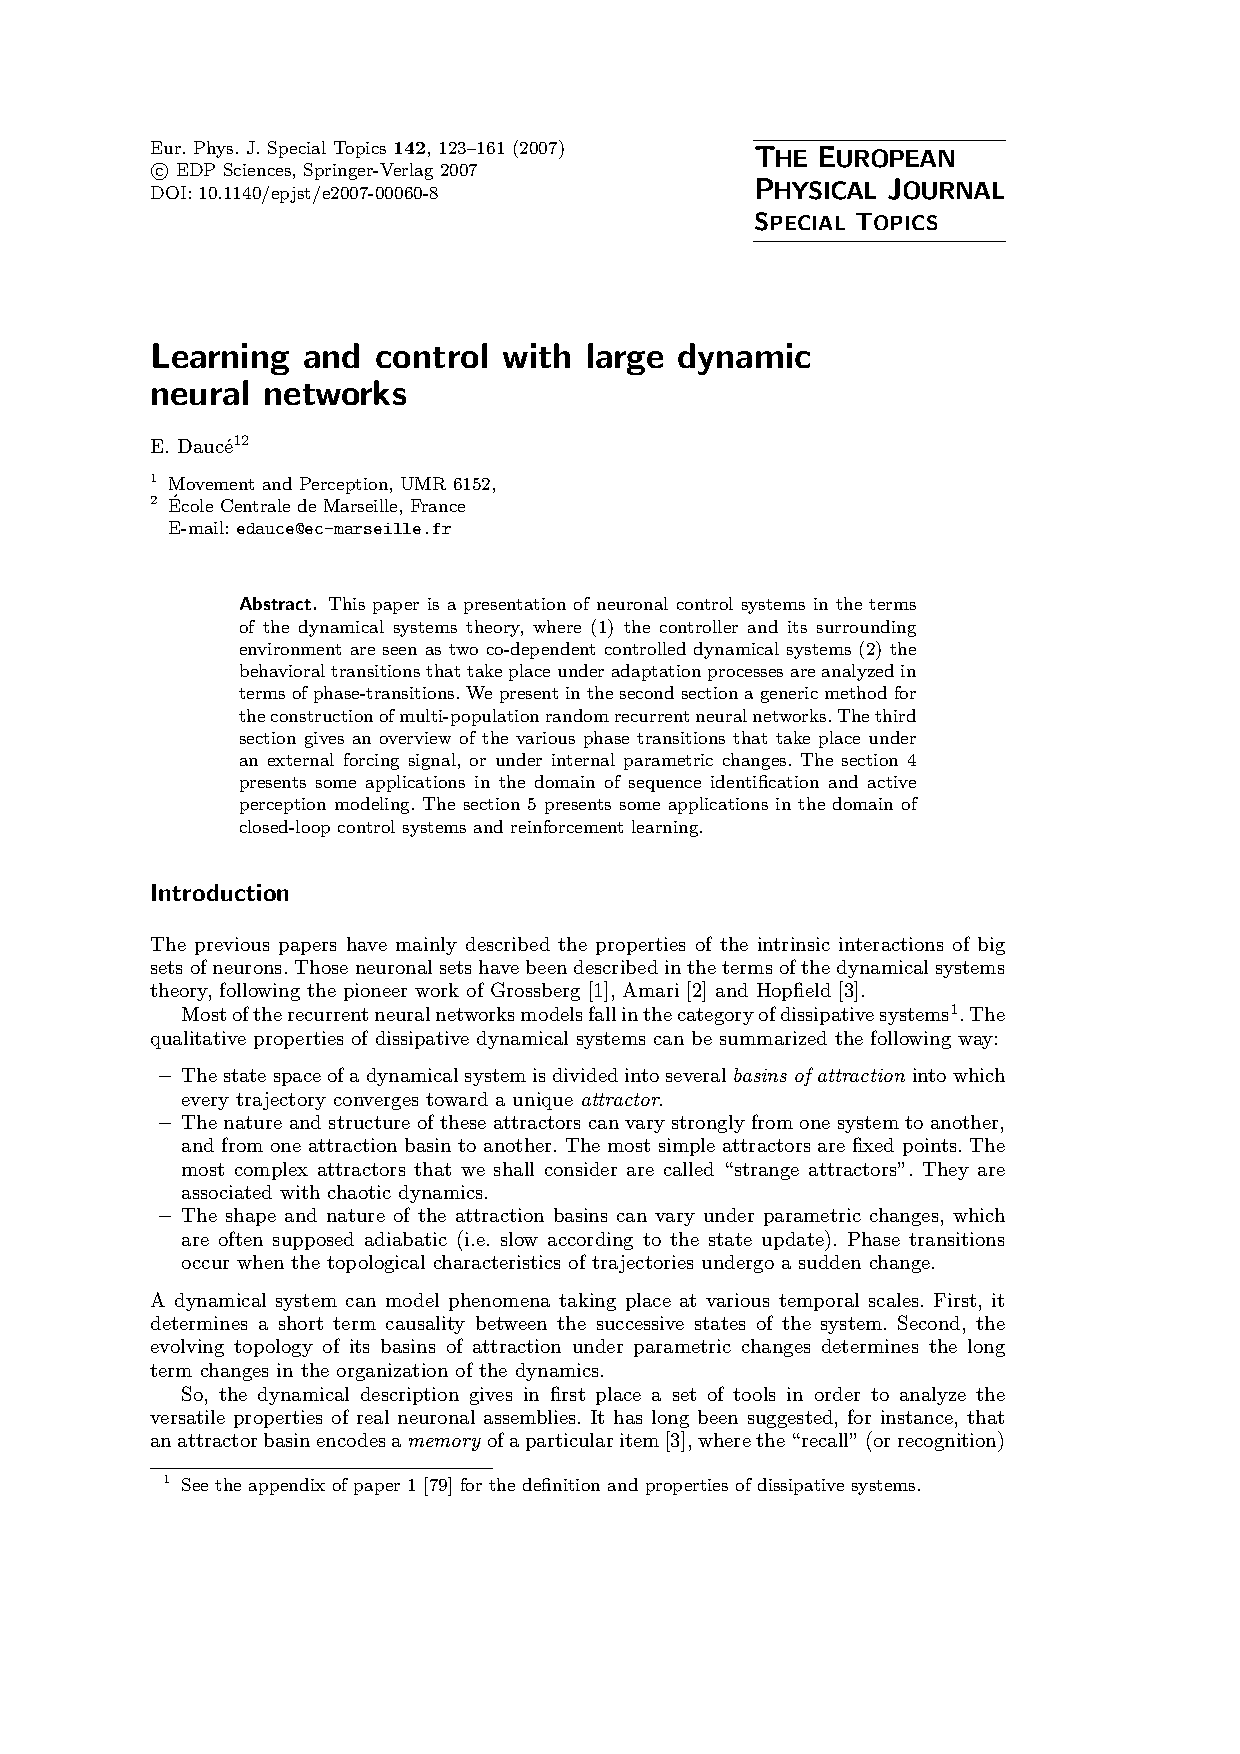
\includepdf[pages=1-10]{pdf/epj-st-2007.pdf}
%\end{minipage}
%}
% Histoires


%%%%%%%%%%%%%%%%%%%%%%%%%%%%%%%%%%%%%%%%%%%%%%%%%%%%%%%%%%%%%%%%%%%%%%%%%%%%%%%%%%%%%%%%%%%%%%%%%%%%%%%%%%%%%%%%%%%
%%%%%%%%%%%%%%%%%%%%%%%%%%%%%%%%%%%%%%%%%%%%%%%%%%%%%%%%%%%%%%%%%%%%%%%%%%%%%%%%%%%%%%%%%%%%%%%%%%%%%%%%%%%%%%%%%%%
%%%%%%%%%%%%%%%%%%%%%%%%%%%%%%%%%%%%%%%%%     4      %%%%%%%%%%%%%%%%%%%%%%%%%%%%%%%%%%%%%%%%%%%%%%%%%%%%%%%%%%%%%%
%%%%%%%%%%%%%%%%%%%%%%%%%%%%%%%%%%%%%%%%%%%%%%%%%%%%%%%%%%%%%%%%%%%%%%%%%%%%%%%%%%%%%%%%%%%%%%%%%%%%%%%%%%%%%%%%%%%
%%%%%%%%%%%%%%%%%%%%%%%%%%%%%%%%%%%%%%%%%%%%%%%%%%%%%%%%%%%%%%%%%%%%%%%%%%%%%%%%%%%%%%%%%%%%%%%%%%%%%%%%%%%%%%%%%%%

\section{Architectures de contrôle pour les neurosciences}

%%%%%%%%%%%%%%%%%%%%%%%%%%%%%%%%%%%%%%%%%%%%%%%%%%%%%%%%%%%%%%%%%%%%%%%%%%%%%%%%%%%%%%%%%%%%%%%%%%%%%%%%%%%%%%%%%%%

%principe général : 
%- comportement based
%- mapping des architectures de contrôle sur le SNC

Si les principes de fonctionnement élémentaires du système nerveux central (neurones, synapses) 
commencent à être bien connus, 
le fonctionnement intégré du système dans son ensemble reste l'objet de nombreuses conjectures.
L'utilisation de modèles mathématiques et de simulations informatiques permet de proposer des hypothèses 
de fonctionnement et/ou 
de valider certaines hypothèses issues de l'observation. 
Les neurosciences computationnelles sont ainsi la branche de l'informatique qui, d'une part, élabore des modèles de calcul 
inspirés par les hypothèses proposées en neurosciences, et, d'autre part, propose des interprétations
de données biologiques à partir de principes et modèles issus des sciences de l'information.
Selon la typologie classique proposée par David Marr \cite{Marr82}, 
un modèle peut appartenir à différents niveaux de généralité, à savoir le niveau computationnel (la 
logique), 
le niveau algorithmique (encodage et opérations réalisées), et
la réalisation matérielle (le substrat).   

Cette distinction en trois niveaux permet principalement de distinguer ce qui relève de la définition du problème~:
définition de la tâche, en fonction des contraintes physiques et de l'appareillage sensoriel et moteur, d'une part, et
d'autre part ce qui relève de la réalisation (algorithmique) de la tâche, c'est à dire principalement le circuit de 
traitement. C'est, en terminologie informatique, la distinction entre
l'équation à résoudre, la brique logicielle qui la résout et le circuit logique qui l'implémente.
Marr postule une relative indépendance entre les différents niveaux de description, en établissant une
claire séparation entre le substrat, le circuit de traitement et l'espace de la tâche.
Cette séparation correspond assez bien au problème des disparités d'échelle 
évoqué plus haut. La contrainte physique du corps, engagé dans différentes tâches, à des échelles
spatiales macroscopiques et des échelles temporelles lentes d'une part.
La containte du circuit microscopique, constitué d'unité neuronales échangeant rapidement des signaux discrets
d'autre part.
Entre les deux, un niveau architectural, constitué de circuits imbriqués intégrant l'activité de
larges portion du cerveau, 
constituant un niveau de description relativement indépendant des deux autres.
Par contraste avec la méthodologie ``bottom-up'' qui consiste à étudier les
conditions d'émergence de fonctions de haut niveau à partir d'un substrat plongé dans un
environnement contraignant, la méthodologie ``top-down'' consiste à étudier les conditions de réalisation
d'une certaine tâche par étapes descendantes, de la contrainte générale du corps engagé dans la tâche
à la réalisation matérielle du circuit qui la résout.

Une approche descendante bien menée consiste souvent à identifier les aspects non-triviaux
d'une tâche. L'étude des temps de réponse, des courbes d'apprentissage et des
taux d'erreur permet d'explorer les caractéristiques limites d'un comportement et de mieux appréhender
les contraintes posées par système qui l'implémente physiquement.
Ce peuvent être des contraintes physiques (limites d'extension, de course, ...) mais
également des limites provenant des caractéristiques physiques du système neuronal sous-jacent.
L'élaboration d'un modèle descriptif prenant en compte plusieurs échelles permet alors d'émettre des hypothèses 
sur les sources (physiques ou logiques) des limitations comportementales observées. 
Nous avons vu dans les parties précédentes des modèles constitués de quelques 
centaines de neurones développant une activité autonome, s'organisant sous la pression d'un signal externe et 
se transformant sous l'effet de la plasticité synaptique.
%La connectivité entre le cortex et les structures sous-corticales (striatum, ganglions de la base, thalamus,
%amygdale, hippocampe, cervelet, ...) met en évidence de nombreuses boucles réentrantes suggérent une 
%prépondérance de l'activité interne sur les entrées sensorielles. Comprendre le rôle de ces boucles
%réentrantes est un des grands enjeux actuels.
La simulation de circuits corticaux et sous-corticaux 
plus fidèles aux observations anatomiques permet de tester la validité de certaines hypothèses en assignant
des fonctions spécifiques aux différentes structures participant au circuit et en étudiant les conditions permettant
au circuit de produire une activité répondant aux contraintes fonctionnelles. 


%On distingue ainsi chez la lamproie trois grandes catégories d'activités motrices, à savoir 

D'un point de vue architectural, il existe de nombreuses preuves d'une organisation parallèle
du système nerveux, avec de nombreux circuits dédiés à des tâches distinctes.  
L'étude d'organismes relativement primitifs permet 
d'identifier les tâches élémentaires, celles qui sont présentes à
tous les niveaux du règne animal et qui structurent l'organisation du système nerveux central.
On distingue ainsi classiquement l'orientation (déplacement les organes des sens vers les stimuli d'intérêt, 
éloignement et évitement des stimuli aversifs), 
la locomotion (déplacement du corps) 
et l'ensemble des comportements consistant à utiliser les ressources de l'environnement (activité alimentaire
par exemple) \cite{brembs03,Grillner2008,Stephenson2011}.
En particulier, un circuit parmi les plus primitifs est celui 
de la sélection de l'action organisé autour des structures sous-corticales (ganglions de la base) 
fonctionnant par désinhibition  
sélective de choix d'actions concurrents, comme mis en évidence par 
\cite{Grillner2008}. 
La dérivation de la commande motrice à travers le cervelet conduit par ailleurs
à des ajustements posturaux associés à un contrôle fin et adaptatif des commandes motrices \cite{Wolpert1998,Zeeuw1998}.
D'autres circuits plus récents, comme ceux de l'hippocampe, 
sont impliqués dans la navigation spatiale, et la mémorisation \cite{McClelland1995},  
exprimant en particulier la situation de l'animal dans un environnement connu mémorisé (son territoire) 
d'un point de vue extérieur, implémentant un mécanisme d'orientation dans un
référentiel extéro-centré \cite{OKe78}. 
Les boucles entre le cortex, le striatum et le cervelet semblent également associées 
chez certains mammifères à la simulation motrice
précédent le déclenchement de l'action \cite{Jeannerod2001}, etc.

A travers deux projets ANR, j'ai pu aborder ces aspects de modélisation selon ces différents niveaux 
autour de l'étude des comportements d'orientation. 
Dans le cadre du projet MAPS déjà présenté, j'ai participé à une étude portant 
sur l'orientation visuelle à partir des données anatomiques et électrophysiologiques du tectum 
et des neurones prémoteurs du tronc cérébral,
en collaboration avec Alain Guillaume, travaillant à l'Institut des Sciences du Mouvement, 
et Anthony Mouraud, qui a effectué un séjour
post-doctoral en 2010 sous notre supervision. 
Dans le cadre du projet ANR NOAT, en collaboration avec Jennifer Coull (LNC, Marseille) et 
Daniele Schön (INCM, Marseille), j'ai également travaillé sur des modèles génératifs du comportement 
d'orientation temporelle,
en collaboration avec Gaurav Malhotra qui a effectué un séjour postdoctoral en 2010-2011 sur cette question.


%%%%%%%%%%%%%%%%%%%%%%%%%%%%%%%%%%%%%%%%%%%%%%%%%%%%%%%%%%%%%%%%%%%%%%%%%%%%%%%%%%%%%%%%%%%%%%%%%%%%%%%%%%%%%%%%%%%
%%%%%%%%%%%%%%%%%%%%%%%%%%%%%%%%%%%%%%%%%     4.1      %%%%%%%%%%%%%%%%%%%%%%%%%%%%%%%%%%%%%%%%%%%%%%%%%%%%%%%%%%%%
%%%%%%%%%%%%%%%%%%%%%%%%%%%%%%%%%%%%%%%%%%%%%%%%%%%%%%%%%%%%%%%%%%%%%%%%%%%%%%%%%%%%%%%%%%%%%%%%%%%%%%%%%%%%%%%%%%%

\subsection{Modèles de l'orientation spatiale}

Un des buts du projet ANR MAPS était de proposer une modélisation du comportement d'orientation visuelle,  à travers
l'étude du système saccadique. Ce système, situé dans le tectum (partie supérieure du tronc cérébral) 
au niveau des couches profondes
du colliculus supérieur, développe une activité topographiqement organisée responsable de la commande
des mouvements rapides des globes oculaires.
%, certains aspects de la commande (déplacement relatif) semblant directement
%liés à la position du foyer d'activité à la surface du colliculus, et d'autres aspects (comme la vitesse de déplacement)
%semblant liés à la fréquence de décharge des neurones.

La saccade oculaire est un mouvement présent chez l'ensemble des vertébrés consistant à orienter 
la partie centrale de la rétine (la fovea) vers un point d'intérêt de l'espace visuel.
Le comportement d'orientation saccadique, par opposition aux comportements locomoteurs
ou alimentaires, est constitué de mouvements brefs (discrets), permettant 
d'explorer la scène visuelle. La saccade oculaire est le prototype des mouvements 
dits ``balistiques'', partant d'une posture initiale et s'achevant sur une posture finale
(par opposition a des mouvements d'ajustement ou de contrôle guidé par 
un feedback comme la poursuite oculaire par exemple).

Etant donnée une cible visuelle présente en périphérie de la rétine, la tâche consiste à positionner 
le corps (tronc, tête et globe oculaire) de telle sorte que cette cible soit placée au centre de la rétine.
Le mouvement consiste donc, étant donnée la posture corps-tête-oeil initiale, à produire
un déplacement corps-tête-oeil conduisant à la posture cible finale. La séquence qui, à partir des données
sensorielles et proprioceptives, génère une activité phasique (une bouffée d'activité) des motoneurones 
conduisant au déplacement désiré est appelée la transformation visuo-motrice (dite
transformation ``spatio-temporelle'' \cite{MOSCHO98}). 
Elle implique la traduction d'une activité exprimant des coordonnées spatiales   
vers une activité temporellement bornée exprimant une vélocité motrice transitoire.
Une version simplifiée de la tâche est la saccade à tête fixe consistant orienter le globe
oculaire seul.

Même si on se limite aux saccades à tête fixe, le circuit de la commande saccadique demeure assez complexe
et non totalement élucidé. Si l'on exclut les étapes de traitement visuel conduisant à l'identification
d'un point d'intérêt en périphérie de la rétine, la structure au carrefour de la transformation 
visuo-motrice est
une carte rétinotopique située sur la partie supérieure du tectum,
appelée le colliculus supérieur. 
Le déclenchement de la saccade implique 
de nombreuses catégories de neurones du tronc cérébral, incluant des inhibiteurs toniques,
des neurones prémoteurs excitateurs et inhibiteurs variés appartenant à la formation réticulée, 
une dérivation via le cervelet et enfin des motoneurones oculaires. 

Le colliculus est une carte topographique bilatérale (champ visuel droit, champ visuel gauche) 
dont la stimulation électrique permet de déclencher des saccades.
L'amplitude des saccades dépend de la position de la stimulation sur la carte, et non de la fréquence 
ou de l'intensité de la stimulation. 
La commande motrice étant ballistique (sans feedback visuel ou proprioceptif),
les premiers travaux de modélisation \cite{Rob75} suggèrent l'existence d'un intégrateur
dans le circuit de la commande déterminant la durée de la saccade en fonction de la  
distance déjà parcourue (intégration de la commande de vitesse au cours du temps).
%La commande est alors proportionnelle à l'erreur motrice (la distance restant à parcourir).
Pour tenir compte de certaines observations (en particulier la résistance à
des variations de fréquences conduisant à des saccades plus lentes mais toujours précises),
l'hypothèse d'un chemin double contrôlant à la fois la vitesse et la durée 
de la saccade a été émis par \cite{Groh2001}.

Le travail réalisé en collaboration avec Alain Guillaume et Anthony Mouraud a consisté à étudier 
et implémenter sur un simulateur de réseaux de neurones réaliste cette hypothèse de chemin double
vers les neurones prémoteurs. 
Le logiciel utilisé est le simulateur de neurones impulsionnels ``DAMNED'' 
développé par Anthony Mouraud et Didier Puzenat \cite{Mouraud2009}. 
Notre modèle étudie la transformation sensori-motrices à l'aide d'une architecture réaliste
impliquant plusieurs milliers de neurones. La carte colliculaire est organisée de manière topographique
selon un principe de champ neuronal (connexions excitatrices à courte distance, connexions
inhibitrices à longue distance). Les projections directes des neurones colliculaires vers les neurones pré-moteurs
obéissent à un gradient exponentiel, l'amplitude de la saccade augmentant non linéairement
avec l'excentricité. 

Notre modèle repose sur l'hypothèse d'un contrôle effectué selon trois modalités:
contrôle du déclenchement, contrôle de la vélocité et contrôle de la durée.
Si la vélocité repose bien sur les projection directe du coliculus vers les neurones pré-moteurs,
nous faison l'hypothèse que le contrôle du déclenchement et le contrôle de la durée reposent 
sur une structure de la formation réticulée appelée cMRF (centro-medial reticular formation)
dont le rôle dans le contrôle de la saccade est connu \cite{Waitzman1996}.  

Un premier modèle, présenté à l'édition 2011 de la conférence CNS \cite{Dauce2011}, attribue un rôle double
aux cellules du CMRF. Les cellules contralatérales règlent le déclenchement de la saccade tandis que les cellules 
ipsilatérales participent à sa terminaison via une intégration sous-liminaire du signal émis par les 
neurones pré-moteurs. Ce modèle utilise des neurones dont la constante de membrane lente 
permet de faire l'économie d'un mécanisme d'intégration plus élaboré. La brève bouffée 
émise par les neurones ipsilatéraux lorsque le potentiel atteint le seuil interrompt 
simultanément l'activité des neurones prémoteurs et celle du colliculus, mettant fin à 
la saccade.

Ce premier modèle, de fonctionnement relativement simple, ne prend pas en compte certaine observations qui 
reportent une prise en compte par le système saccadique de l'activité effective des neurones pré-moteurs \cite{Barton2003}.
Un second modèle, incluant un lien de feedback des neurone prémoteurs vers les neurones du cMRF
a été implémenté. Ce modèle, qui permettait de prendre en compte l'interruption temporaire de l'activité
des neurones prémoteurs présentait néanmoins des tracés de saccades moins précis, et n'a pas fait l'objet de publication.

Cette étude, en implémentant de façon très détaillée les populations de neurones en jeu, a permis de 
souligner l'importance sans doute sous-évaluée des neurones du cMRF dans le contrôle de la saccade. Néanmoins, 
le nombre et la complexité des paramétres en jeu (types de neurones, constantes d'intégration, types et amplitude
des projection, nombre de populations, existence ou absence de certains faisceaux d'axones, ...) 
rend difficiles à distinguer les facteurs contribuant à la réussite ou à l'échec du modèle
(défaut de conception, défaut de réalisme, défaut de paramétrage, défaut d'implémentation).
La prise en compte de conditions plus générales (saccades libres, saccades adaptatives, cibles en 
mouvement) nécessiterait la mise en oeuvre de modèles de populations plus simples, basés sur des masses neuronales plutôt
que des neurones détaillés. Certains des principes 
computationnels évoqués plus haut, comme l'idée d'un contrôle basé sur des
points fixe de l'espace de postures, pourraient être développés dans ce cadre. 
Cet aspect sera présenté plus précisément dans la partie projet de ce mémoire. 

{\color{Violet}
{\bf 2010}

- A. Mouraud : mecanisme integrateur. Dual drive. 
}

%%%%%%%%%%%%%%%%%%%%%%%%%%%%%%%%%%%%%%%%%%%%%%%%%%%%%%%%%%%%%%%%%%%%%%%%%%%%%%%%%%%%%%%%%%%%%%%%%%%%%%%%%%%%%%%%%%%
%%%%%%%%%%%%%%%%%%%%%%%%%%%%%%%%%%%%%%%%%     4.2      %%%%%%%%%%%%%%%%%%%%%%%%%%%%%%%%%%%%%%%%%%%%%%%%%%%%%%%%%%%%
%%%%%%%%%%%%%%%%%%%%%%%%%%%%%%%%%%%%%%%%%%%%%%%%%%%%%%%%%%%%%%%%%%%%%%%%%%%%%%%%%%%%%%%%%%%%%%%%%%%%%%%%%%%%%%%%%%%

\subsection{Modèles de l'orientation temporelle}

{\bf 2010}

- Gaurav : attention temporelle. Modele EM. 


{\bf 2011}

- scalar property

$\Rightarrow$ prior $\simeq$ ``\% up to now'' (subjective time)


%%%%%%%%%%%%%%%%%%%%%%%%%%%%%%%%%%%%%%%%%%%%%%%%%%%%%%%%%%%%%%%%%%%%%%%%%%%%%%%%%%%%%%%%%%%%%%%%%%%%%%%%%%%%%%%%%%%
%%%%%%%%%%%%%%%%%%%%%%%%%%%%%%%%%%%%%%%%%     4.3      %%%%%%%%%%%%%%%%%%%%%%%%%%%%%%%%%%%%%%%%%%%%%%%%%%%%%%%%%%%%
%%%%%%%%%%%%%%%%%%%%%%%%%%%%%%%%%%%%%%%%%%%%%%%%%%%%%%%%%%%%%%%%%%%%%%%%%%%%%%%%%%%%%%%%%%%%%%%%%%%%%%%%%%%%%%%%%%%




%%%%%%%%%%%%%%%%%%%%%%%%%%%%%%%%%%%%%%%%%%%%%%%%%%%%%%%%%%%%%%%%%%%%%%%%%%%%%%%%%%%%%%%%%%%%%%%%%%%%%%%%%%%%%%%%%%%
%%%%%%%%%%%%%%%%%%%%%%%%%%%%%%%%%%%%%%%%%%%%%%%%%%%%%%%%%%%%%%%%%%%%%%%%%%%%%%%%%%%%%%%%%%%%%%%%%%%%%%%%%%%%%%%%%%%
%%%%%%%%%%%%%%%%%%%%%%%%%%%%%%%%%%%%%%%%%%%%%%%%%%%%%%%%%%%%%%%%%%%%%%%%%%%%%%%%%%%%%%%%%%%%%%%%%%%%%%%%%%%%%%%%%%%
%%%%%%%%%%%%%%%%%%%%%%%%%%%%%%%%%%%%%%%%%%%%%%%%%%%%%%%%%%%%%%%%%%%%%%%%%%%%%%%%%%%%%%%%%%%%%%%%%%%%%%%%%%%%%%%%%%%
%%%%%%%%%%%%%%%%%%%%%%%%%%%%%%%%%%%%%%%%%%%%%%%%%%%%%%%%%%%%%%%%%%%%%%%%%%%%%%%%%%%%%%%%%%%%%%%%%%%%%%%%%%%%%%%%%%%
%%%%%%%%%%%%%%%%%%%%%%%%%%%%%%%%%%%%%%%%%%%%%%%%%%%%%%%%%%%%%%%%%%%%%%%%%%%%%%%%%%%%%%%%%%%%%%%%%%%%%%%%%%%%%%%%%%%
\chapter{Projet scientifique}
%%%%%%%%%%%%%%%%%%%%%%%%%%%%%%%%%%%%%%%%%%%%%%%%%%%%%%%%%%%%%%%%%%%%%%%%%%%%%%%%%%%%%%%%%%%%%%%%%%%%%%%%%%%%%%%%%%%
%%%%%%%%%%%%%%%%%%%%%%%%%%%%%%%%%%%%%%%%%%%%%%%%%%%%%%%%%%%%%%%%%%%%%%%%%%%%%%%%%%%%%%%%%%%%%%%%%%%%%%%%%%%%%%%%%%%
%%%%%%%%%%%%%%%%%%%%%%%%%%%%%%%%%%%%%%%%%%%%%%%%%%%%%%%%%%%%%%%%%%%%%%%%%%%%%%%%%%%%%%%%%%%%%%%%%%%%%%%%%%%%%%%%%%%
%%%%%%%%%%%%%%%%%%%%%%%%%%%%%%%%%%%%%%%%%%%%%%%%%%%%%%%%%%%%%%%%%%%%%%%%%%%%%%%%%%%%%%%%%%%%%%%%%%%%%%%%%%%%%%%%%%%
%%%%%%%%%%%%%%%%%%%%%%%%%%%%%%%%%%%%%%%%%%%%%%%%%%%%%%%%%%%%%%%%%%%%%%%%%%%%%%%%%%%%%%%%%%%%%%%%%%%%%%%%%%%%%%%%%%%
%%%%%%%%%%%%%%%%%%%%%%%%%%%%%%%%%%%%%%%%%%%%%%%%%%%%%%%%%%%%%%%%%%%%%%%%%%%%%%%%%%%%%%%%%%%%%%%%%%%%%%%%%%%%%%%%%%%

D'un point de vue général, les opérations du système nerveux se caractérisent par un compromis entre des opérations 
essentiellement produites par l'activité interne, et des opérations guidées par les stimulations sensorielles. 
L'analyse de la communication nerveuse implique la prise en compte du cadre macroscopique des interactions entre 
le système nervveux, l'appareil sensori-moteur et son milieu.
La correspondance entre l'activité macroscopique et l'activité nerveuse reste à ce jour non élucidé.

L'analyse que nous avons développée à partir de l'étude des réseaux de neurones aléatoires suggère un mode de fonctionnement
intermédiaire entre le pattern matching et les systèmes dynamiques. Plus précisément, nous avonc utilisé l'exemple (ou l'analogie)
d'un système dynamique distribué contraint par un signal extérieur. 

Les différentes études présentées permettentde soulever de nombreuses questions sur les principes computationnels 
à l'oeuvre au sein de l'activité nerveuse,
listées ci-desous.

\paragraph{Nature du feedback} 
Un des schémas proposés ici pour la communication nerveuse 
est celui du feedback positif, autrement
dit la résonance entre l'activité macroscopique et l'activité nerveuse, caractérisée par la présence d'un attracteur comportemental 
(posture ou patron d'interaction dynamique). L'hypothèse est que le substrat nerveux est un réservoir de patrons sensori-moteurs, 
et l'apparition de précurseurs sensoriels ou moteurs au sein de l'activité nerveuse suscite la convergence de la dynamique vers l'attracteur correspondant, 
favorisant une activité macroscopique (un attracteur comportemental) qui lui-même favorise l'attracteur neuronal par boucle de rétroaction positive.
Des mécanismes internes de fatigue et/ou l'irruption de composants sensoriels ou moteurs dissonants favorise la recomposition de l'activité nerveuse
et la convergence vers un nouvel attracteur.

Ce schéma computationnel (fonctionnement par ``sauts'' d'un attracteur à un autre, alternance entre destabilisation et 
stabilité) n'est pas exclusif du schéma traditionnel du guidage de l'activité motrice par l'activité sensorielle (schéma
à feedback négatif).  Autrement dit, rien ne permet d'exclure que l'activité nerveuse, 
caractérisée microscopiquement par des patrons de connexion 
excitateurs et inhibiteurs, puisse susciter à la fois des schémas comportementaux basés 
sur le feedback positif (persévération, résistance au changement
et changements brusques) et le feedback négatif (réponse graduelle à l'erreur perceptive, poursuite lente, ...).

Question ouverte : quelles sont les contributions respectives de ces deux approches à l'activité neuronale? Quelles prédictions?

{\color{Violet}}
Les schémas de guidage par correction d'erreur sont très présents au niveau des structures sensori-motrices profondes
(comme le contrôle vestibulaire).

l'approche par feedback négatif repose principalement sur le calcul d'une erreur de prédiction. 
On suppose donc l'existence d'un modèle interne qui 
anticipe la conséquence sensorielle de l'action [WOLPERT], et corrige éventuellement
le modèle si cette 

Une des prédictions, pour distinguer l'un de l'autre, serait d'identifier une activité liée à l'erreur perceptive. 
vs une activité liée au matching perceptif (correspondance)

}

\paragraph{Espace métrique et espace logique}

Les déplacements produits par le corps en mouvement sont tous quantifiables par la position (et les variations de position) 
des éléments mobiles qui le composent.
Les sources de l'activité induite sur les organes sensoriels sont également localisables dans un espace métrique
tridimensionnel constituant l'environnement immédiat du sujet.
Il est pourtant relativement difficile d'identifier au sein du cerveau des activités (ou des variations d'activité) en lien 
avec cet espace métrique. 
Par exemple, il est possible d'établir des corrélations entre l'activité mesurée sur les neurones du cortex moteurs et le
mouvement effectif, mais corrélations ne permettent pas (ou permettent difficilement) de reconstruire une 
trajectoire métrique précise.

Le caractère extrêmement distribué de l'activité nerveuse suggère la distribution de ces quantités sur de nombreux neurones.
En particulier, il apparaît probable qu'une même quantité n'active pas les même neurones selon sa position
dans un certain intervalle de valeurs. 
Cette distribution de l'activité rend néanmoins difficile la réalisation d'opérations simples comme l'addition ou la différence
de deux quantités, comme celà est pourtant nécessaire lorsque les déplacements doivent prendre en compte des sources sensorielles 
multiples (proprioception de la position de la tête et excentricité d'une cible sur la rétine par exemple).
Si l'espace métrique environnant est décomposé en composants élémentaires (intervalles ou ``pixels'' d'environnement), activant
ou désactivant différentes populations de neurones, alors les opérations élémentaires de translation, rotation, co-extension, 
etc. doivent être apprises ``par coeur'' et ne peuvent résulter de la combinaison d'activités unitaires.

Si le contrôle de l'appareil moteur, ou plus généralement l'activité d'orientation, repose sur ces principes, 
l'apprentissage de la combinaison des facteurs reste un problème ouvert. En effet, s'il est facile d'exprimer une erreur 
(une distance) dans un espace métrique, il est plus difficile d'exprimer cette même distance, et donc la correction
nécessaire dans un espace ``qualitatif'' distribué. 

IDEE : apprentissage des corrections motrices : pour un certain canal (activité distribuée) mapping entre proprioception
et perçue et désirée. activité du cervelet?


%La traduction de l'espace qualitatif neuronal vers l'espace quantitatif 
%métrique passe des essais/erreurs, récompensé lorsque la commande atteint le but par hasard, et donc un apprentissage lent. 
%Le caractère rapide des corrections opérées par le système sensori-moteur suggère donc que la  


la multitude des combinaisons motrices et sensorielles rend difficile (impossible) l'attribution
d'une seule quantité aux différents neurones : si une quantité peut être exprimée par de nombreux neurones, un même neurone
doit lui-même être l'expression de nombreuses quantités, changeant de rôle selon le contexte.  

La question de l'expressivité des substrats nous permet de soulever la question du caractère métrique ou non métrique 
(quantitatif ou qualitatif) des patrons d'activité produits par l'activité nerveuse.

Le contrôle moteur par correction de l'erreur perceptive repose sur le traitement de signaux quantitatifs (la
force de la commande de correction étant proportionnelle à l'erreur perçue): temps et espace continus.
A l'inverse, le calcul automatique repose sur des opérations séquentielles et discrètes.

Existe-t-il au sein de l'activité du substrat une quantité traduisant la distance entre deux configurations d'activité?

D'un côté, l'information métrique peut être extraite de l'activité de neurones du cortex moteur (reconstuction des trajectoires
à partir de l'activité de différents neurones) [GEORGOPOULOS]. Cette information est néanmoins peu fiable...

@article{wessberg2000real,
  title={Real-time prediction of hand trajectory by ensembles of cortical neurons in primates},
  author={Wessberg, Johan and Stambaugh, Christopher R and Kralik, Jerald D and Beck, Pamela D and Laubach, Mark and Chapin, John K and Kim, Jung and Biggs, S James and Srinivasan, Mandayam A and Nicolelis, Miguel AL},
  journal={Nature},
  volume={408},
  number={6810},
  pages={361--365},
  year={2000},
  publisher={Nature Publishing Group}
}


Approche pattern matching : une succession de correspondances


Une des différences principales concerne le caractère non métrique de cette approche, basée sur la correspondance de forme (pattern matching),
et non sur la différence de forme (erreur entre prédiction et observation).

une activité basée sur la 

\paragraph{Référentiels}

Espace métrique interne. 
Les senseurs sont fortement non-linéaires. 

\paragraph{Réservoir}
L'approche par feedback positif repose sur la prise en compte de la dynamique intrinsèque. Ce sont les caractéristiques
spontanées de cette dynamique qui conditionnent la nature des opérations réalisées, et le type d'interactions possibles entre
le substrat nerveux et son environnement.


\paragraph{Entraînement}
Nous avons cherché à illustrer le caractère parallèle et complémentaire de l'activité nerveuse et de l'activité macroscopique.
Ces deux activités sont largement séparées à la fois par l'échelle spatiale et l'échelle temporelle. 
Seuls l'entrainement de populations nerveuses (interactions longue-distance, synchronisation, résonance) permettent d'expliquer 
l'existence de moments au cours desquels les deux échelles de description se rejoignent pour former un seul et même
système.


L'approche par feedback positif suggère une activité corrélée avec les déplacements moteurs. L'approche par feedback 

Apprentissage par coeur vs. modèle interne

Prédiction d'une activité contingente aux grandeurs physiques (et non à l'erreur perceptive).



Rôle du bruit. Bruit créateur. Formation de patrons d'interaction.


Le caractère distribué des (représentation d'une grandeur physique par l'activité d'une population)

en montrant que certains phénomènes comme la criticalité, 
la résonance, la multistabilité 





Contrairement à l'approche 


et des contraintes


différentes extensivités

La décision 


les théories de la simulatio interne \cite{Jeannerod2001}, ou de l'espace de travail ... \cite{}, stipulent   


\section{Questions ouvertes}


\section{Projets en cours}



\section{Projets à long terme}

Projet :

- MODELE SOUS-CORTICAL POUR TVB

- DIFFERENTS PAPIERS A TERMINER : CRITICALITE, BRUIT TEXTURE ET APPRENTISSAGE, SYNCHRO INDUITE A TRAVERS LES MODELES, ...

- VIBRATIONS

- FRISTON - APPRENTISSAGE - REDUCTION D'INCERTITUDE (DIFFERENT DE REWARD-BASED) - SUBSTRAT -BABBLING - SMC

- SYNCHRO BODY/ENV. - BCI - INVERSE MODELLING

- BINDING + SPATIAL CODING - FIELD COMPUTATION - ATTRACTOR-BASED MOTOR CONTROLE

- ACTIVITE INTRINSEQUE ET ``FREE WILL''

- CHANGEMENT DE REFERENTIEL

{\bf 1999}

- Philo 1 : non-extensivité des sensations - analogie “zone aveugle”

{\bf 2000-2001}

- travail de biblio sur l’hippocampe. 

{\bf 2003-2004}

- Philo 2: pensée à l’échelle temporelle de nos actes

{\bf 2009}

- travail sur les structures sous-corticales : striatum/tectum/cervelet 

{\bf 2010}

- Premier modele (nu,theta)

En particulier : la notion d'expressivité du substrat est prometteuse. 

- Variables de contrôle. Equilibre dynamique. Homeostasie. Emploi et Couplage sans emploi. Répertoire (dictionnaire?) d'emplois. 

- Neurone hédoniste.
IDEE : DU POINT DE VUE DU NEURONE HEDONISTE, LES SPIKES EMIS DOIVENT AVOIR POUR CONSEQUENCE DE MIEUX SOUMETTRE LE NEURONE A DE NOUVELLES STIMULATIONS - PRIOR SUR L’EXPOSITION AUX STIMULATIONS FUTURES.




Perspectives :
\begin{itemize}
\item Substrat apprenant universel
\item Field computation. Patron (fenêtre) d’interaction anisotropique. La reponse n’est pas un vecteur ou un scalaire mais une distribution.
\item Regles de plasticité, information mutuelle et binding. Synchronie des systemes en interaction. Le binding au niveau des schémas d’interaction en miroir. Co-evolution. Mutual information (avec mutual emission et reception). Accrochage de phase. Emergence et non-sens. Independance : est “bindé” ce qui évolue ensemble (non indépendamment). Est “non bindé” ce qui évolue indépendamment. Lié aux DDL? 
$\Rightarrow$ Le substrat est le support de plusieurs processus indépendants. Par analogie au neural field, on peut avoir plusieurs “bulles” sur la carte.
\item idée de perméabilité / imperméabilité des echelles BOTTOM $\rightarrow$ UP. Les etats et les processus des echelles inferieures ne sont pas impactées par les phenomenes d’ordre superieur autrement que par les signaux et les tâches traitées à leur échelle. Exemple : une couche motrice est principalement en train de stabiliser des couplages, pas d’instituer (proclamer/décréter) un nouvel “emploi”. (pas de “downward causation”)
\end{itemize}

\chapter{Conclusion}

Les fondateurs des sciences cognitives ont placé très tôt la question de l'apprentissage  au coeur de leur problématique 
(qu'est-ce qu'une machine intelligente - cf. Turing)

Deux approches/réponses se dessinent dès l'origine :  
\begin{itemize}
 \item traitement symbolique
 \item traitement analogique
\end{itemize}
L'enjeu principal est celui d'un côté du traitement analogique et de l'autre le traitement symbolique. Du point de vue des sciences cognitives naissantes, c'est le traitement
symbolique qui gagne dans un premier temps.

Dans ces deux formalismes, la question de l'apprentissage a eu tendance à progressivement se marginaliser au profit (1) du traitement logique des symboles et de modèles
 descriptifs du langage (grammaires génératives) et (2) l'ingéniérie et la conception de systèmes d'asservissement de plus en plus complexes et/ou psychologie et constructivisme (Palo Alto)

A l'inverse, la question de l'apprentissage est restée présente dans le domaine des sciences de l'information et l'informatique naissante. 
La question de l'apprentissage  devient la question de construire des programmes (des automates) capables de se modifier, de s'amender pour mieux répondre aux sollicitations
de l'environnement. Cette question étant posée (comment modifier le programme sans intervention humaine), le formalisme des réseaux de neurones et du calcul distribué 
s'est révélé le plus apte à traiter la question --> le perceptron. 

\bibliographystyle{apalike}%{apacite}
\bibliography{biblio}


\end{document}
